\section{Результаты}

\subsection{Гистограмма и график плотности распределения}

\begin{figure}[H]
	\begin{tabular}{ccc}
		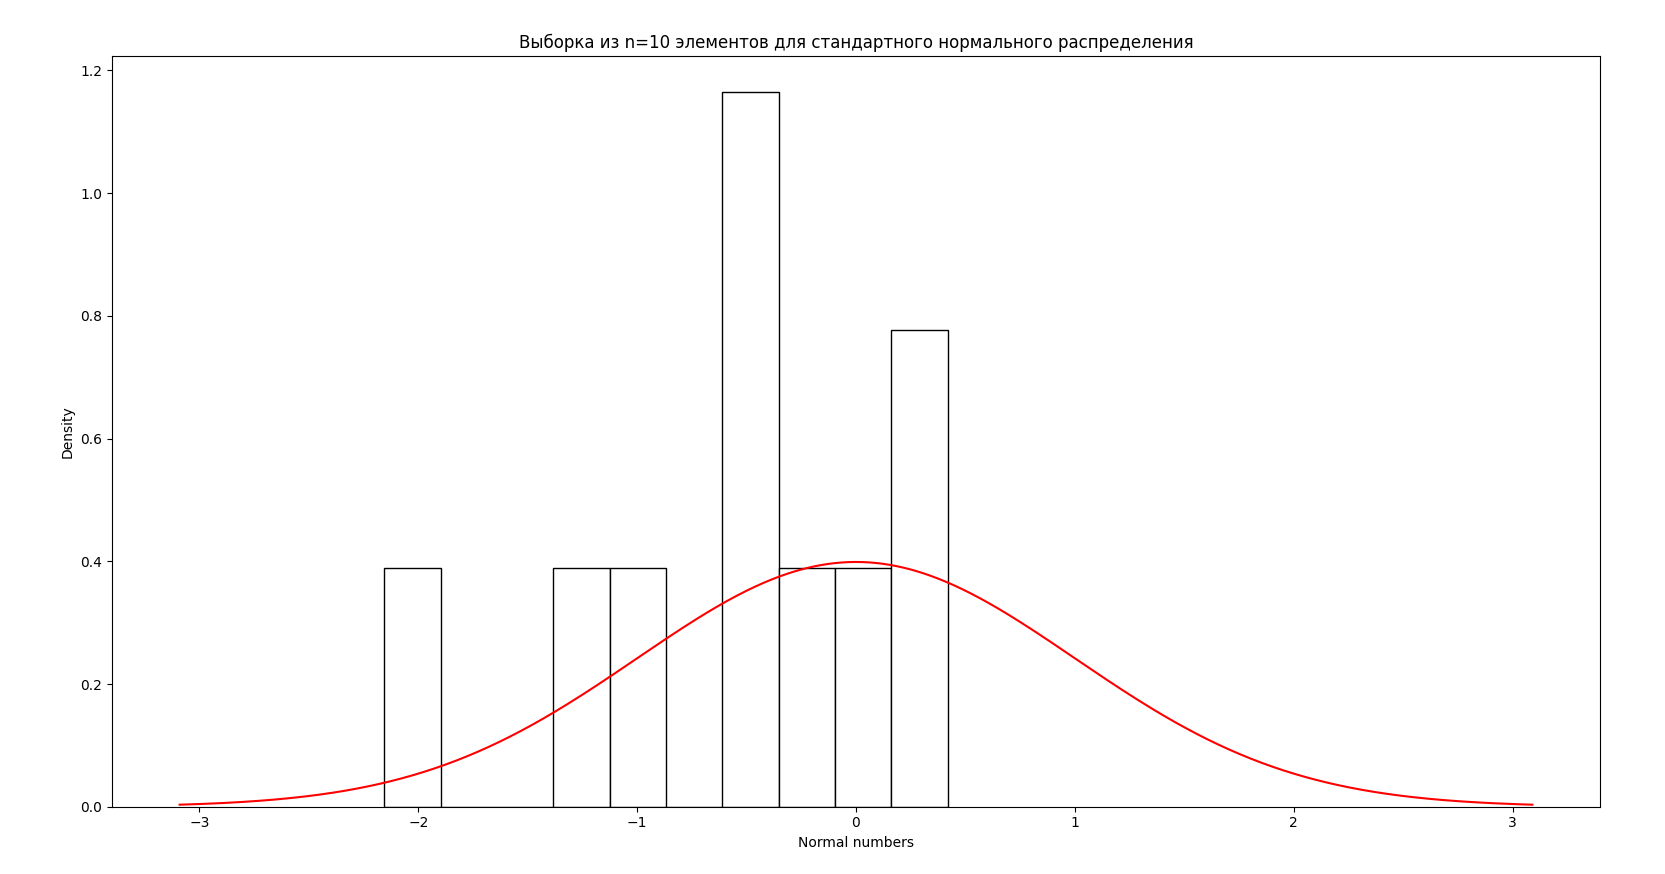
\includegraphics[scale=0.12]{resources/1_gauss_10.png}
		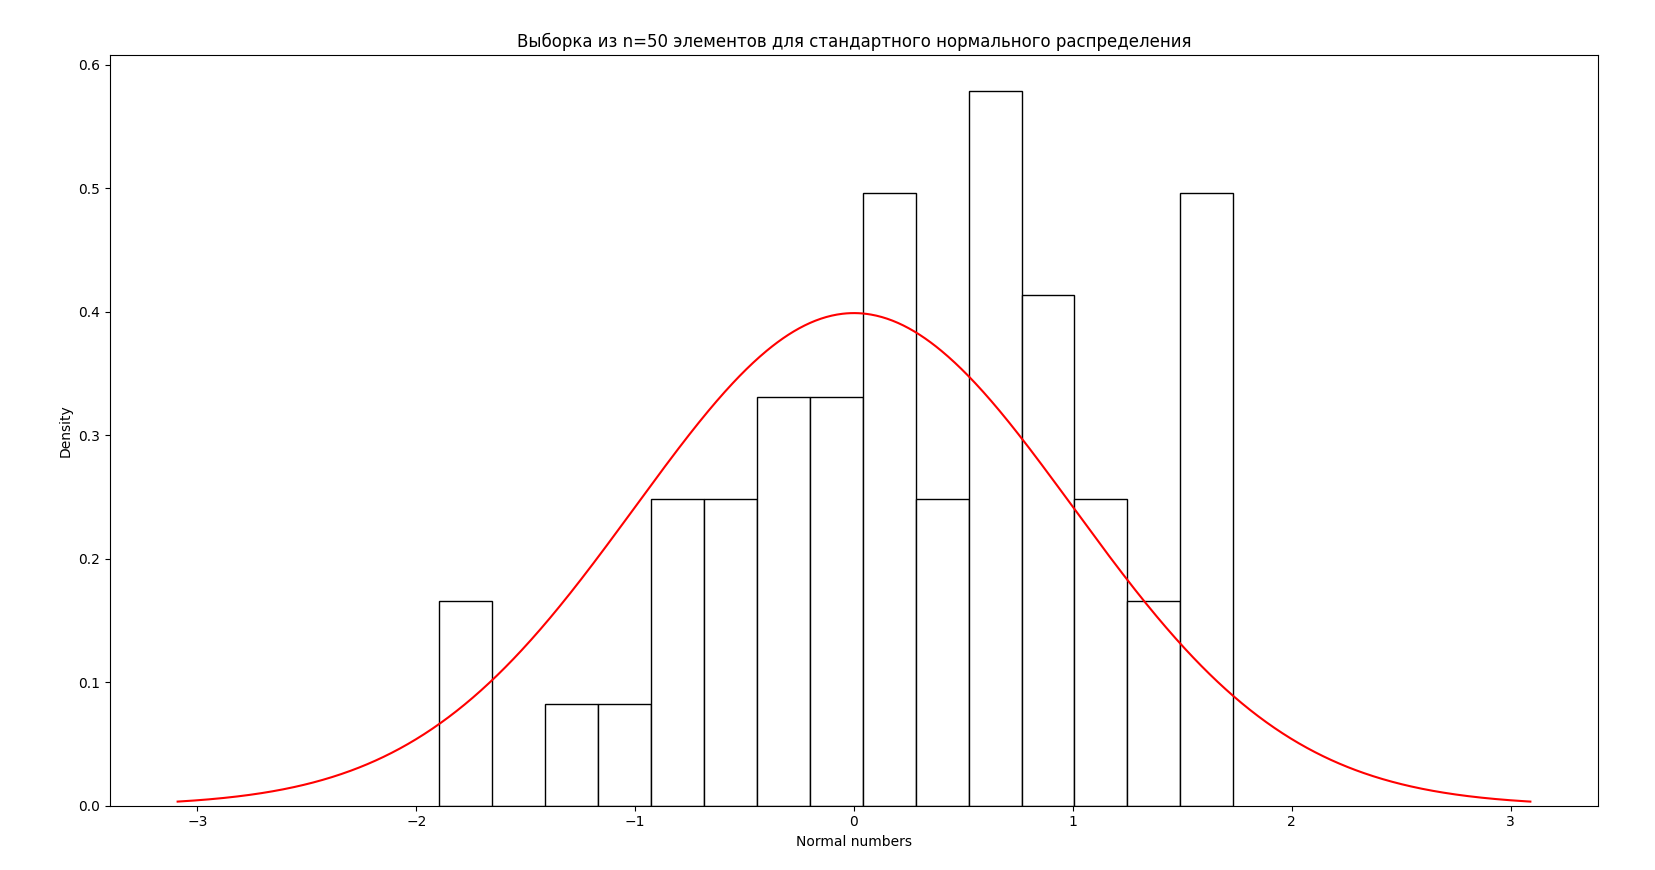
\includegraphics[scale=0.12]{resources/1_gauss_50.png}
		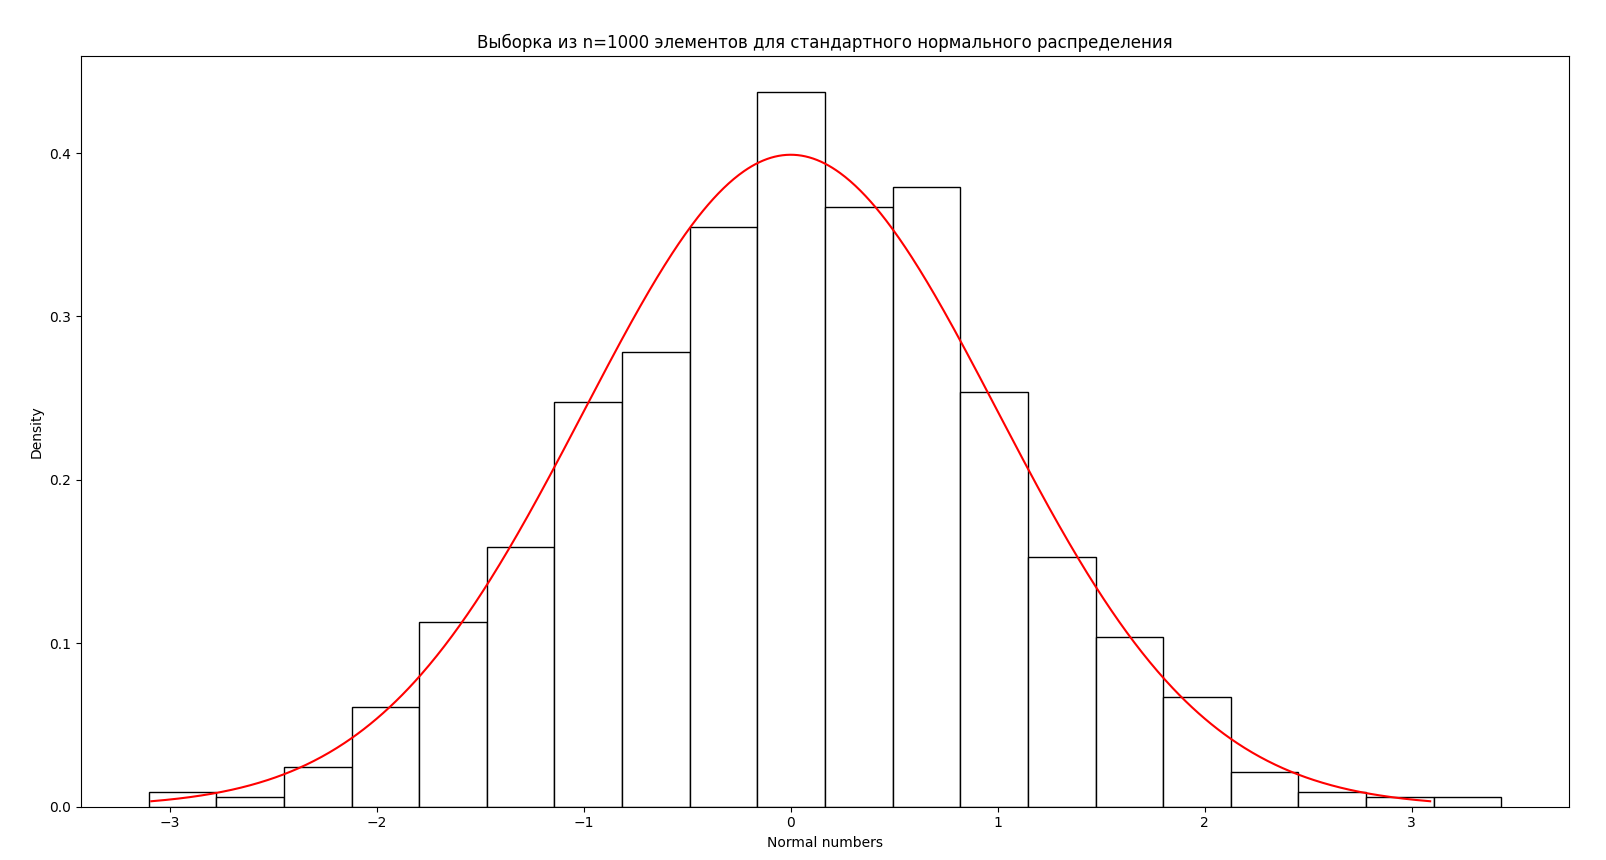
\includegraphics[scale=0.12]{resources/1_gauss_1000.png}
	\end{tabular}
	\caption{Нормальное распределение}
\end{figure}

\begin{figure}[H]
	\begin{tabular}{ccc}
		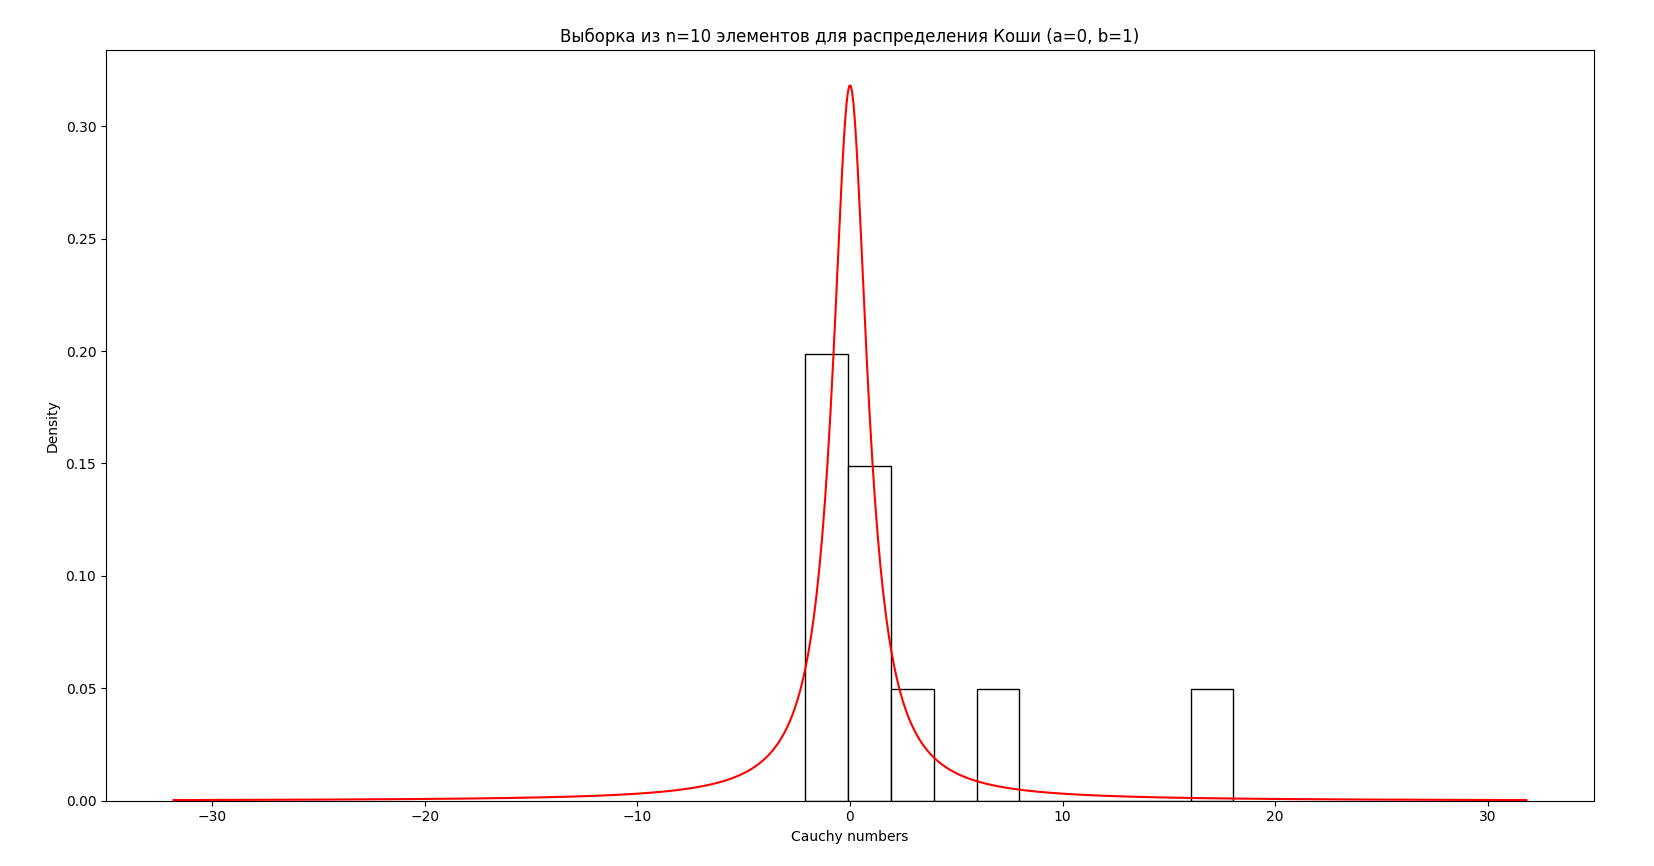
\includegraphics[scale=0.12]{resources/1_cauchy_10.png}
		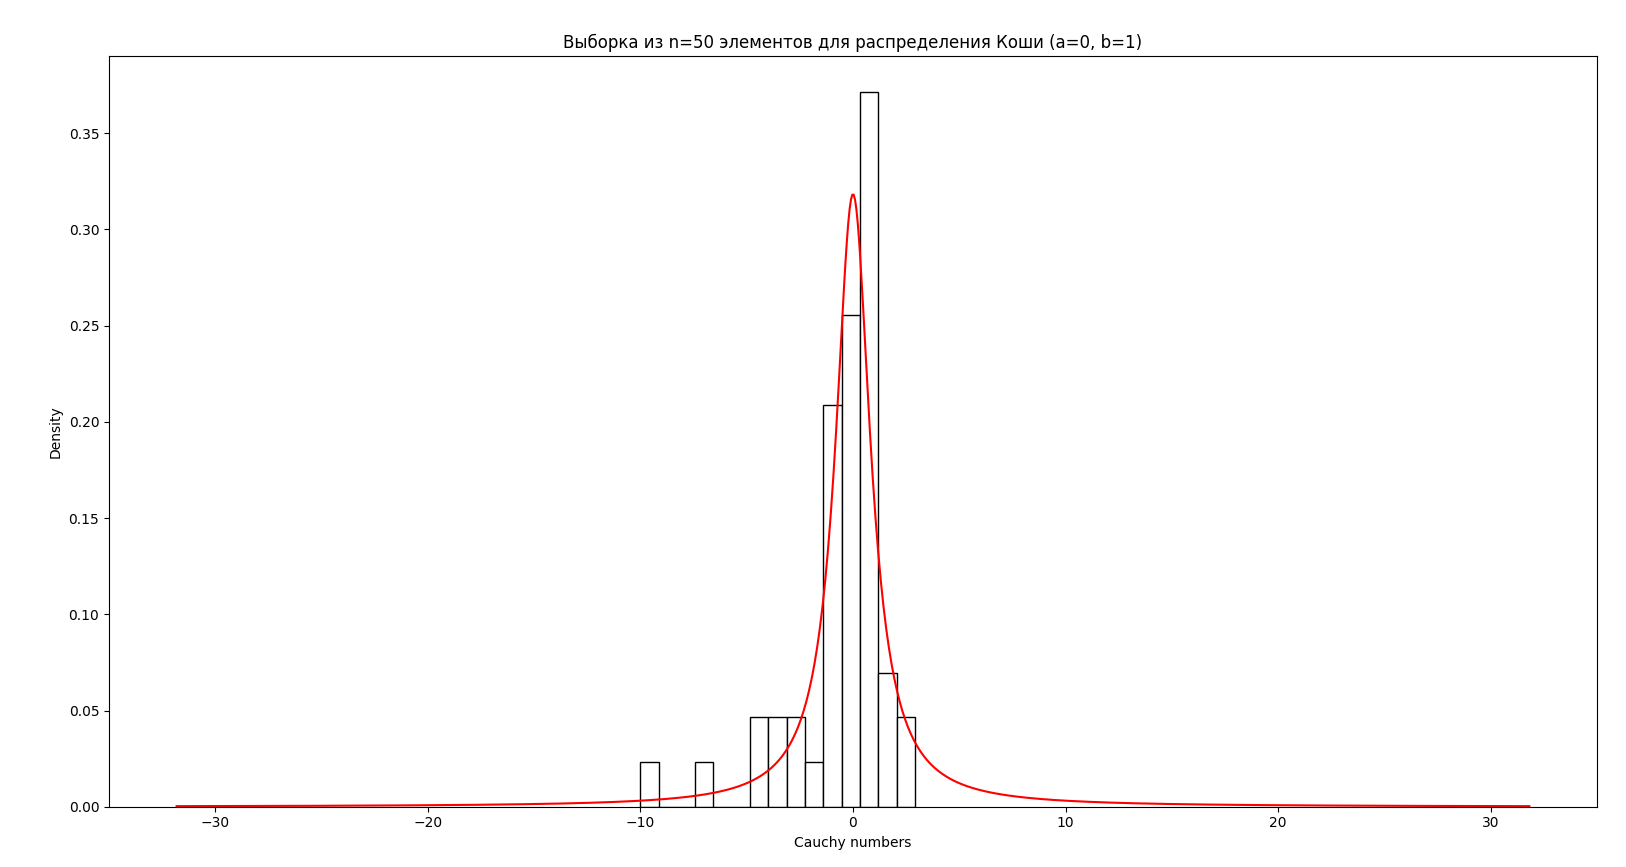
\includegraphics[scale=0.12]{resources/1_cauchy_50.png}
		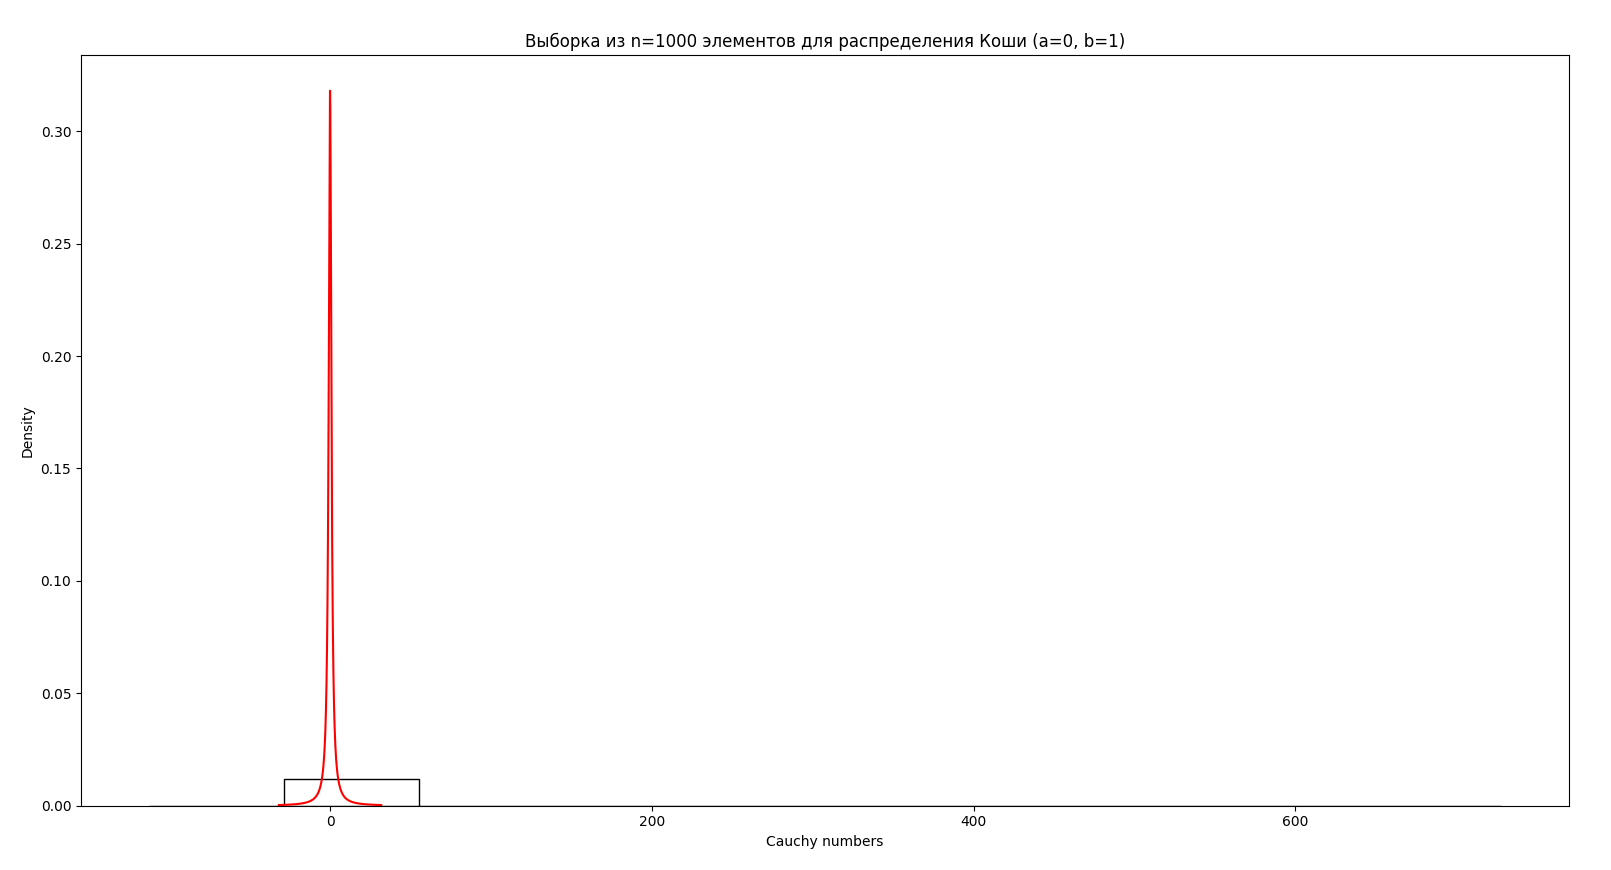
\includegraphics[scale=0.12]{resources/1_cauchy_1000.png}
	\end{tabular}
	\caption{Распределение Коши}
\end{figure}

\begin{figure}[H]
	\begin{tabular}{ccc}
		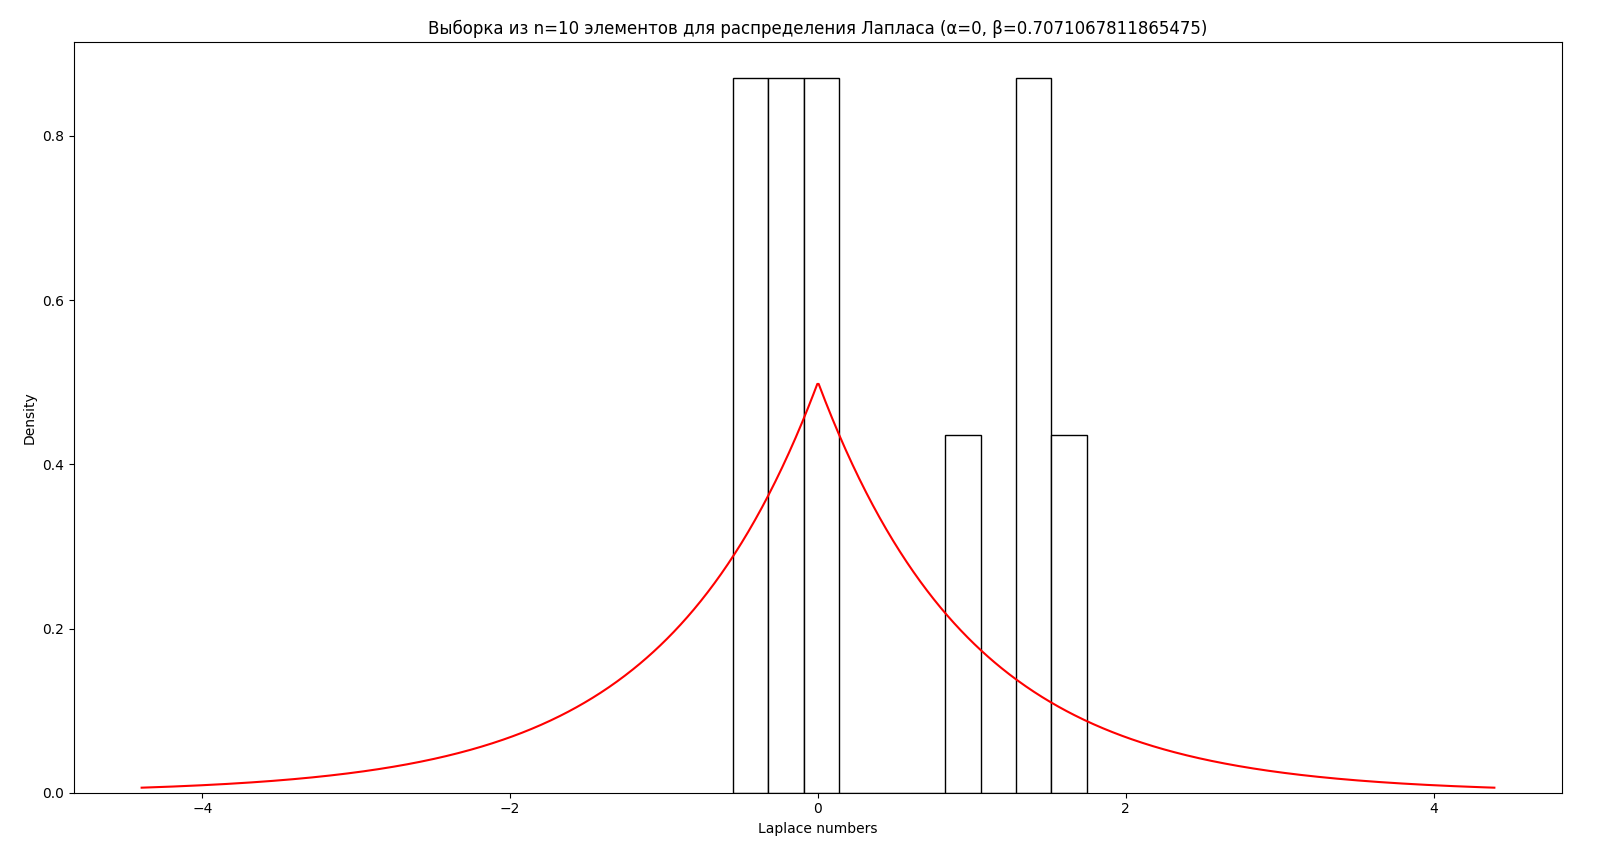
\includegraphics[scale=0.12]{resources/1_laplace_10.png}
		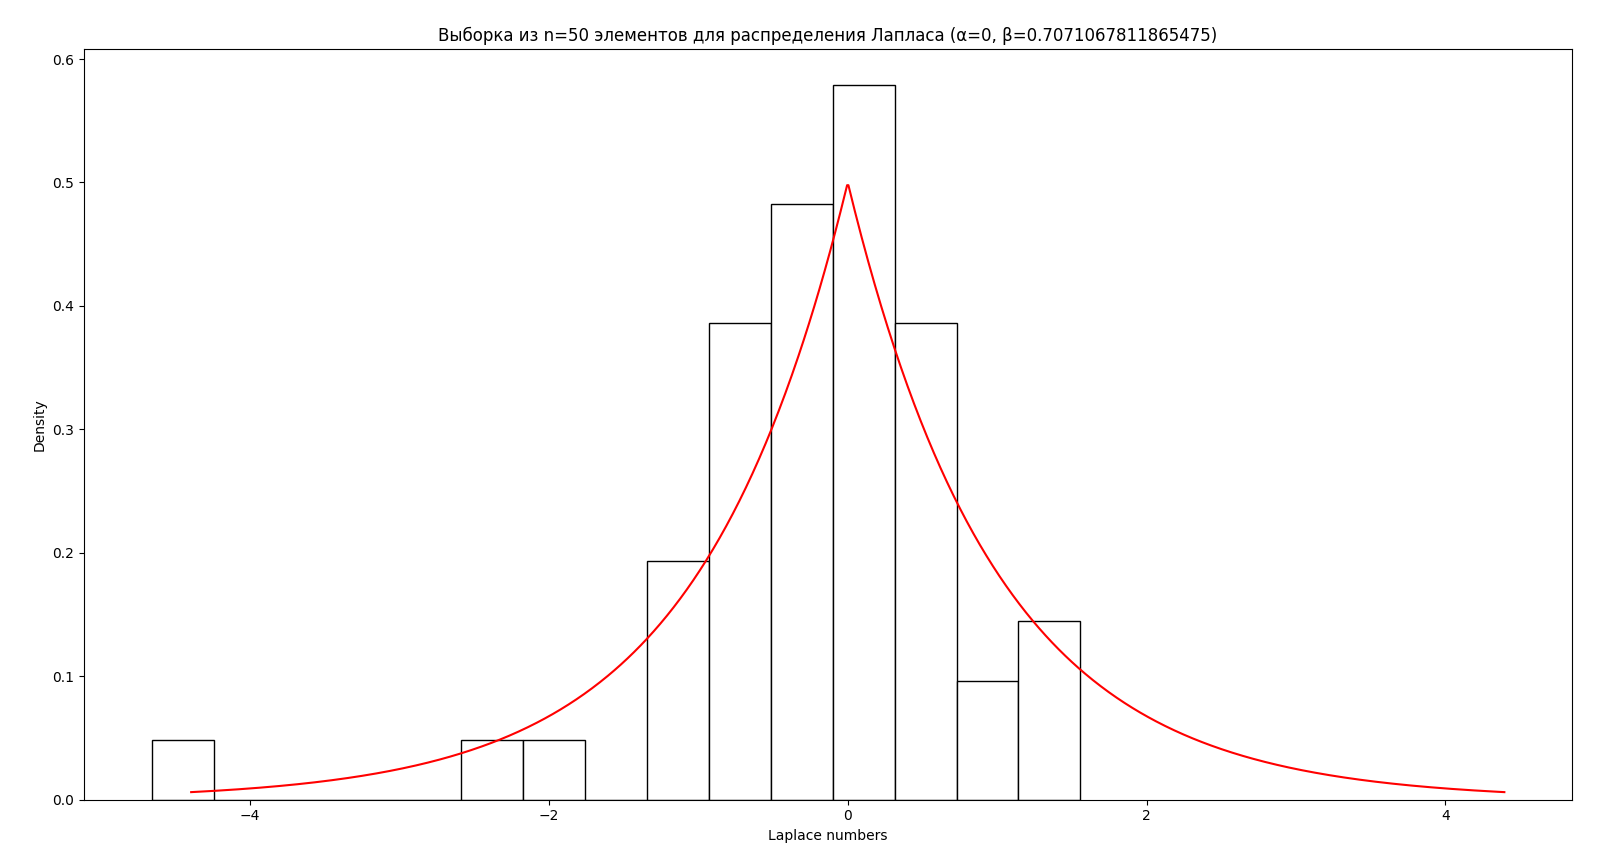
\includegraphics[scale=0.12]{resources/1_laplace_50.png}
		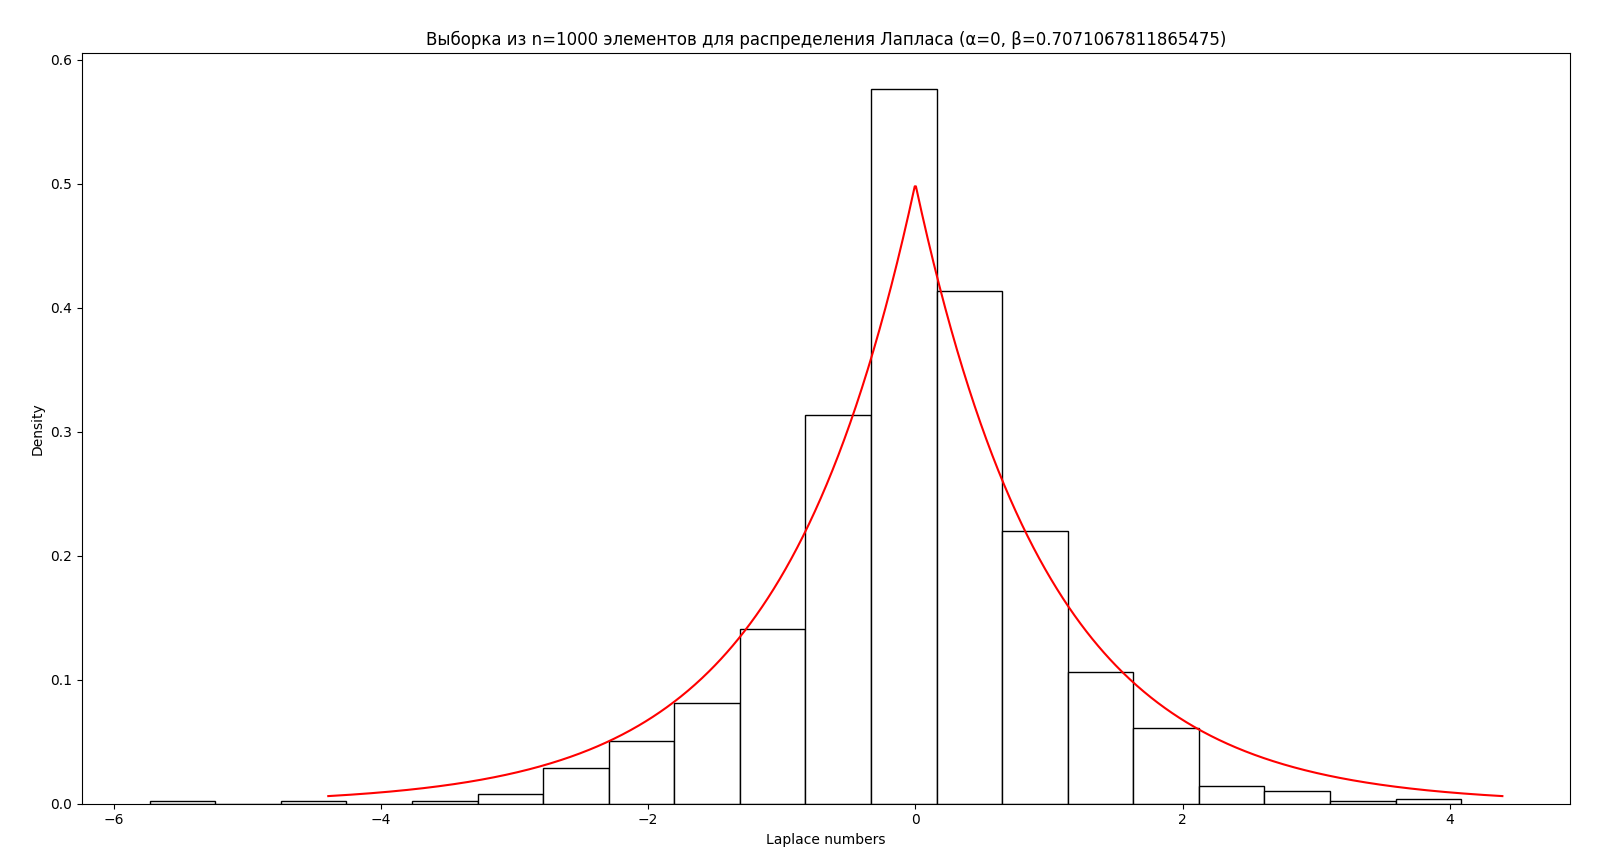
\includegraphics[scale=0.12]{resources/1_laplace_1000.png}
	\end{tabular}
	\caption{Распределение Лапласа}
\end{figure}

\begin{figure}[H]
	\begin{tabular}{ccc}
		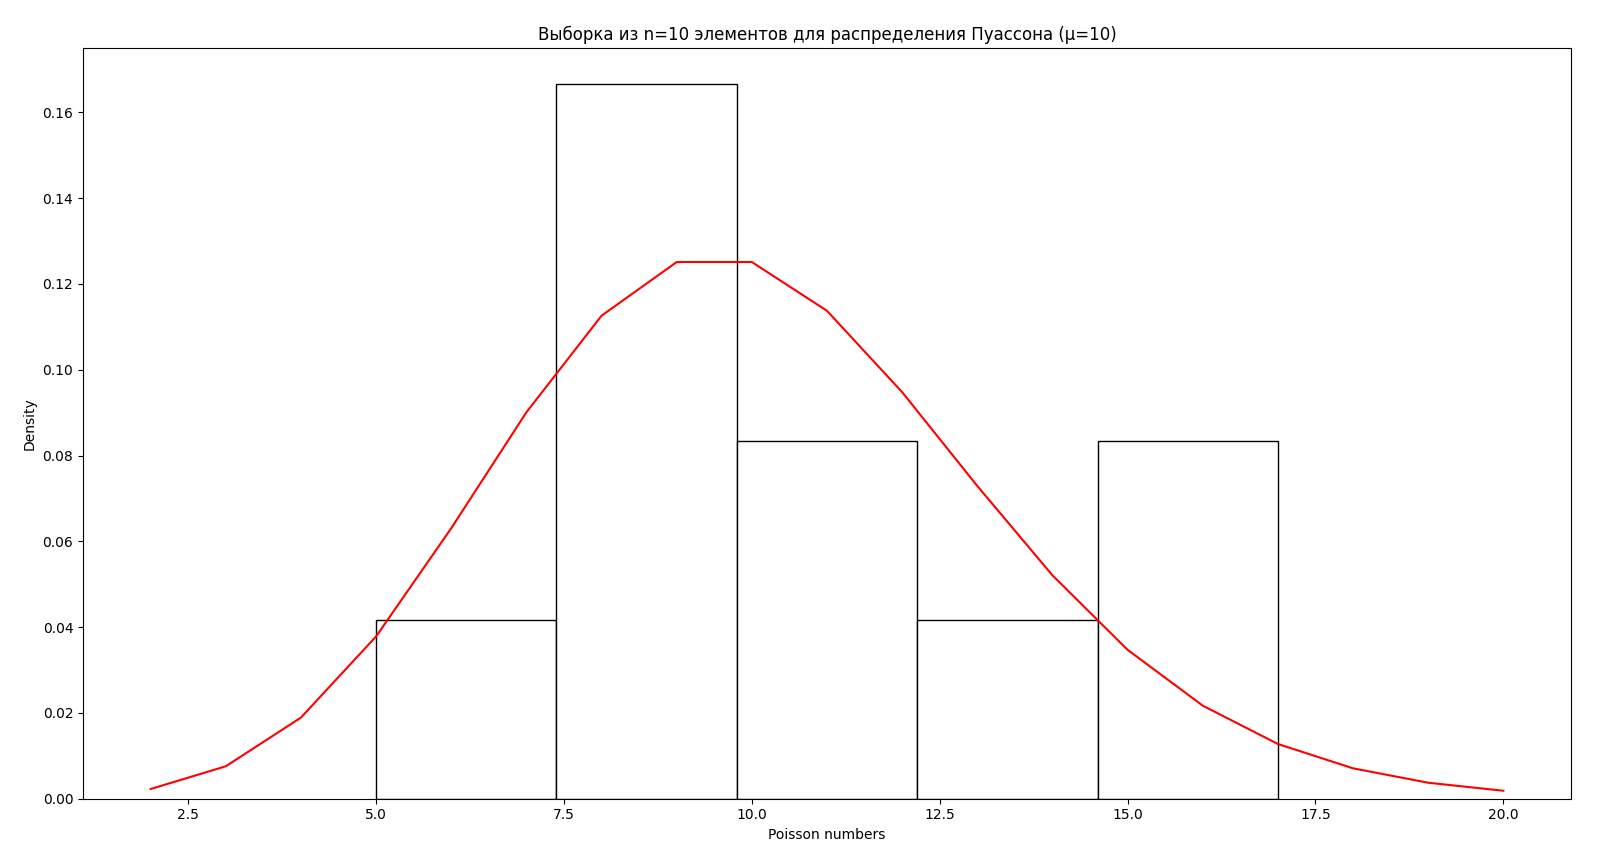
\includegraphics[scale=0.12]{resources/1_poisson_10.png}
		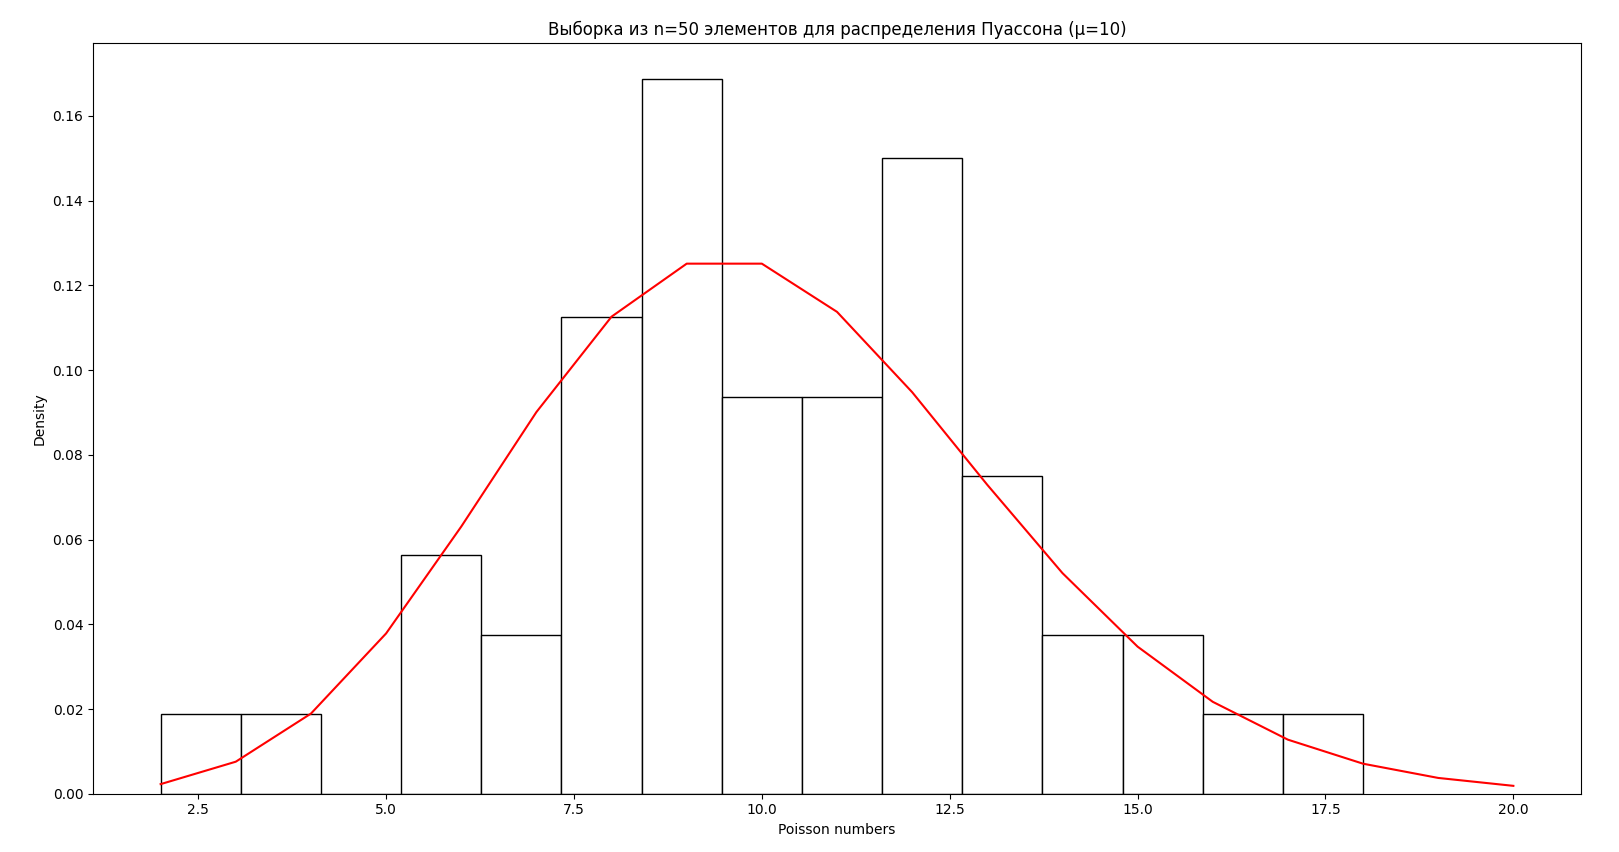
\includegraphics[scale=0.12]{resources/1_poisson_50.png}
		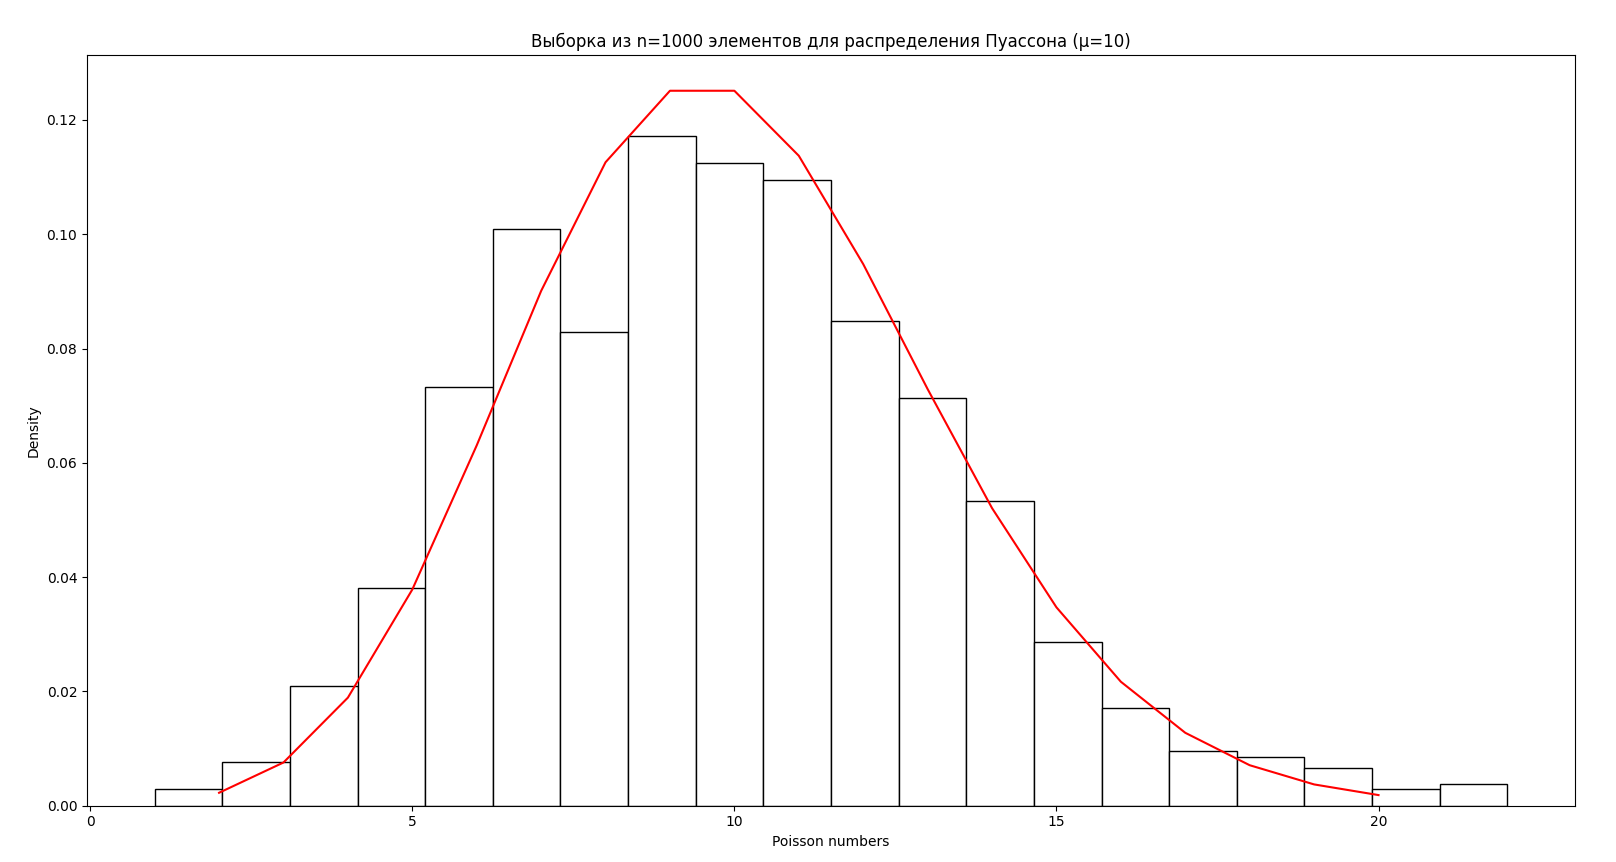
\includegraphics[scale=0.12]{resources/1_poisson_1000.png}
	\end{tabular}
	\caption{Распределение Пуассона}
\end{figure}


\begin{figure}[H]
	\begin{tabular}{ccc}
		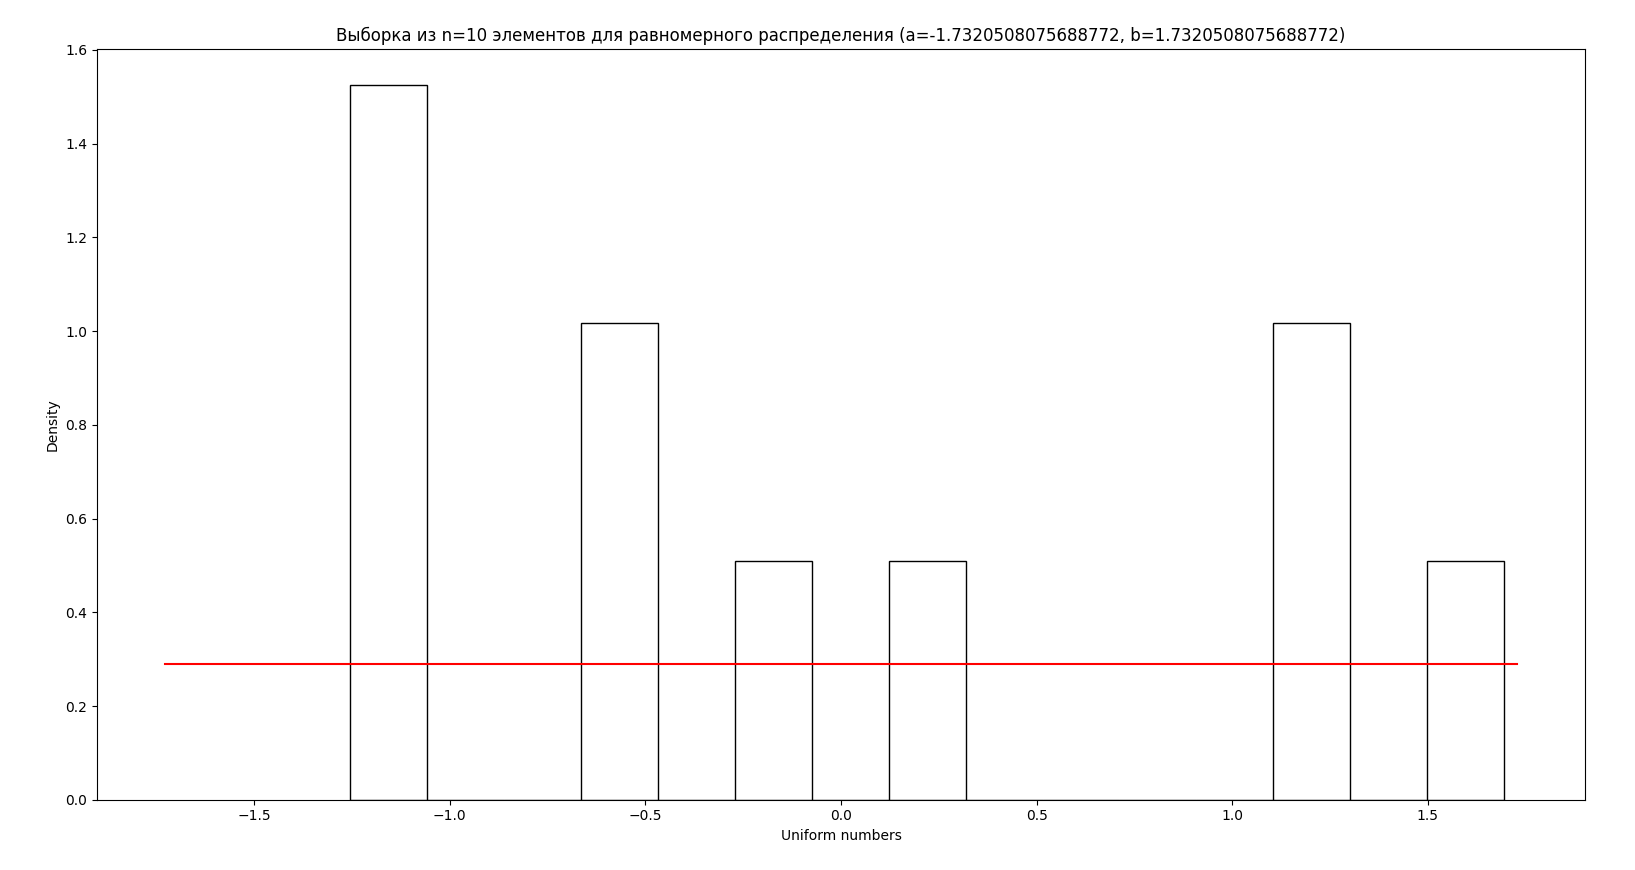
\includegraphics[scale=0.12]{resources/1_uniform_10.png}
		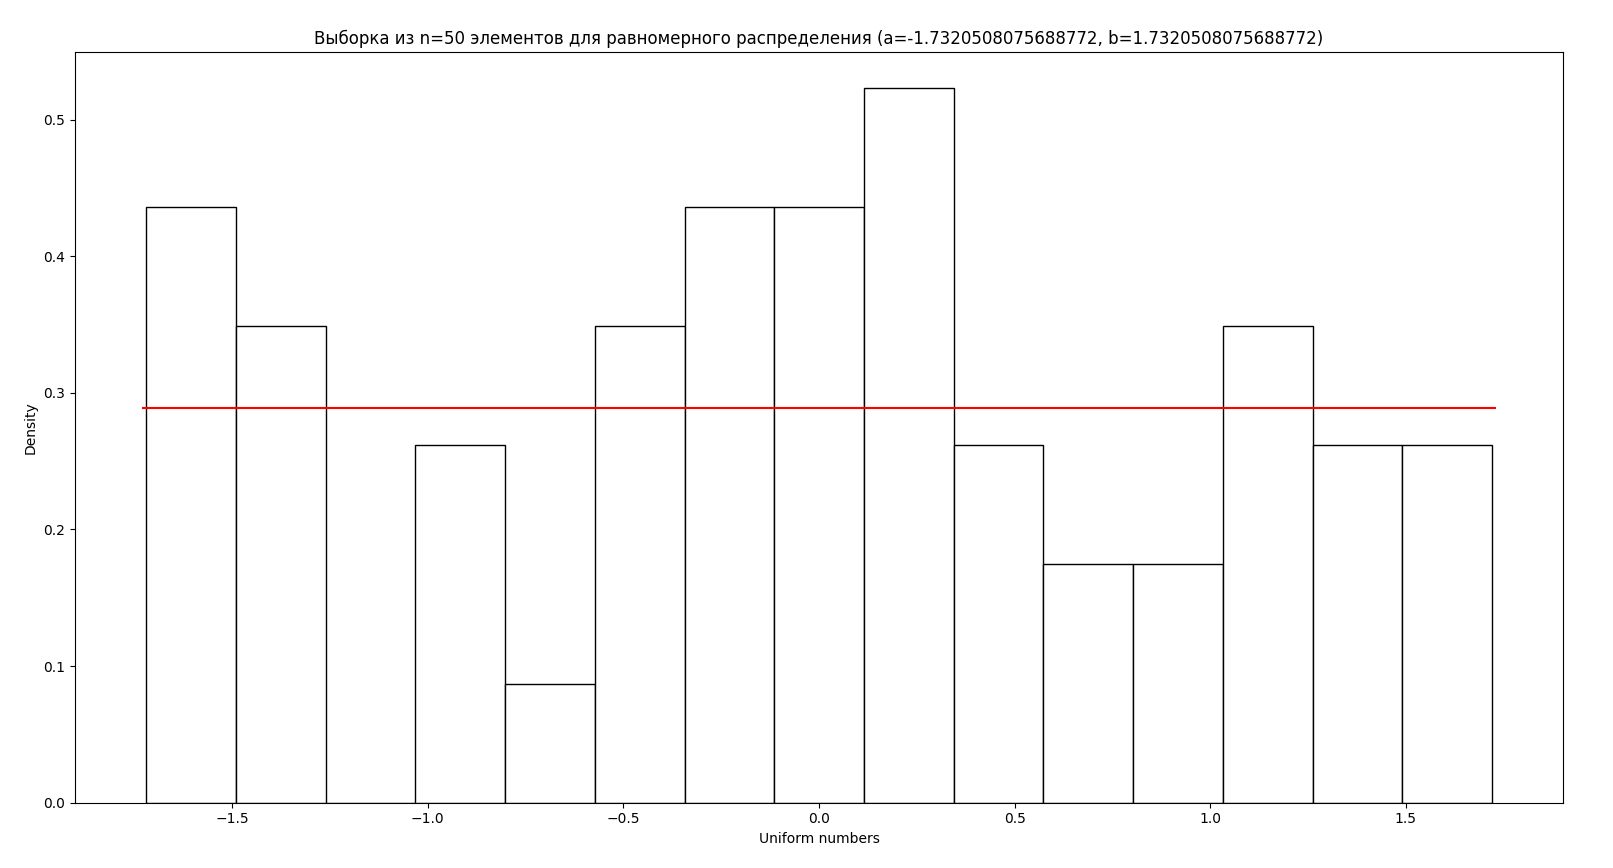
\includegraphics[scale=0.12]{resources/1_uniform_50.png}
		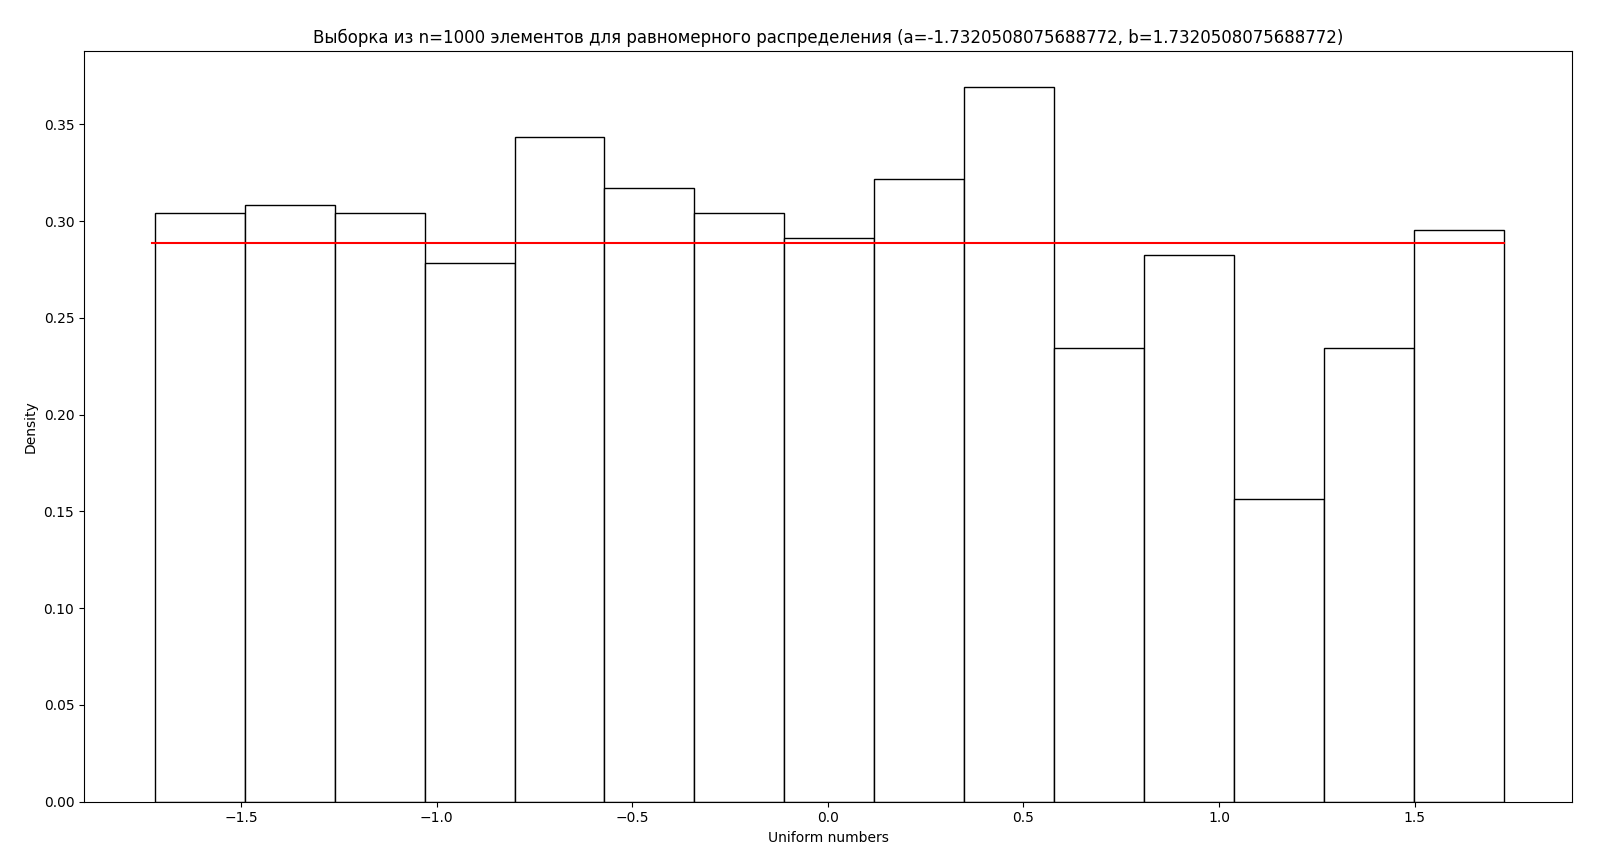
\includegraphics[scale=0.12]{resources/1_uniform_1000.png}
	\end{tabular}
	\caption{Равномерное распределение}
\end{figure}

\subsection{Характеристики положения и рассеяния}

Как было проведено округление: \\
В оценке $x = E \pm \sqrt D$ вариации подлежит первая цифра после точки.  \\
В данном случае $𝑥 = 0.0 \pm 0.1𝑘$  где, $k$ − зависит от доверительной вероятности и вида распределения (рассматривается в дальнейшем цикле лабораторных работ). \\
Округление сделано для $k = 1$.

\begin{table}[H]
	\begin{center}
		\begin{tabular}{|c||c|c|c|c|c|}
			\hline
			Gauss n = 10 & $\overline{x} $ & $med\:x$ & $z_{R}$ & $z_{Q}$ & $z_{tr}$ \\
			\hline\hline
			$E(z)$ & -0.001 & 0.120 & -0.008 & -0.001 & -0.001 \\
			\hline
			$D(z)$ & 0.107 & 0.167 & 0.205 & 0.123 & 0.120  \\
			\hline
			$E(z) \pm \sqrt{D(z)}$ & [-0.329;0.326] & [-0.289;0.529] & [-0.461;0.446] & [-0.352;0.350] & [-0.347;0.345]   \\
			\hline
			$\hat{E}(z)$  & 0 & 0 & 0 & 0 & 0  \\
			\hline\hline
			Gauss n = 100 & $\overline{x} $ & $med\:x$ & $z_{R}$ & $z_{Q}$ & $z_{tr}$ \\
			\hline\hline
			$E(z)$ & -0.002 & 0.011 & -0.010 & -0.015 & -0.001 \\
			\hline
			$D(z)$ & 0.010 & 0.016 & 0.096 & 0.013 & 0.012  \\
			\hline
			$E(z) \pm \sqrt{D(z)}$ & [-0.103;0.098] & [-0.118;0.139] & [-0.320;0.301] & [-0.129;0.098] & [-0.112;0.111]   \\
			\hline
			$\hat{E}(z)$  & 0 & 0 & 0 & 0 & 0  \\
			\hline\hline
			Gauss n = 1000 & $\overline{x} $ & $med\:x$ & $z_{R}$ & $z_{Q}$ & $z_{tr}$ \\
			\hline\hline
			$E(z)$ & 0.000 & 0.001 & 0.010 & -0.001 & 0.000 \\
			\hline
			$D(z)$ & 0.001 & 0.002 & 0.057 & 0.001 & 0.001  \\
			\hline
			$E(z) \pm \sqrt{D(z)}$ & [-0.030;0.031] & [-0.038;0.040] & [-0.229;0.249] & [-0.035;0.033] & [-0.034;0.034]   \\
			\hline
			$\hat{E}(z)$  & 0.0 & 0.0 & 0 & 0.0 & 0.0  \\
			\hline
		\end{tabular}
	\end{center}
	\caption{Характеристики положения и рассеяния нормального распределения}
\end{table} 

\begin{table}[H]
	\begin{center}
		\begin{tabular}{|c||c|c|c|c|c|}
			\hline
			Cauchy n = 10 & $\overline{x} $ & $med\:x$ & $z_{R}$ & $z_{Q}$ & $z_{tr}$ \\
			\hline\hline
			$E(z)$ & 13.257 & 0.173 & 66.059 & 0.041 & 0.006 \\
			\hline
			$D(z)$ & 95821.419 & 0.382 & 2393086.501 & 1.240 & 0.542  \\
			\hline
			$E(z) \pm \sqrt{D(z)}$ & [-296.293;322.808] & [-0.445;0.790] & [-1480.901;1613.020] & [-1.072;1.154] & [-0.730;0.742]   \\
			\hline
			$\hat{E}(z)$  & - & 0 & - & - & 0  \\
			\hline\hline
			Cauchy n = 100 & $\overline{x} $ & $med\:x$ & $z_{R}$ & $z_{Q}$ & $z_{tr}$ \\
			\hline\hline
			$E(z)$ & 0.934 & 0.018 & 43.235 & -0.020 & 0.005 \\
			\hline
			$D(z)$ & 936.934 & 0.027 & 2321693.382 & 0.055 & 0.028  \\
			\hline
			$E(z) \pm \sqrt{D(z)}$ & [-29.675;31.543] & [-0.147;0.182] & [-1480.475;1566.946] & [-0.254;0.214] & [-0.162;0.173]   \\
			\hline
			$\hat{E}(z)$  & - & 0 & - & 0 & 0  \\
			\hline\hline
			Cauchy n = 1000 & $\overline{x} $ & $med\:x$ & $z_{R}$ & $z_{Q}$ & $z_{tr}$ \\
			\hline\hline
			$E(z)$ & 2.262 & 0.004 & 1118.595 & 0.002 & 0.003 \\
			\hline
			$D(z)$ & 954.296 & 0.002 & 236247167.367 & 0.005 & 0.003  \\
			\hline
			$E(z) \pm \sqrt{D(z)}$ & [-28.630;33.153] & [-0.045;0.053] & [-14251.739;16488.929] & [-0.068;0.072] & [-0.048;0.053]   \\
			\hline
			$\hat{E}(z)$  & - & 0.0 & - & 0.0 & 0.0  \\
			\hline
		\end{tabular}
	\end{center}
	\caption{Характеристики положения и рассеяния распределения Коши}
\end{table}

\begin{table}[H]
	\begin{center}
		\begin{tabular}{|c||c|c|c|c|c|}
			\hline
			Laplace n = 10 & $\overline{x} $ & $med\:x$ & $z_{R}$ & $z_{Q}$ & $z_{tr}$ \\
			\hline\hline
			$E(z)$ & 0.009 & 0.093 & 0.004 & 0.011 & 0.010 \\
			\hline
			$D(z)$ & 0.093 & 0.074 & 0.409 & 0.092 & 0.066  \\
			\hline
			$E(z) \pm \sqrt{D(z)}$ & [-0.296;0.315] & [-0.179;0.366] & [-0.636;0.644] & [-0.293;0.314] & [-0.247;0.266]   \\
			\hline
			$\hat{E}(z)$  & 0 & 0 & 0 & 0 & 0  \\
			\hline\hline
			Laplace n = 100 & $\overline{x} $ & $med\:x$ & $z_{R}$ & $z_{Q}$ & $z_{tr}$ \\
			\hline\hline
			$E(z)$ & 0.003 & 0.008 & 0.043 & -0.014 & 0.000 \\
			\hline
			$D(z)$ & 0.010 & 0.006 & 0.381 & 0.011 & 0.007  \\
			\hline
			$E(z) \pm \sqrt{D(z)}$ & [-0.100;0.105] & [-0.070;0.086] & [-0.574;0.660] & [-0.117;0.088] & [-0.080;0.081]   \\
			\hline
			$\hat{E}(z)$  & 0 & 0.0 & 0 & 0 & 0.0  \\
			\hline\hline
			Laplace n = 1000 & $\overline{x} $ & $med\:x$ & $z_{R}$ & $z_{Q}$ & $z_{tr}$ \\
			\hline\hline
			$E(z)$ & 0.000 & 0.001 & 0.010 & -0.001 & -0.000 \\
			\hline
			$D(z)$ & 0.001 & 0.001 & 0.404 & 0.001 & 0.001  \\
			\hline
			$E(z) \pm \sqrt{D(z)}$ & [-0.031;0.032] & [-0.022;0.023] & [-0.626;0.646] & [-0.033;0.030] & [-0.025;0.025]   \\
			\hline
			$\hat{E}(z)$  & 0.0 & 0.0 & 0 & 0.0 & 0.0  \\
			\hline
		\end{tabular}
	\end{center}
	\caption{Характеристики положения и рассеяния распределения Лапласа}
\end{table} 

\begin{table}[H]
	\begin{center}
		\begin{tabular}{|c||c|c|c|c|c|}
			\hline
			Poisson n = 10 & $\overline{x} $ & $med\:x$ & $z_{R}$ & $z_{Q}$ & $z_{tr}$ \\
			\hline\hline
			$E(z)$ & 10.017 & 10.296 & 10.295 & 9.938 & 9.914 \\
			\hline
			$D(z)$ & 0.994 & 1.592 & 1.963 & 1.214 & 1.137  \\
			\hline
			$E(z) \pm \sqrt{D(z)}$ & [9.020;11.014] & [9.034;11.558] & [8.894;11.696] & [8.836;11.040] & [8.848;10.981]   \\
			\hline
			$\hat{E}(z)$  & - & - & - & - & -  \\
			\hline\hline
			Poisson n = 100 & $\overline{x} $ & $med\:x$ & $z_{R}$ & $z_{Q}$ & $z_{tr}$ \\
			\hline\hline
			$E(z)$ & 9.990 & 9.873 & 10.945 & 9.864 & 9.851 \\
			\hline
			$D(z)$ & 0.094 & 0.211 & 1.062 & 0.146 & 0.110  \\
			\hline
			$E(z) \pm \sqrt{D(z)}$ & [9.684;10.296] & [9.414;10.332] & [9.915;11.976] & [9.482;10.246] & [9.520;10.182]   \\
			\hline
			$\hat{E}(z)$  & 10 & 10 & - & 10 & 10  \\
			\hline\hline
			Poisson n = 1000 & $\overline{x} $ & $med\:x$ & $z_{R}$ & $z_{Q}$ & $z_{tr}$ \\
			\hline\hline
			$E(z)$ & 10.003 & 9.993 & 11.636 & 9.992 & 9.860 \\
			\hline
			$D(z)$ & 0.010 & 0.007 & 0.712 & 0.004 & 0.012  \\
			\hline
			$E(z) \pm \sqrt{D(z)}$ & [9.901;10.105] & [9.910;10.076] & [10.793;12.480] & [9.925;10.059] & [9.751;9.968]   \\
			\hline
			$\hat{E}(z)$  & 10 & 10.0 & - & 10.0 & 10  \\
			\hline
		\end{tabular}
	\end{center}
	\caption{Характеристики положения и рассеяния распределения Пуассона}
\end{table} 

\begin{table}[H]
	\begin{center}
		\begin{tabular}{|c||c|c|c|c|c|}
			\hline
			Uniform n = 10 & $\overline{x} $ & $med\:x$ & $z_{R}$ & $z_{Q}$ & $z_{tr}$ \\
			\hline\hline
			$E(z)$ & -0.003 & 0.151 & 0.001 & -0.008 & -0.006 \\
			\hline
			$D(z)$ & 0.097 & 0.235 & 0.044 & 0.132 & 0.157  \\
			\hline
			$E(z) \pm \sqrt{D(z)}$ & [-0.314;0.308] & [-0.333;0.636] & [-0.209;0.212] & [-0.371;0.355] & [-0.402;0.390]   \\
			\hline
			$\hat{E}(z)$  & 0 & 0 & 0 & 0 & 0  \\
			\hline\hline
			Uniform n = 100 & $\overline{x} $ & $med\:x$ & $z_{R}$ & $z_{Q}$ & $z_{tr}$ \\
			\hline\hline
			$E(z)$ & 0.001 & 0.017 & 0.001 & -0.015 & -0.001 \\
			\hline
			$D(z)$ & 0.009 & 0.027 & 0.001 & 0.014 & 0.018  \\
			\hline
			$E(z) \pm \sqrt{D(z)}$ & [-0.096;0.097] & [-0.148;0.182] & [-0.023;0.024] & [-0.133;0.102] & [-0.136;0.134]   \\
			\hline
			$\hat{E}(z)$  & 0.0 & 0 & 0.0 & 0 & 0  \\
			\hline\hline
			Uniform n = 1000 & $\overline{x} $ & $med\:x$ & $z_{R}$ & $z_{Q}$ & $z_{tr}$ \\
			\hline\hline
			$E(z)$ & 0.002 & 0.004 & 0.000 & 0.000 & 0.003 \\
			\hline
			$D(z)$ & 0.001 & 0.003 & 0.000 & 0.002 & 0.002  \\
			\hline
			$E(z) \pm \sqrt{D(z)}$ & [-0.030;0.035] & [-0.052;0.059] & [-0.002;0.003] & [-0.039;0.040] & [-0.043;0.049]   \\
			\hline
			$\hat{E}(z)$  & 0.0 & 0.0 & 0.0 & 0.0 & 0.0  \\
			\hline
		\end{tabular}
	\end{center}
	\caption{Характеристики положения и рассеяния равномерного распределения}
\end{table}

\subsection{Боксплот Тьюки}

\begin{figure}[H]
	\centering
	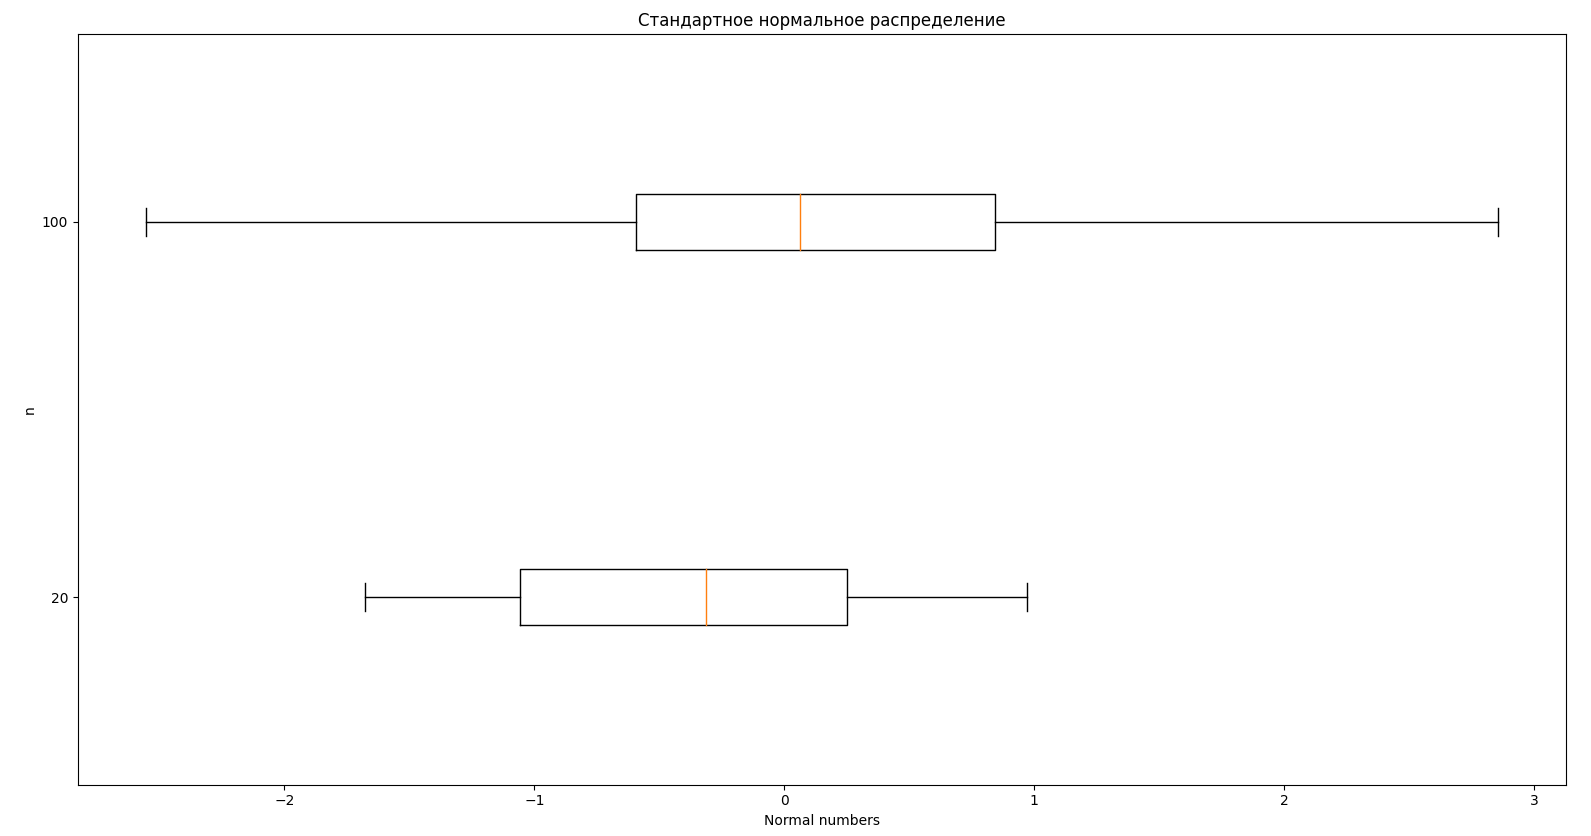
\includegraphics[scale=0.3]{resources/3_gauss.png}
	\caption{Боксплот нормального распределения}
\end{figure}

\begin{figure}[H]
	\centering
	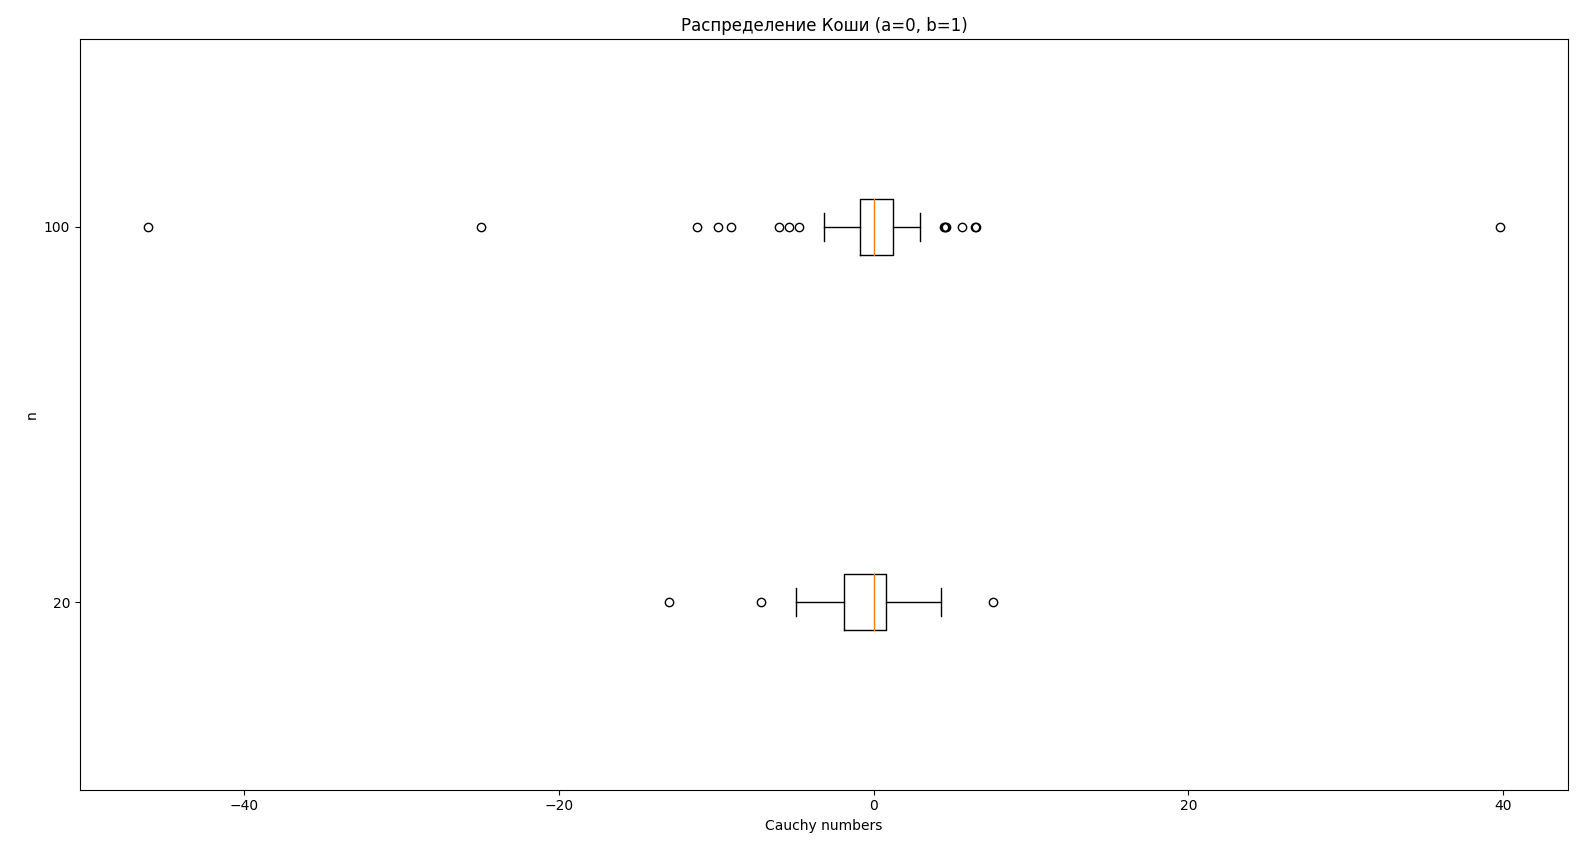
\includegraphics[scale=0.3]{resources/3_cauchy.png}
	\caption{Боксплот распределения Коши}
\end{figure}

\begin{figure}[H]
	\centering
	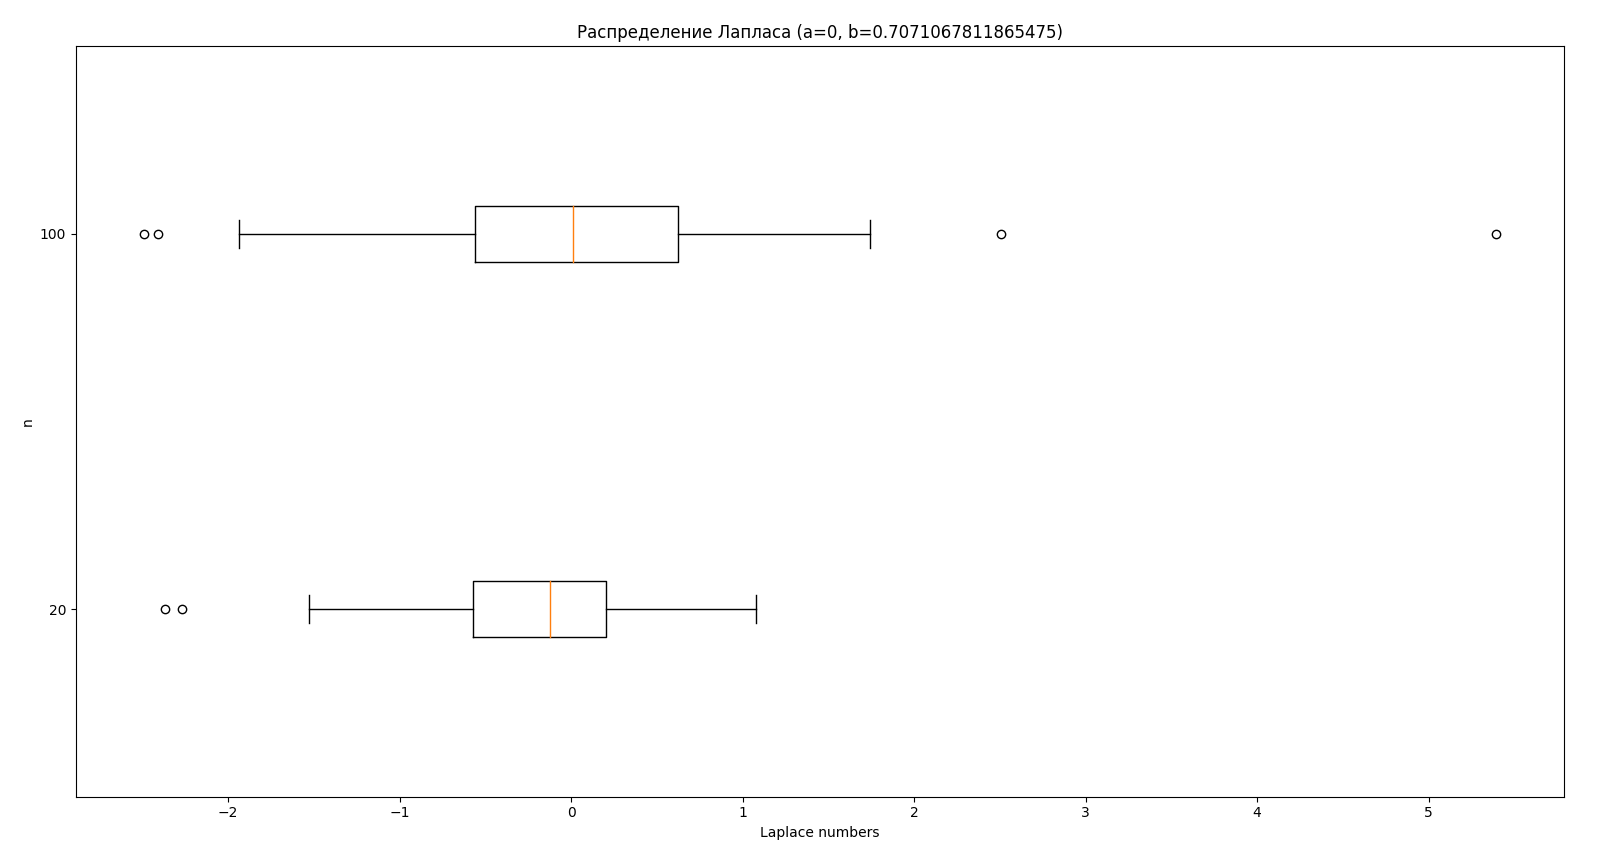
\includegraphics[scale=0.3]{resources/3_laplace.png}
	\caption{Боксплот распределения Лапласа}
\end{figure}

\begin{figure}[H]
	\centering
	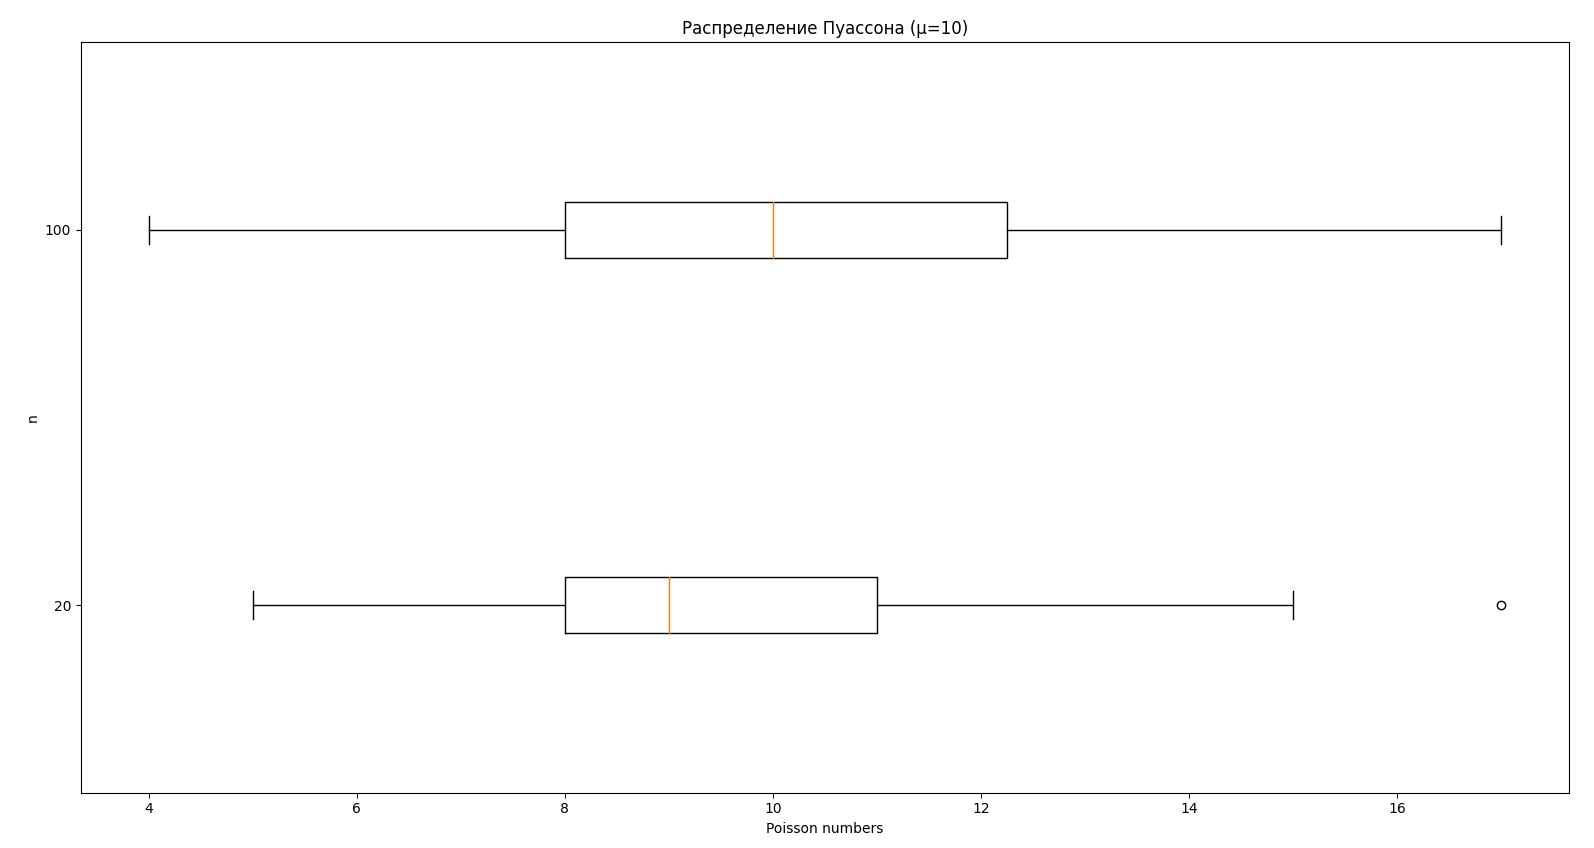
\includegraphics[scale=0.3]{resources/3_poisson.png}
	\caption{Боксплот распределения Пуассона}
\end{figure}

\begin{figure}[H]
	\centering
	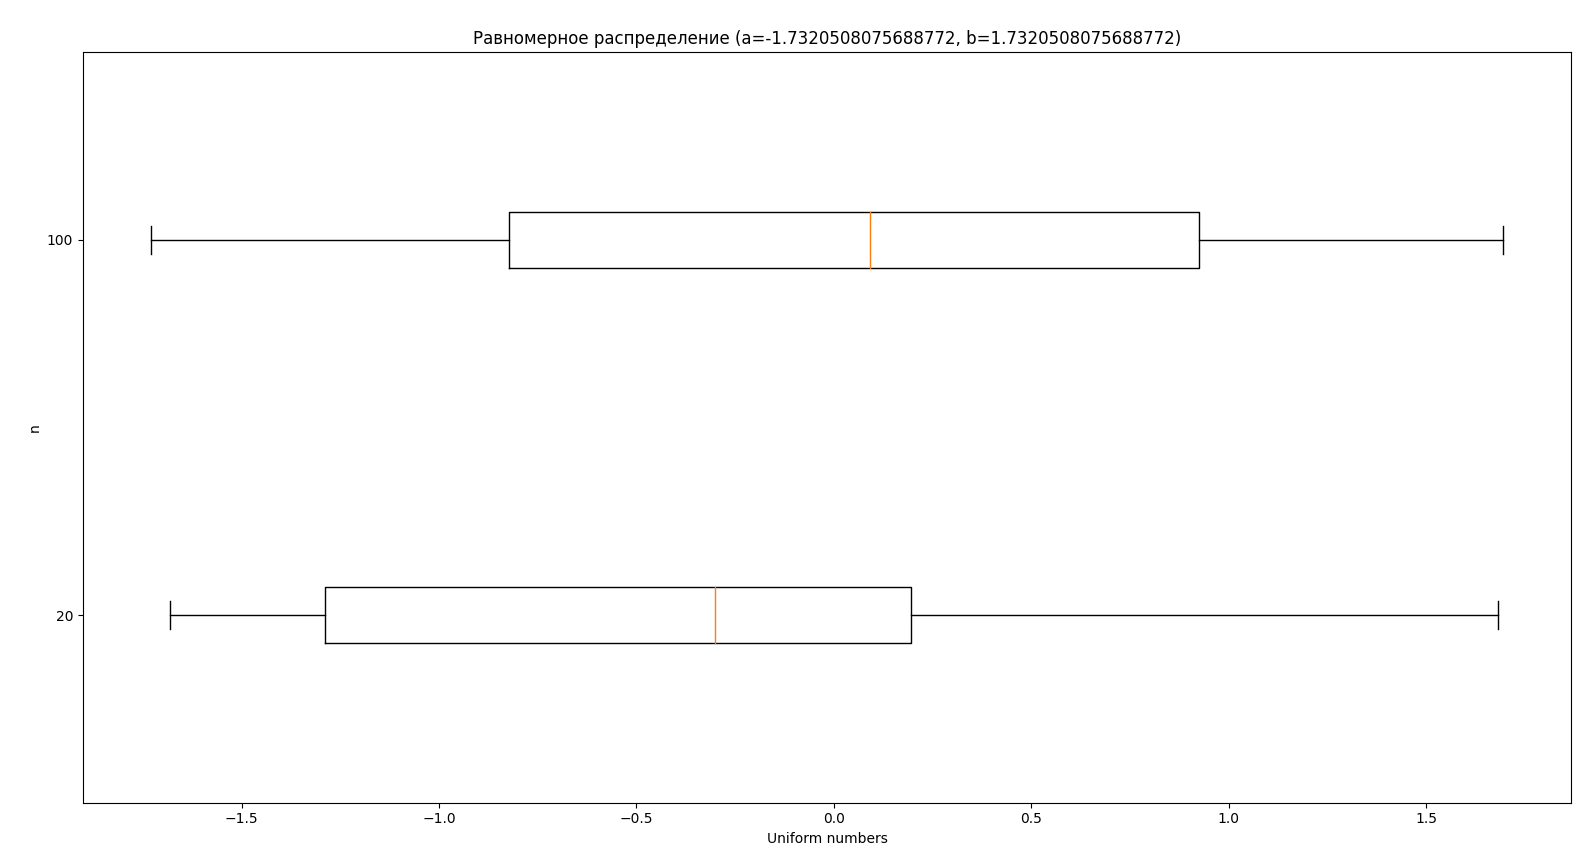
\includegraphics[scale=0.3]{resources/3_uniform.png}
	\caption{Боксплот равномерного распределения}
\end{figure}

\subsection{Доля выбросов}

\begin{table}[H]
	\begin{center}
		\begin{tabular}{|c|c|}
			\hline
			Выборка & Доля выбросов \\
			\hline\hline
			normal n=20 & 0.01\\
			\hline 
			normal n=100 & 0.02\\
			\hline
			cauchy n=20 & 0.16\\
			\hline 
			cauchy n=100 & 0.15\\
			\hline
			laplace n=20 & 0.07\\
			\hline 
			laplace n=100 & 0.07\\
			\hline
			poisson n=20 & 0.01\\
			\hline 
			poisson n=100 & 0.02\\
			\hline
			uniform n=20 & 0\\
			\hline 
			uniform n=100 & 0\\
			\hline
		\end{tabular}
	\end{center}
	\caption{Доля выбросов}
\end{table}

\subsection{Теоретическая вероятность выбросов}

\begin{table}[H]
	\begin{center}
		\begin{tabular}{|c|c|c|c|c|c|}
			\hline 
			Распределение & $Q_{1}^{T}$ & $Q_{3}^{T}$ & $X_{1}^{T}$ & $X_{2}^{T}$ & $P_{B}^{T}$ \\
			\hline\hline 
			Нормальное распределение & -0.674 & 0.674  & -2.698  & 2.698 & 0.007 \\
			\hline
			Распределение Коши & -1 & 1 &-4  &4 &0.156 \\
			\hline
			Распределение Лапласа & -0.490 & 0.490 &-1.961  &1.961 &0.063 \\
			\hline
			Распределение Пуассона & 8 & 12  & 2  & 18 & 0.008 \\
			\hline
			Равномерное распределение & -0.866 & 0.866  & -3.464  & 3.464 & 0 \\
			\hline
		\end{tabular}
	\end{center}
	\caption{Теоретическая вероятность выбросов}
\end{table}

\subsection{Эмпирическая функция распределения}

\begin{figure}[H]
	\begin{tabular}{ccc}
		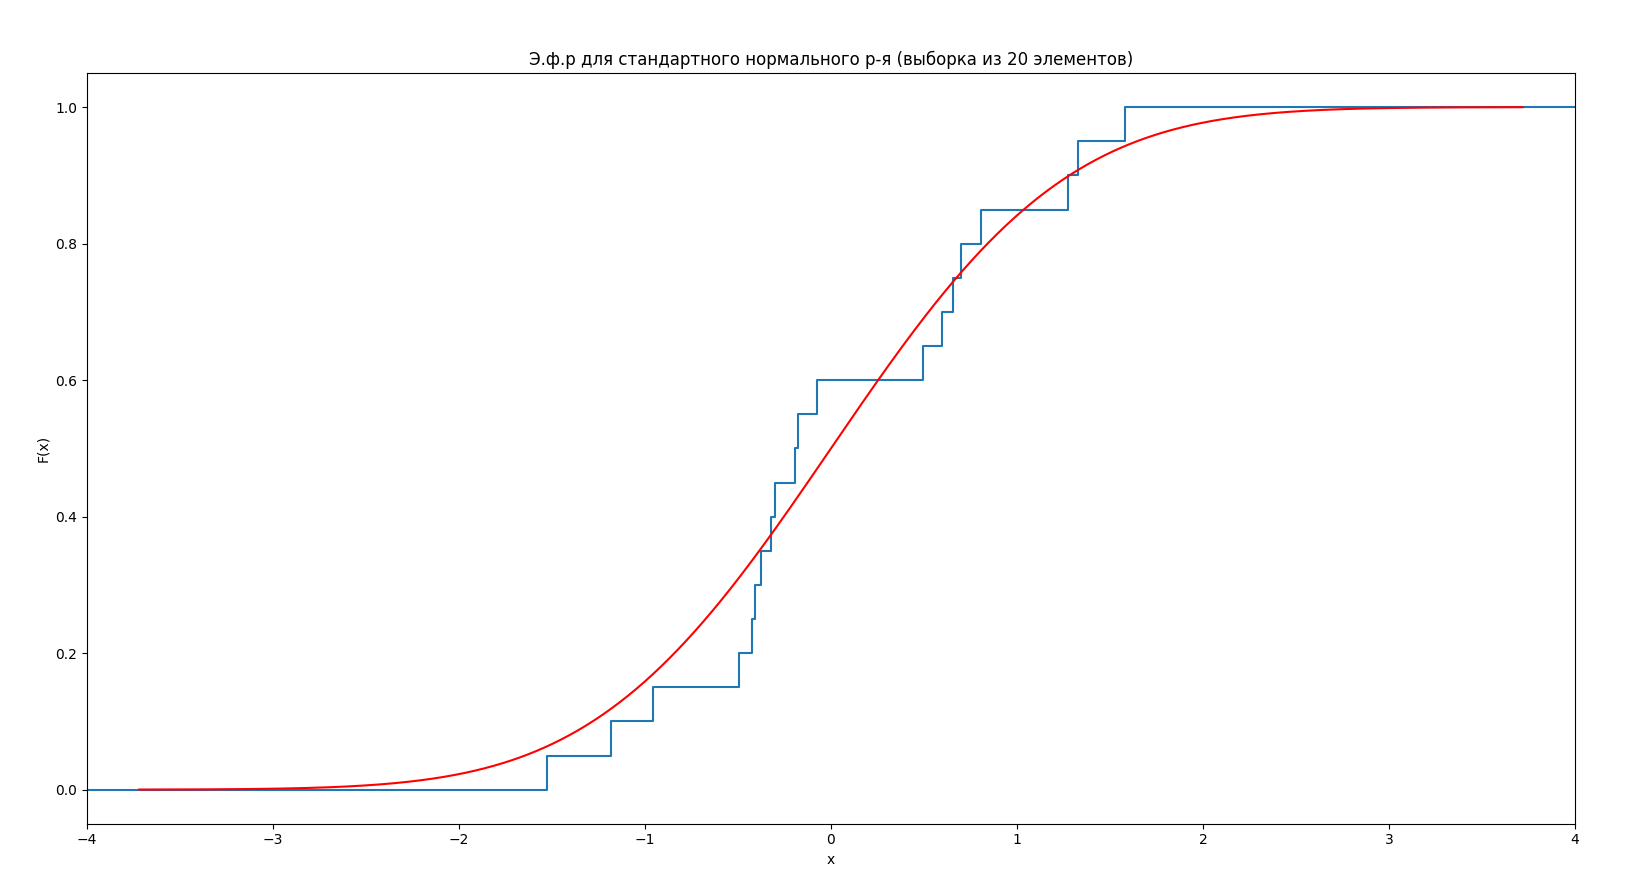
\includegraphics[scale=0.14]{resources/4_gauss_20.png}
		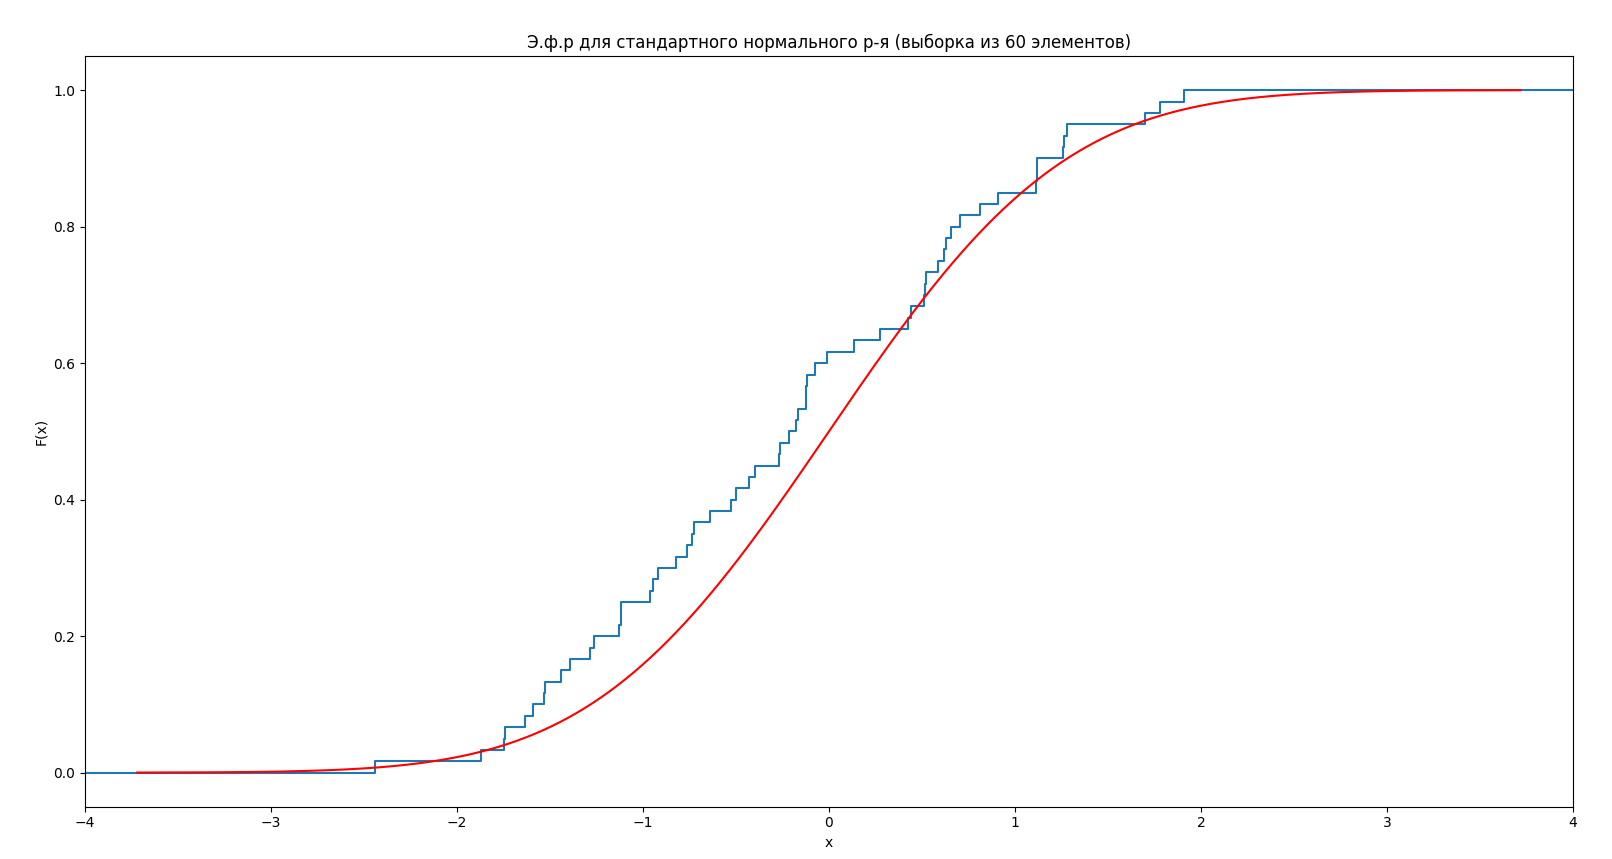
\includegraphics[scale=0.14]{resources/4_gauss_60.png}
		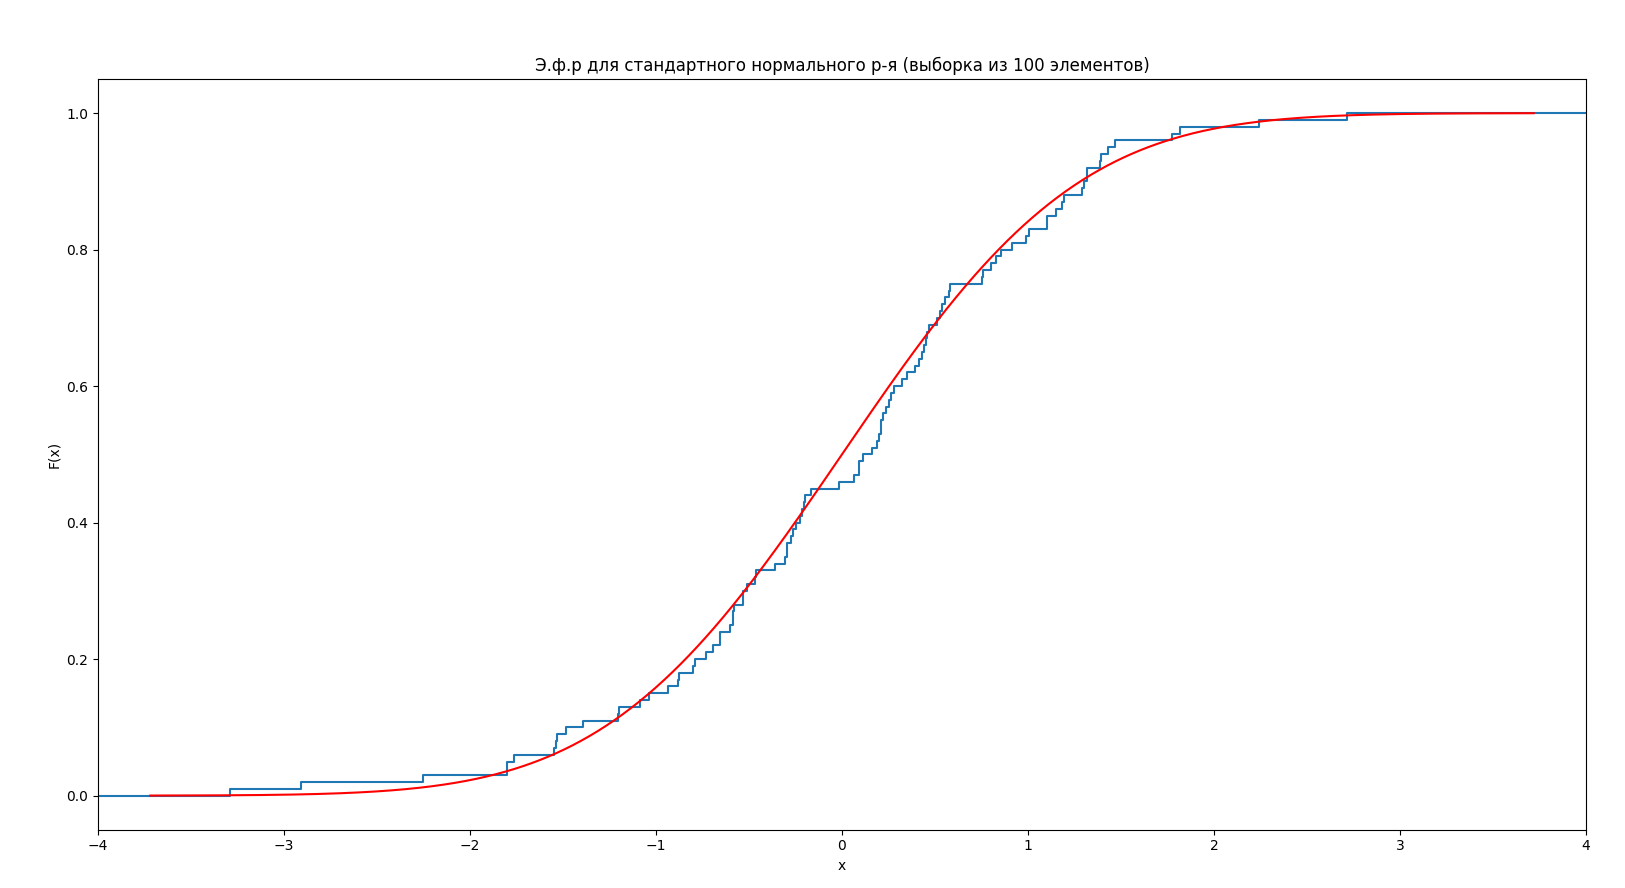
\includegraphics[scale=0.14]{resources/4_gauss_100.png}
	\end{tabular}
	\text{\tab \tab \tab n=20 \tab \tab \tab \tab \tab n=60 \tab \tab \tab \tab \tab n=100 \tab \tab }
	\caption{Нормальное распределение}
\end{figure}

\begin{figure}[H]
	\begin{tabular}{ccc}
		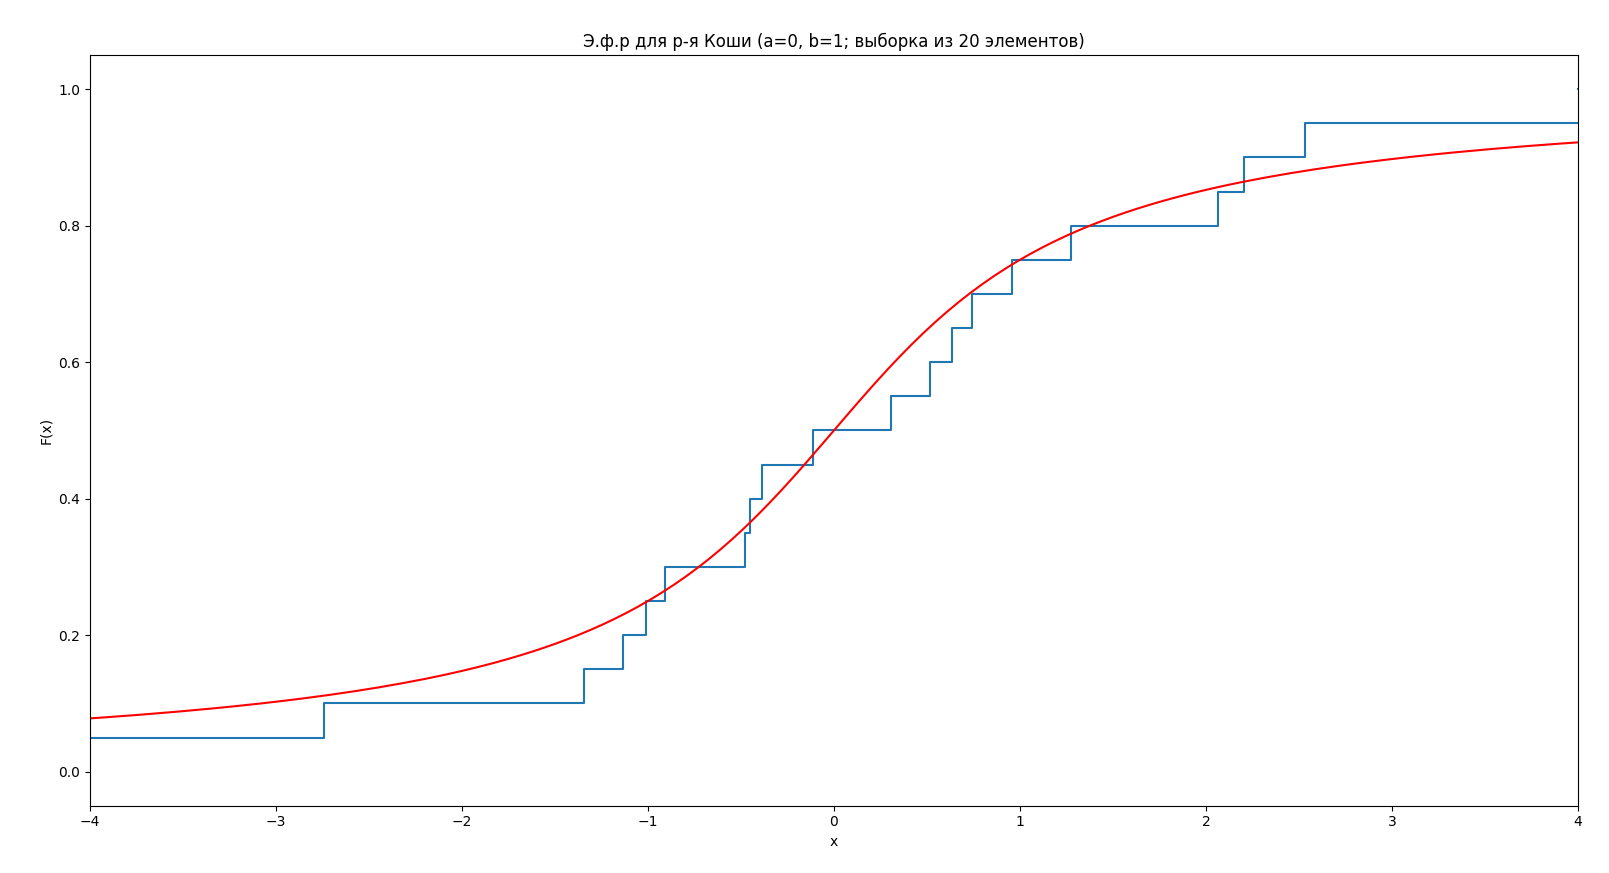
\includegraphics[scale=0.14]{resources/4_cauchy_20.png}
		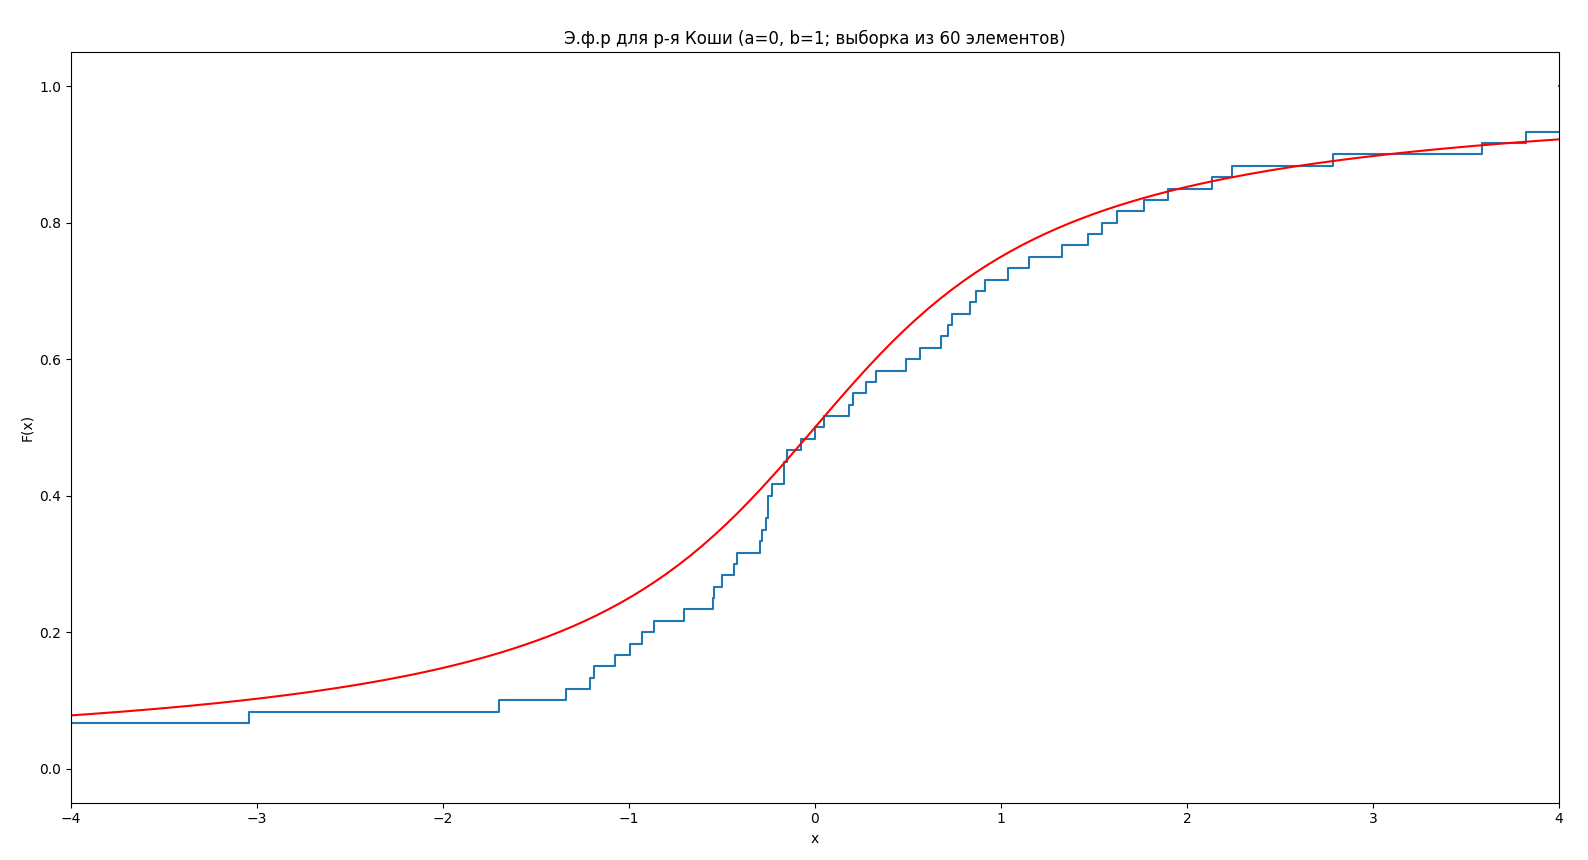
\includegraphics[scale=0.14]{resources/4_cauchy_60.png}
		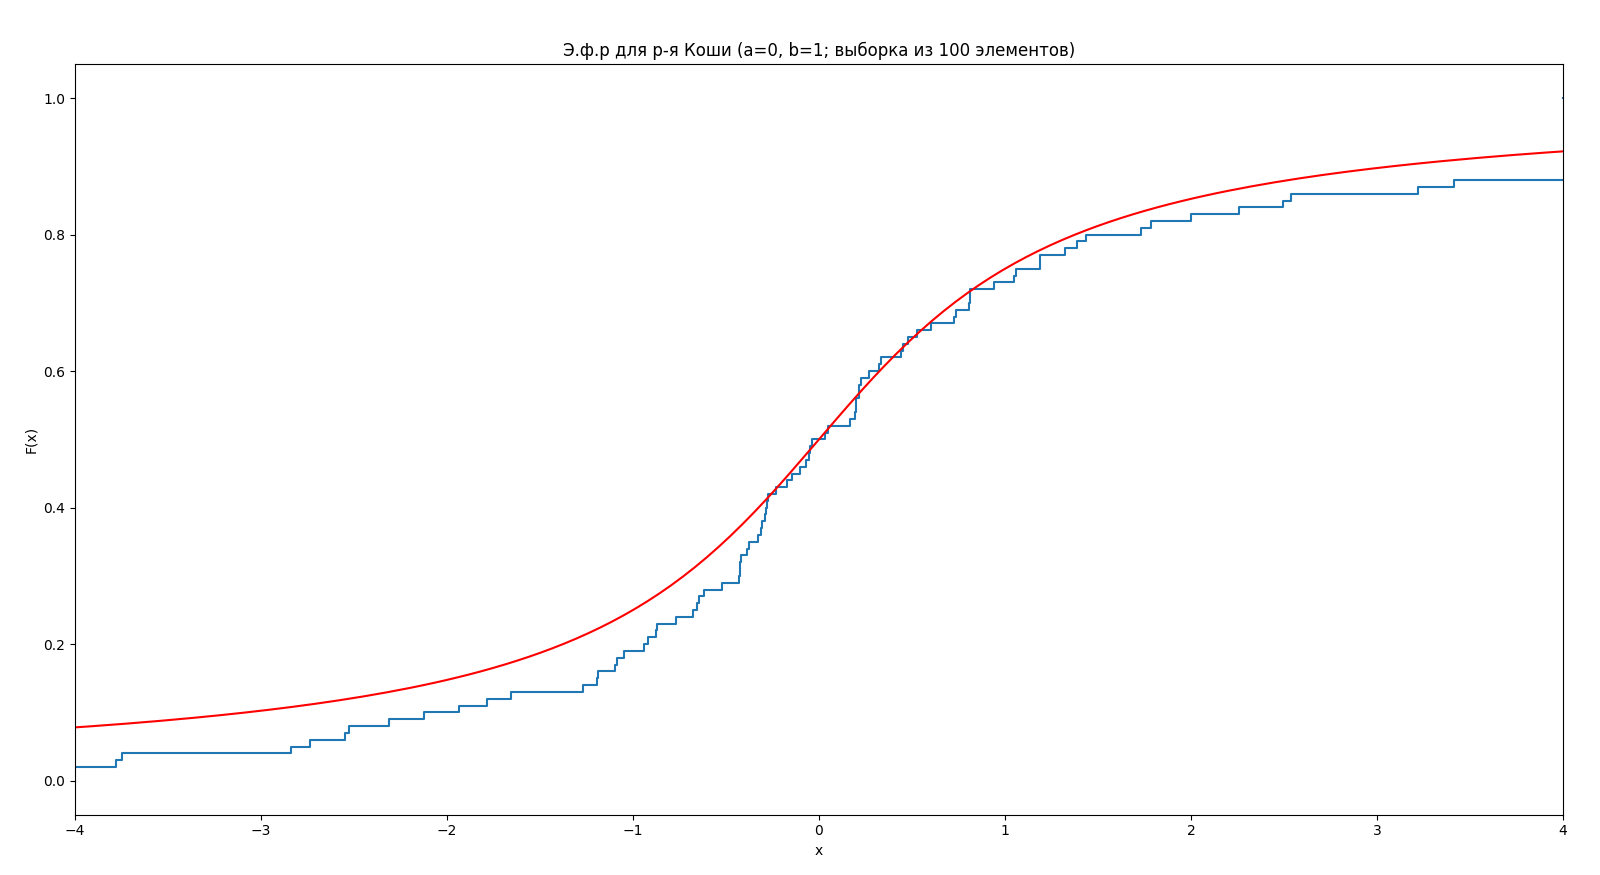
\includegraphics[scale=0.14]{resources/4_cauchy_100.png}
	\end{tabular}
	\text{\tab \tab \tab n=20 \tab \tab \tab \tab \tab n=60 \tab \tab \tab \tab \tab n=100 \tab \tab }
	\caption{Распределение Коши}
\end{figure}

\begin{figure}[H]
	\begin{tabular}{ccc}
		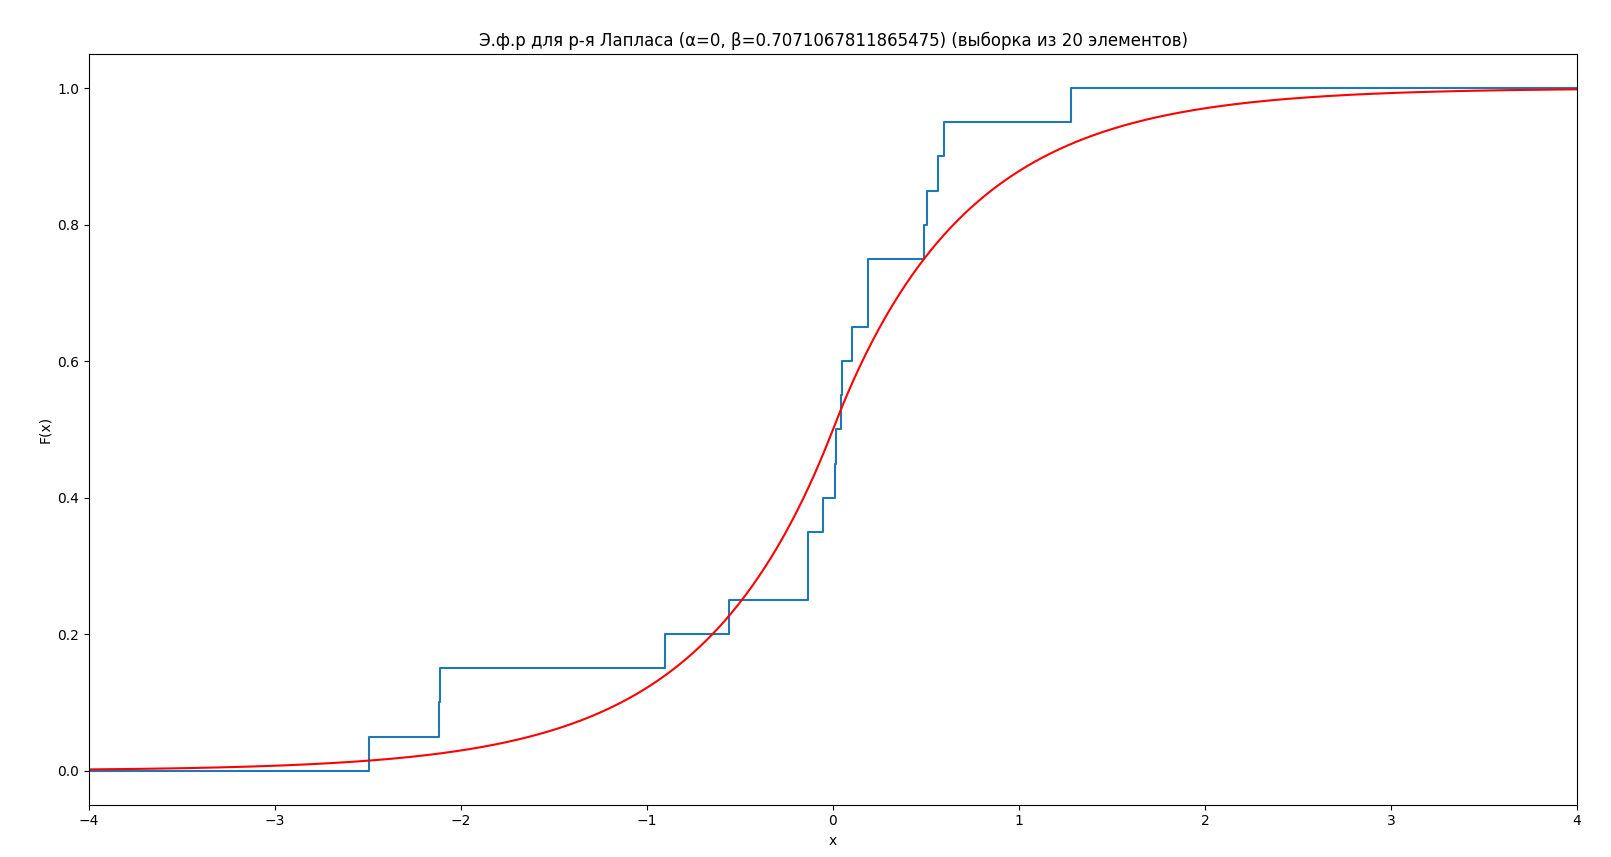
\includegraphics[scale=0.14]{resources/4_laplace_20.png}
		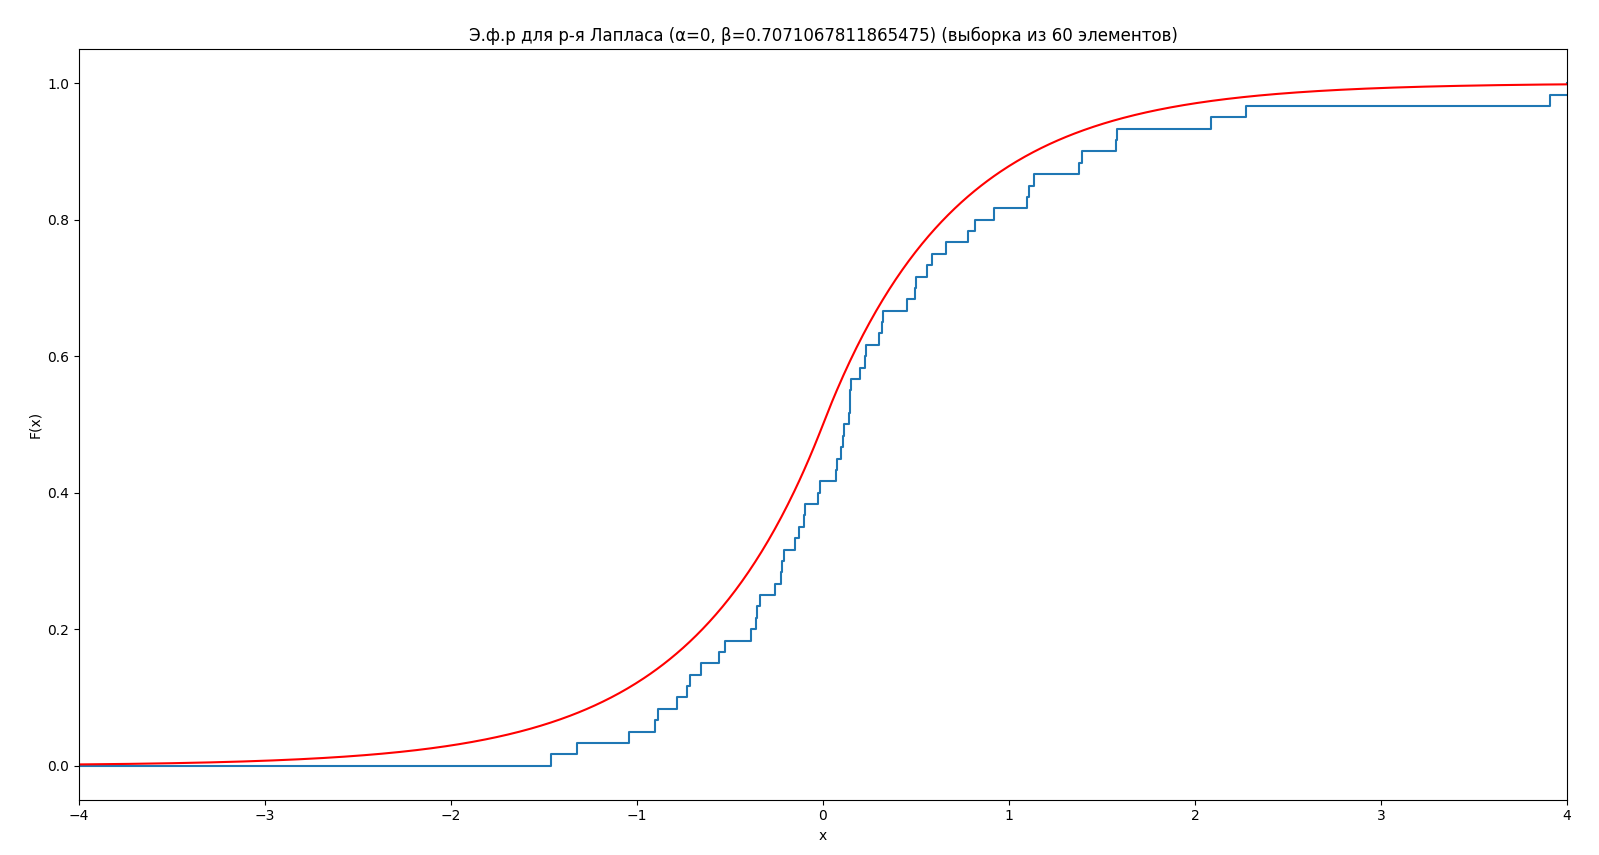
\includegraphics[scale=0.14]{resources/4_laplace_60.png}
		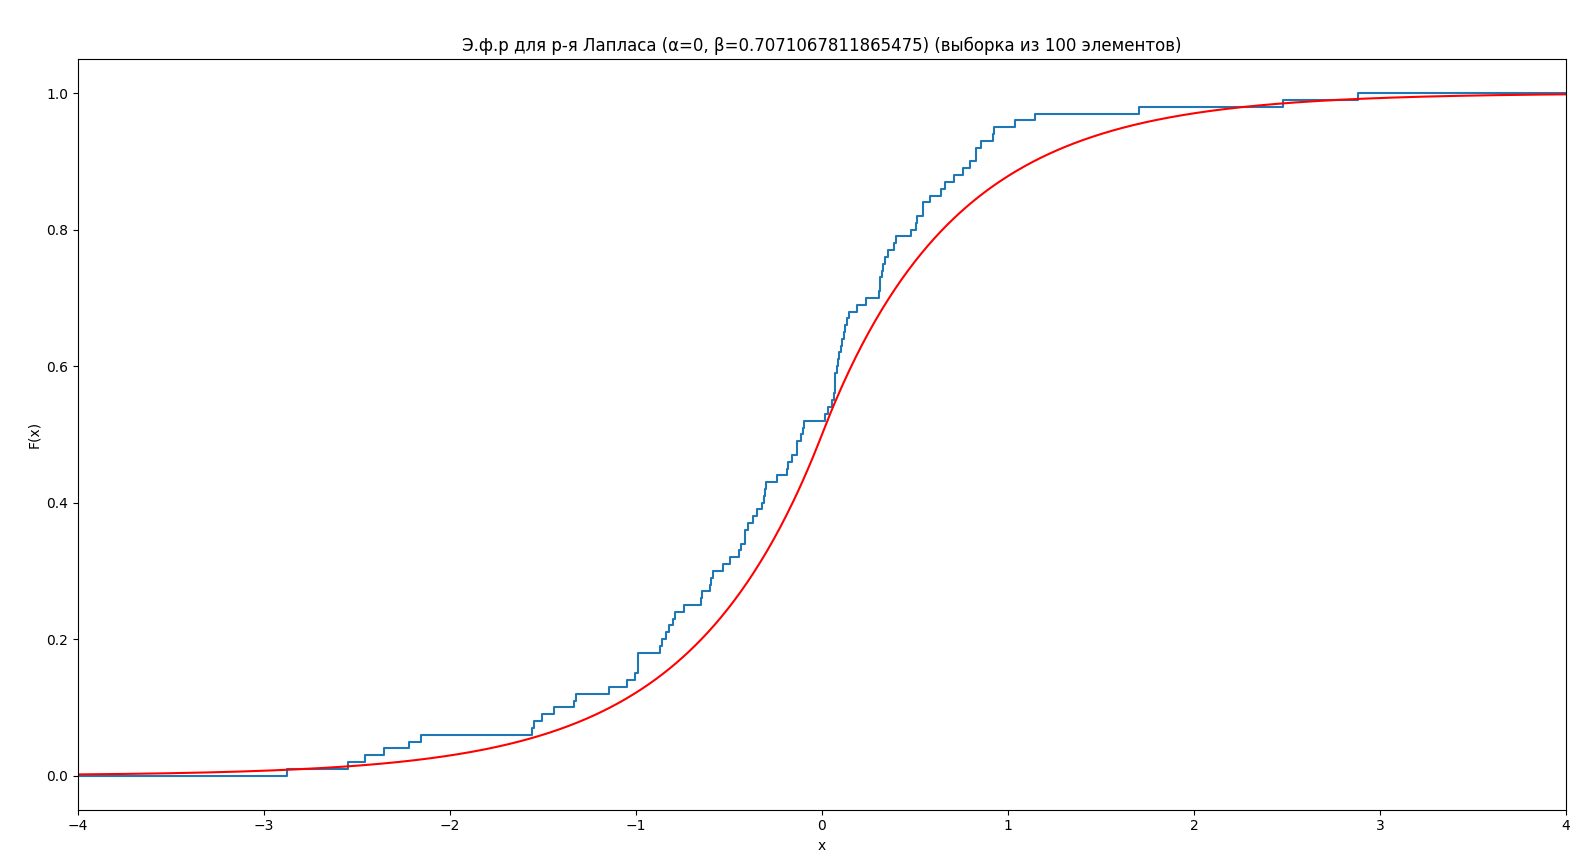
\includegraphics[scale=0.14]{resources/4_laplace_100.png}
	\end{tabular}
	\text{\tab \tab \tab n=20 \tab \tab \tab \tab \tab n=60 \tab \tab \tab \tab \tab n=100 \tab \tab }
	\caption{Распределение Лапласа}
\end{figure}

\begin{figure}[H]
	\begin{tabular}{ccc}
		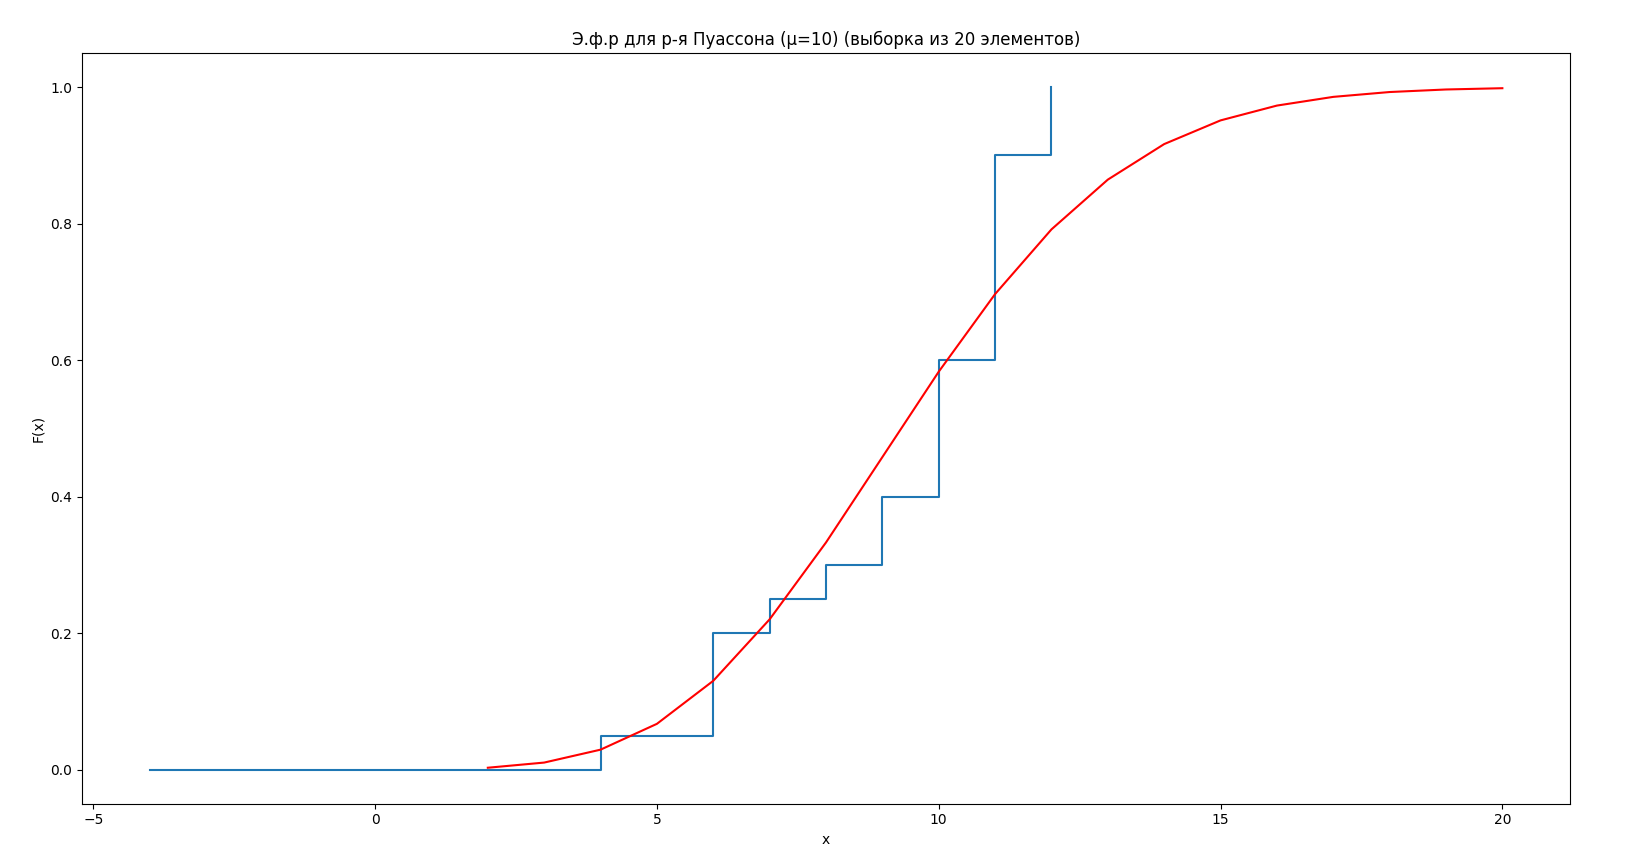
\includegraphics[scale=0.14]{resources/4_poisson_20.png}
		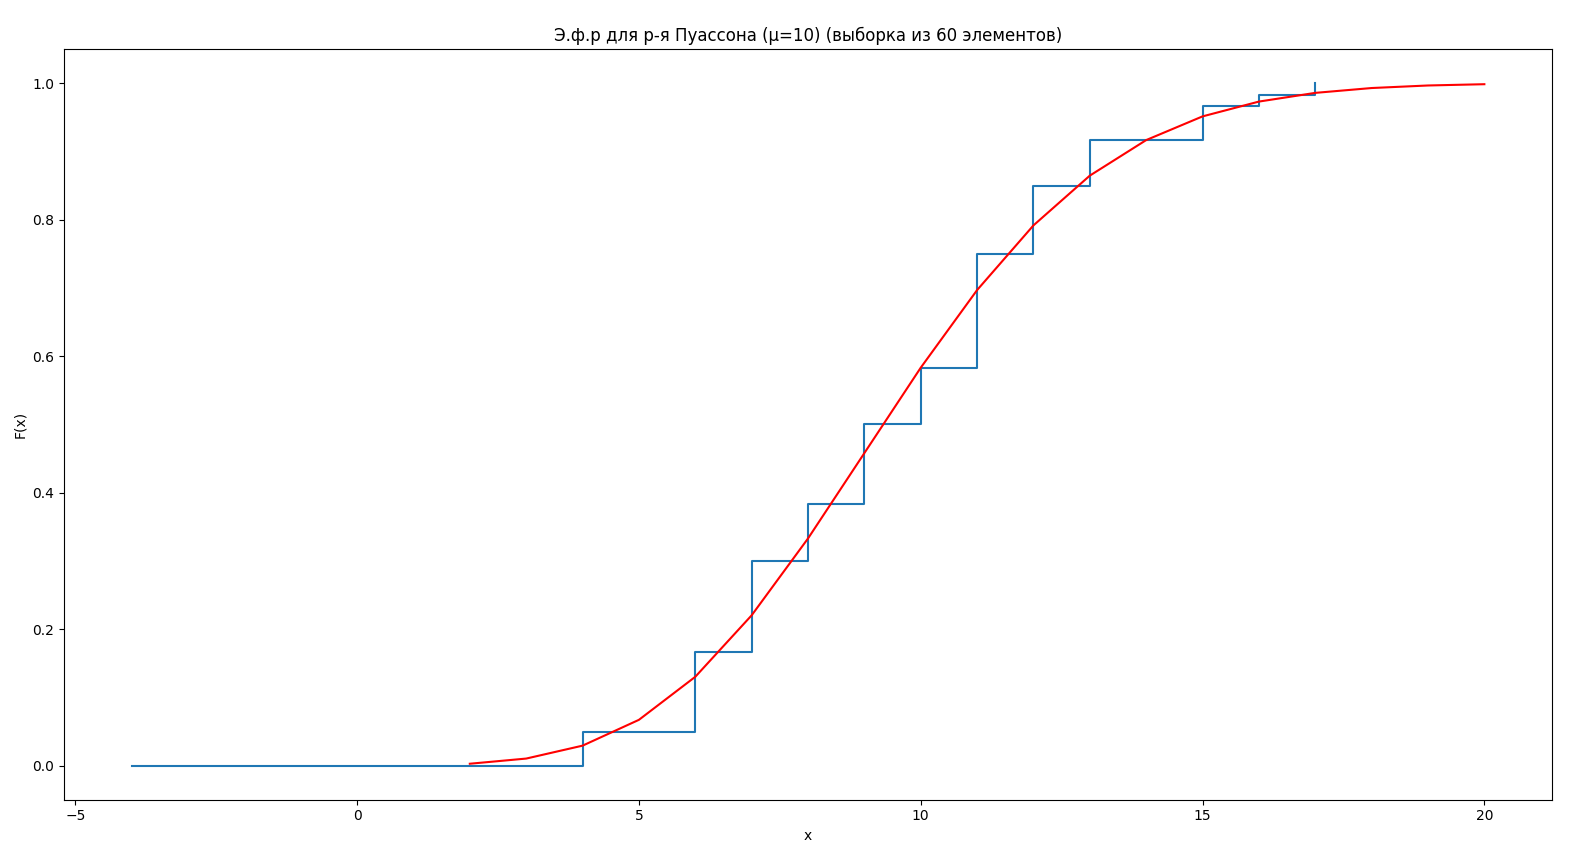
\includegraphics[scale=0.14]{resources/4_poisson_60.png}
		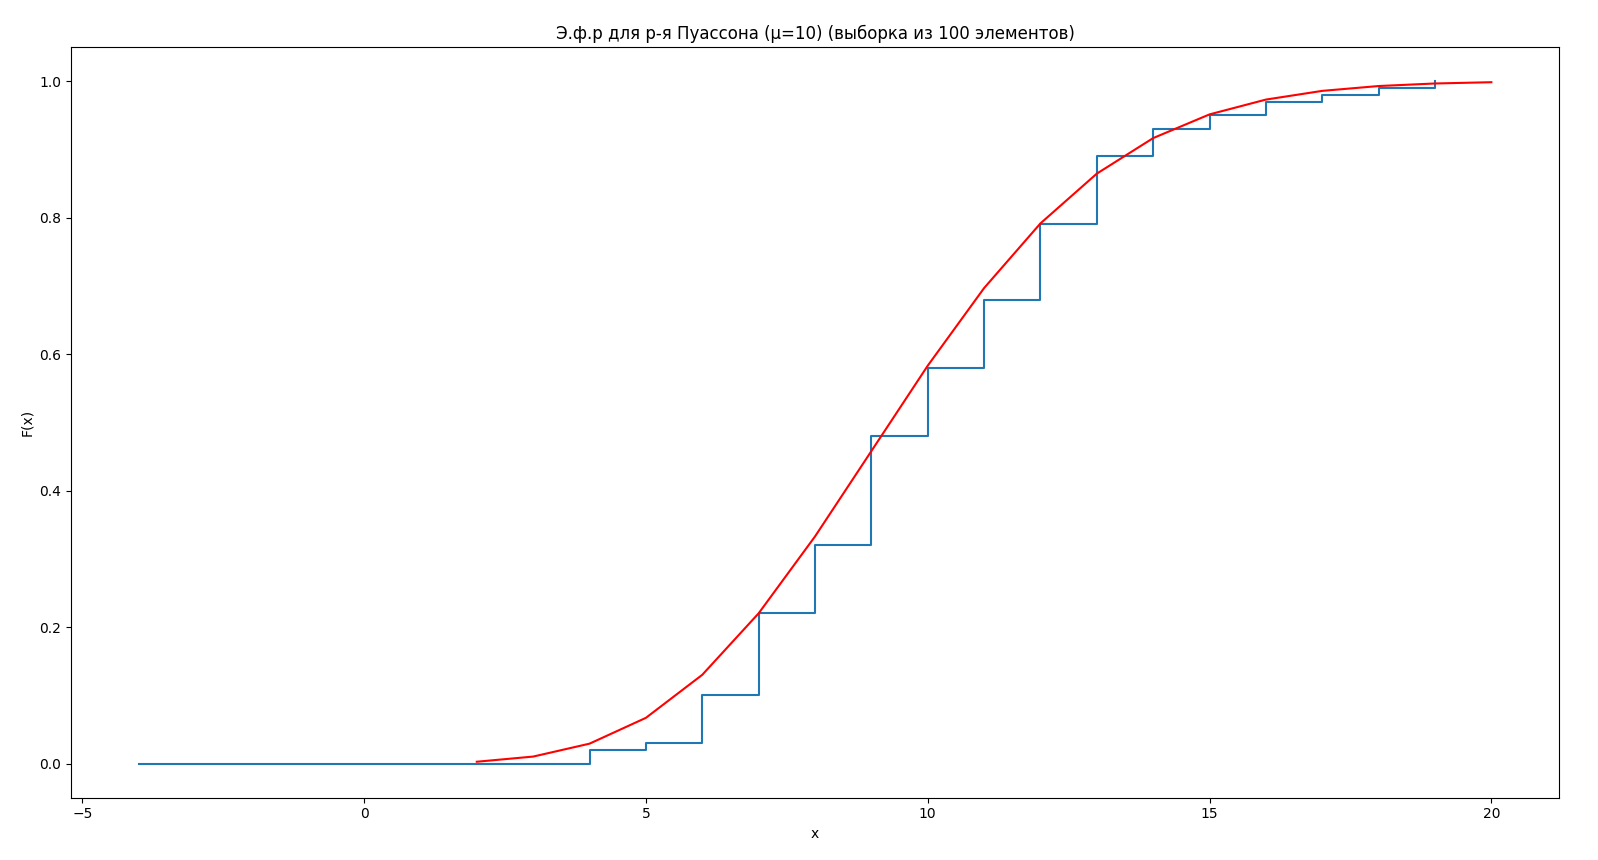
\includegraphics[scale=0.14]{resources/4_poisson_100.png}
	\end{tabular}
	\text{\tab \tab \tab n=20 \tab \tab \tab \tab \tab n=60 \tab \tab \tab \tab \tab n=100 \tab \tab }
	\caption{Распределение Пуассона}
\end{figure}


\begin{figure}[H]
	\begin{tabular}{ccc}
		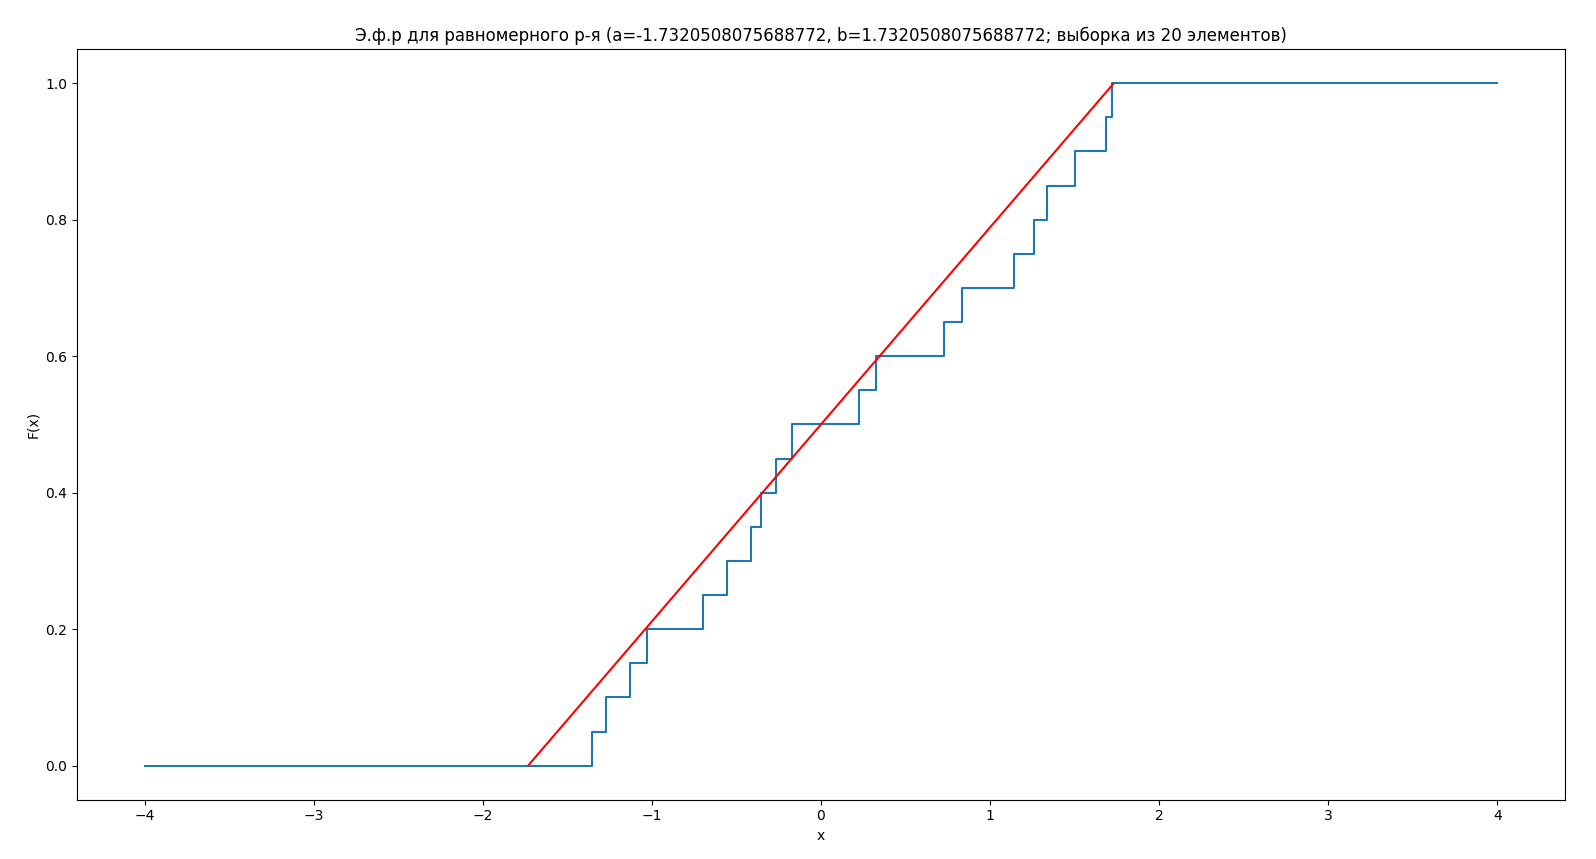
\includegraphics[scale=0.14]{resources/4_uniform_20.png}
		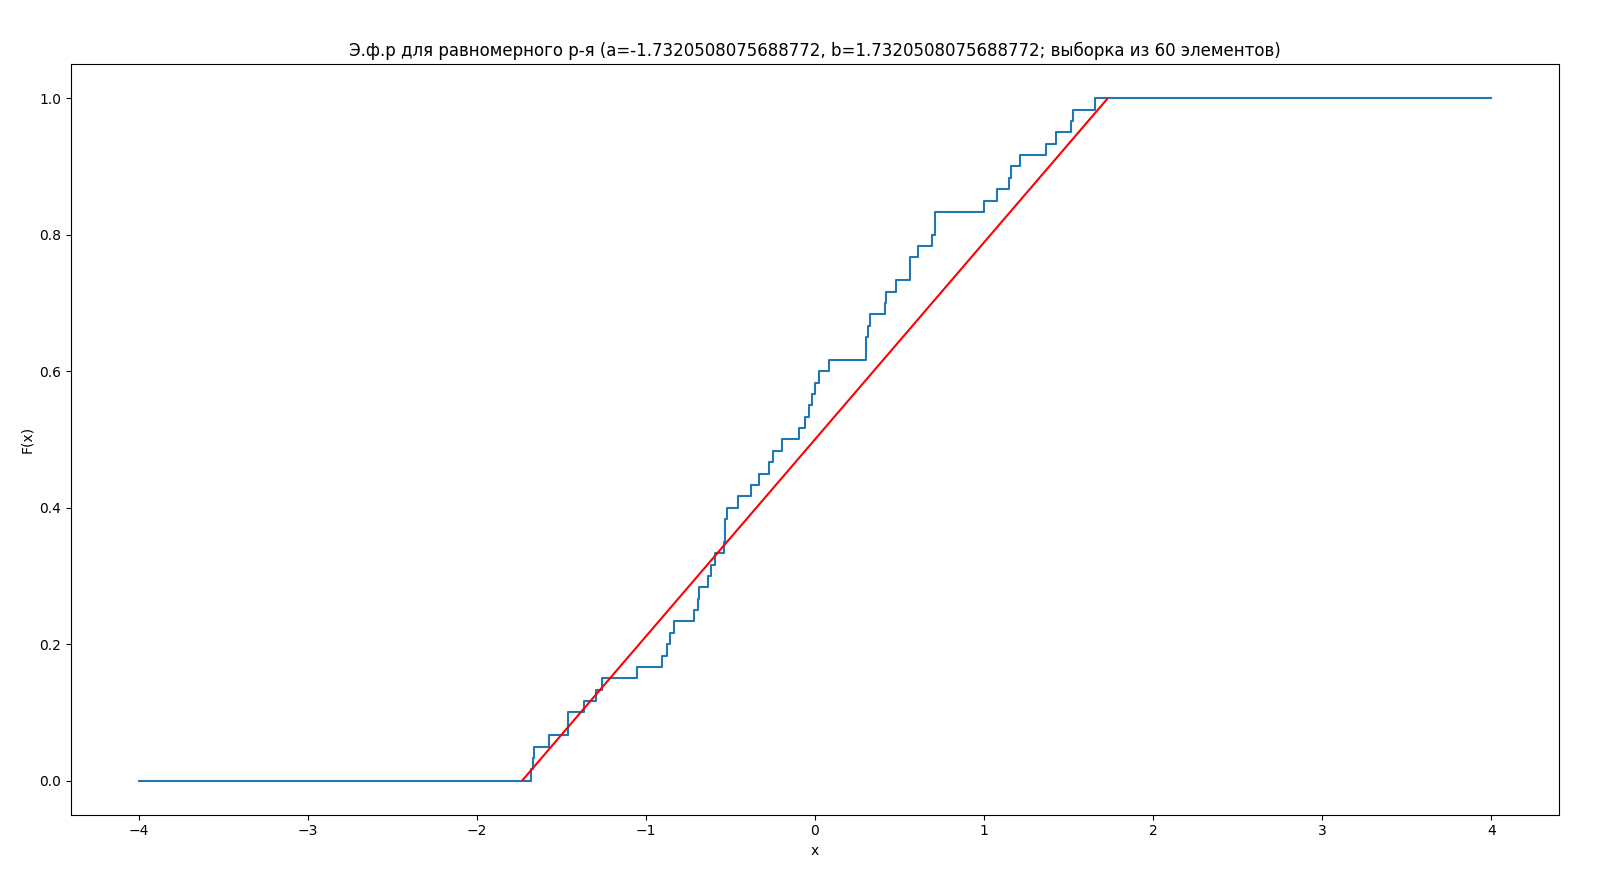
\includegraphics[scale=0.14]{resources/4_uniform_60.png}
		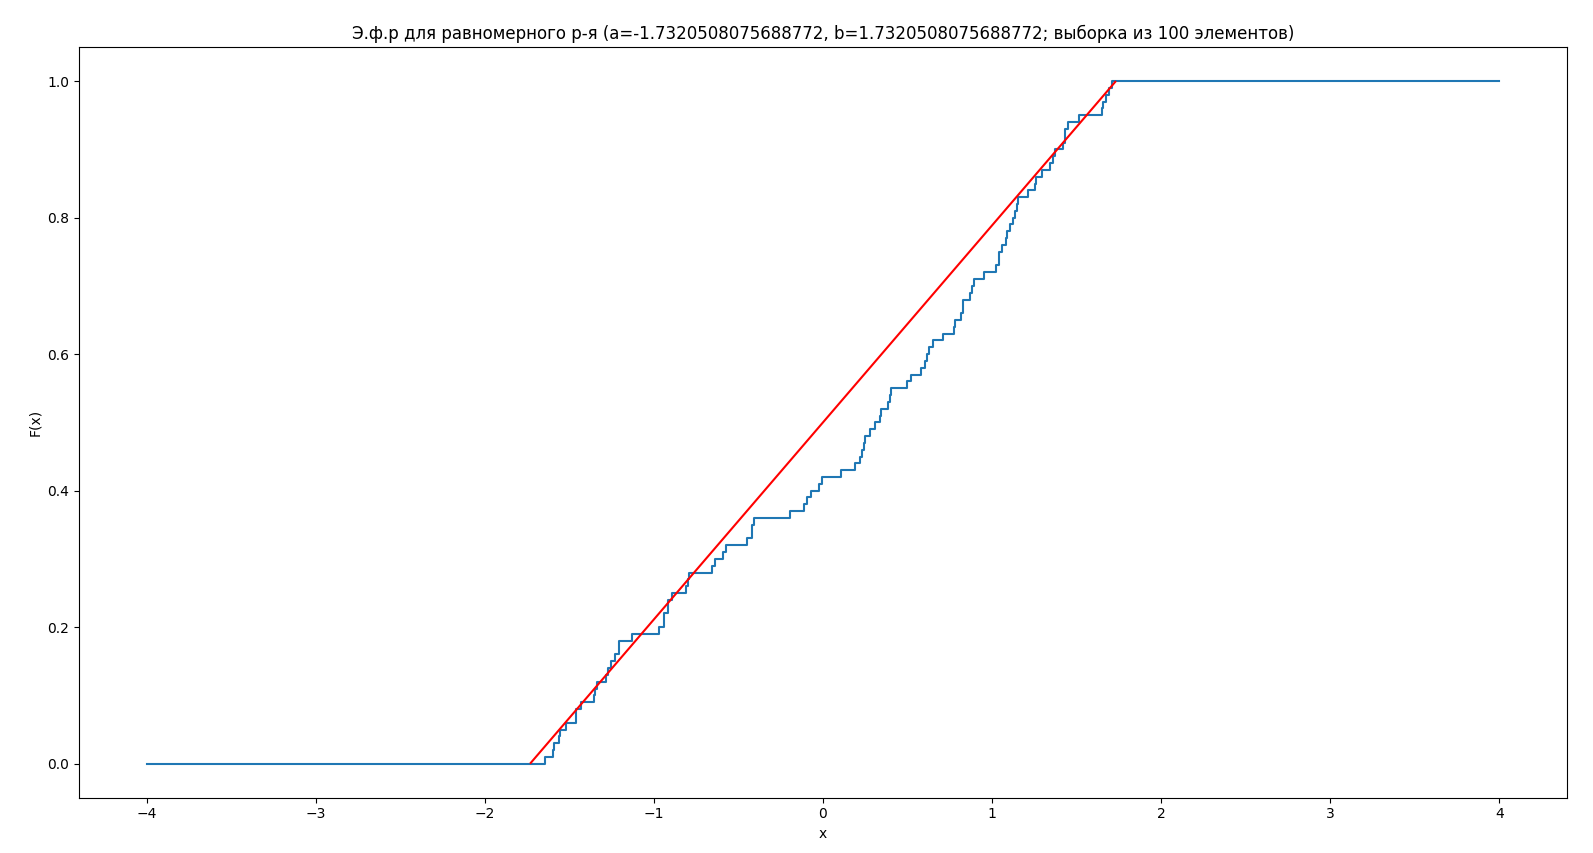
\includegraphics[scale=0.14]{resources/4_uniform_100.png}
	\end{tabular}
	\text{\tab \tab \tab n=20 \tab \tab \tab \tab \tab n=60 \tab \tab \tab \tab \tab n=100 \tab \tab }
	\caption{Равномерное распределение}
\end{figure}

\subsection{Ядерные оценки плотности распределения}

\begin{figure}[H]
	\begin{tabular}{ccc}
		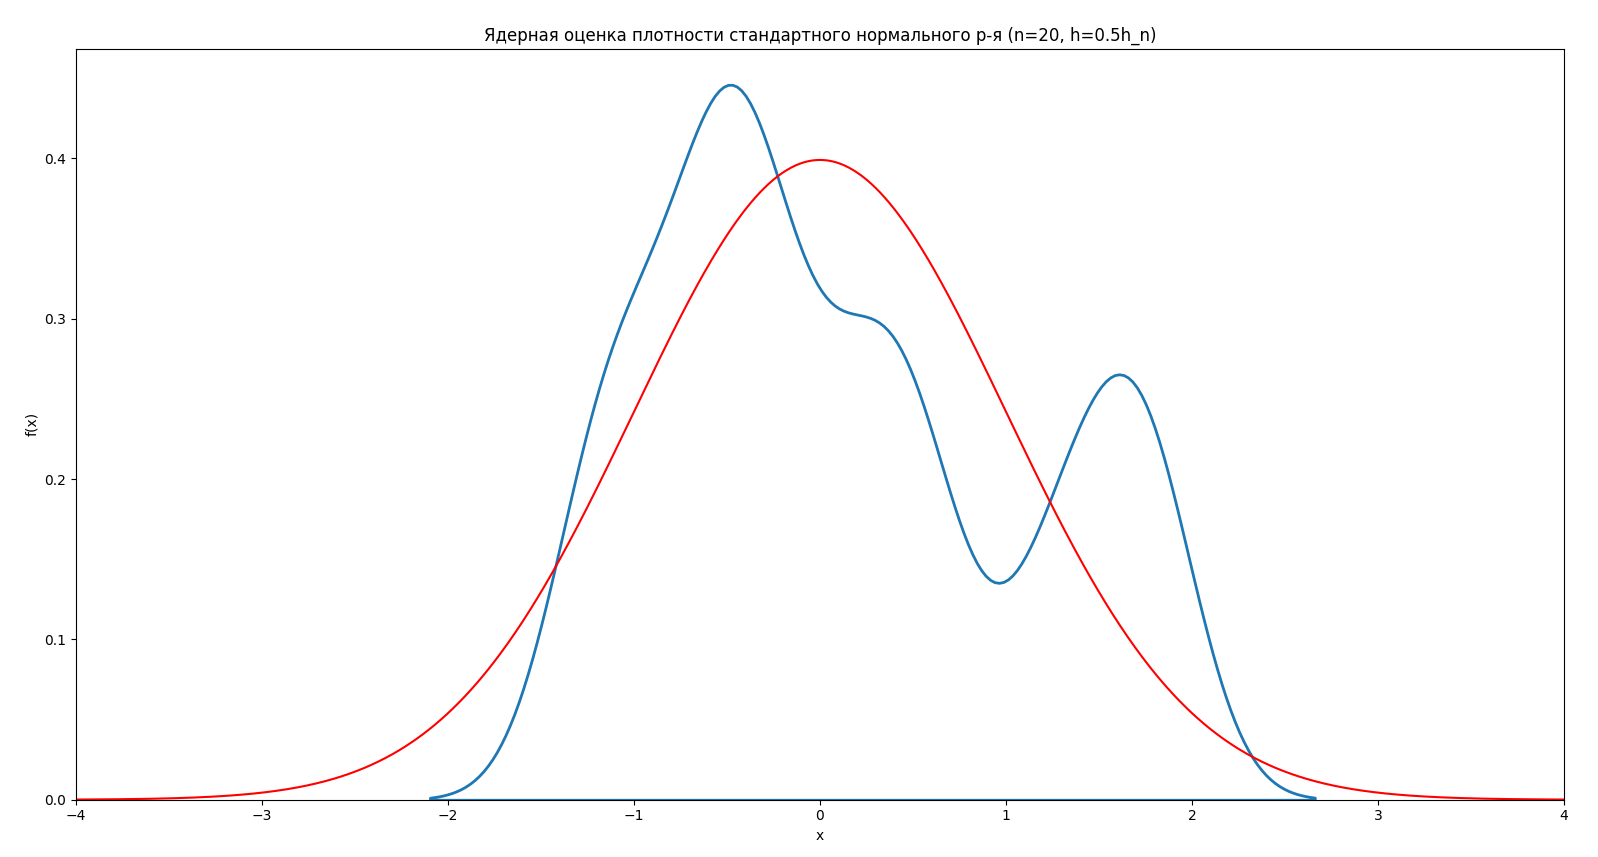
\includegraphics[scale=0.14]{resources/4_gauss_20_half.png}
		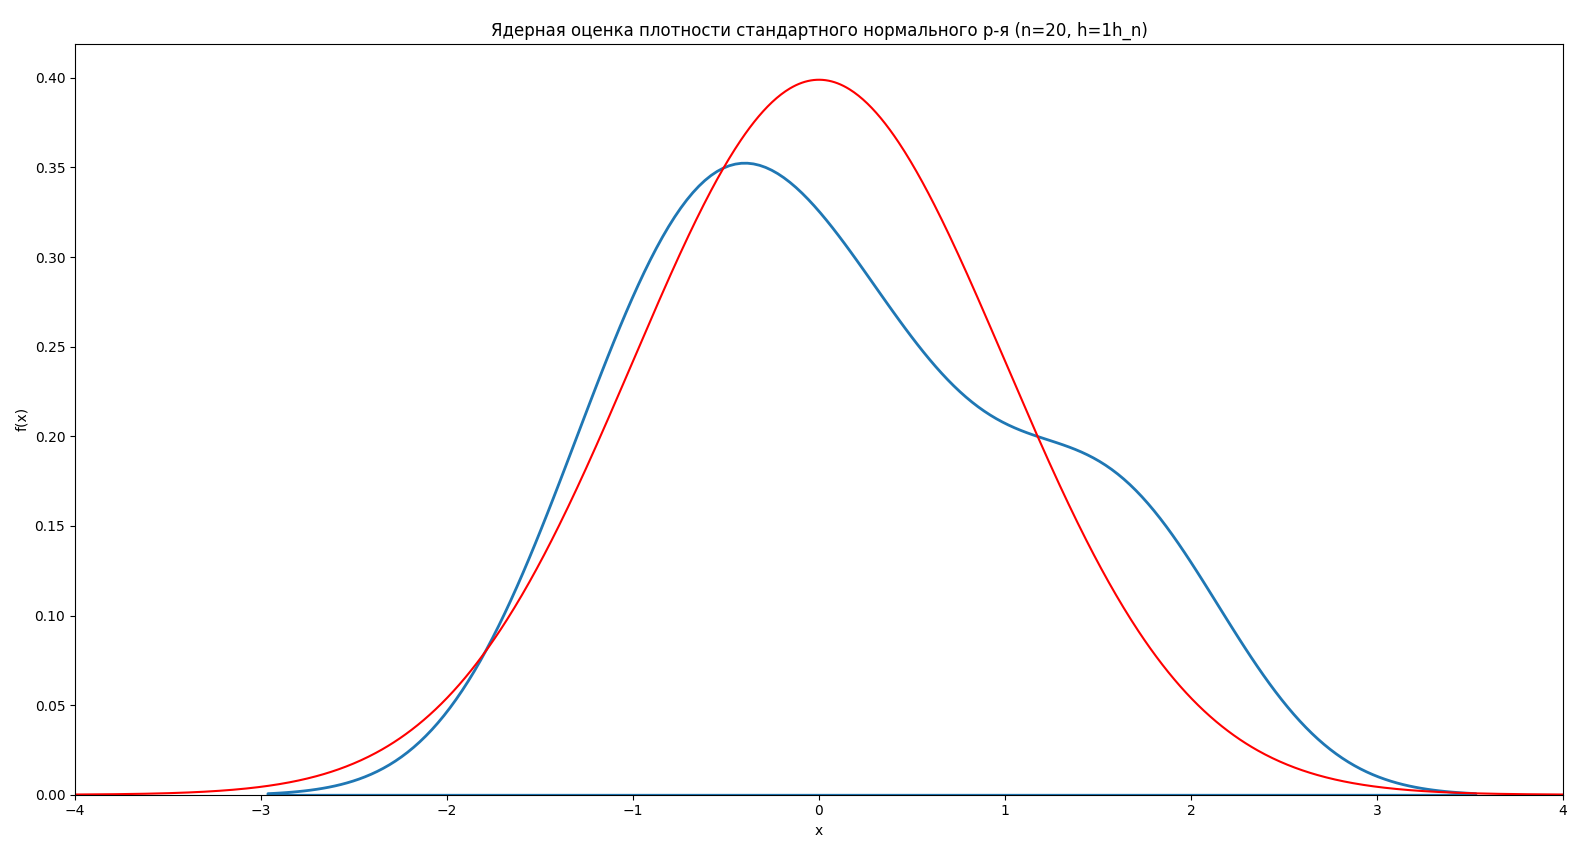
\includegraphics[scale=0.14]{resources/4_gauss_20_one.png}
		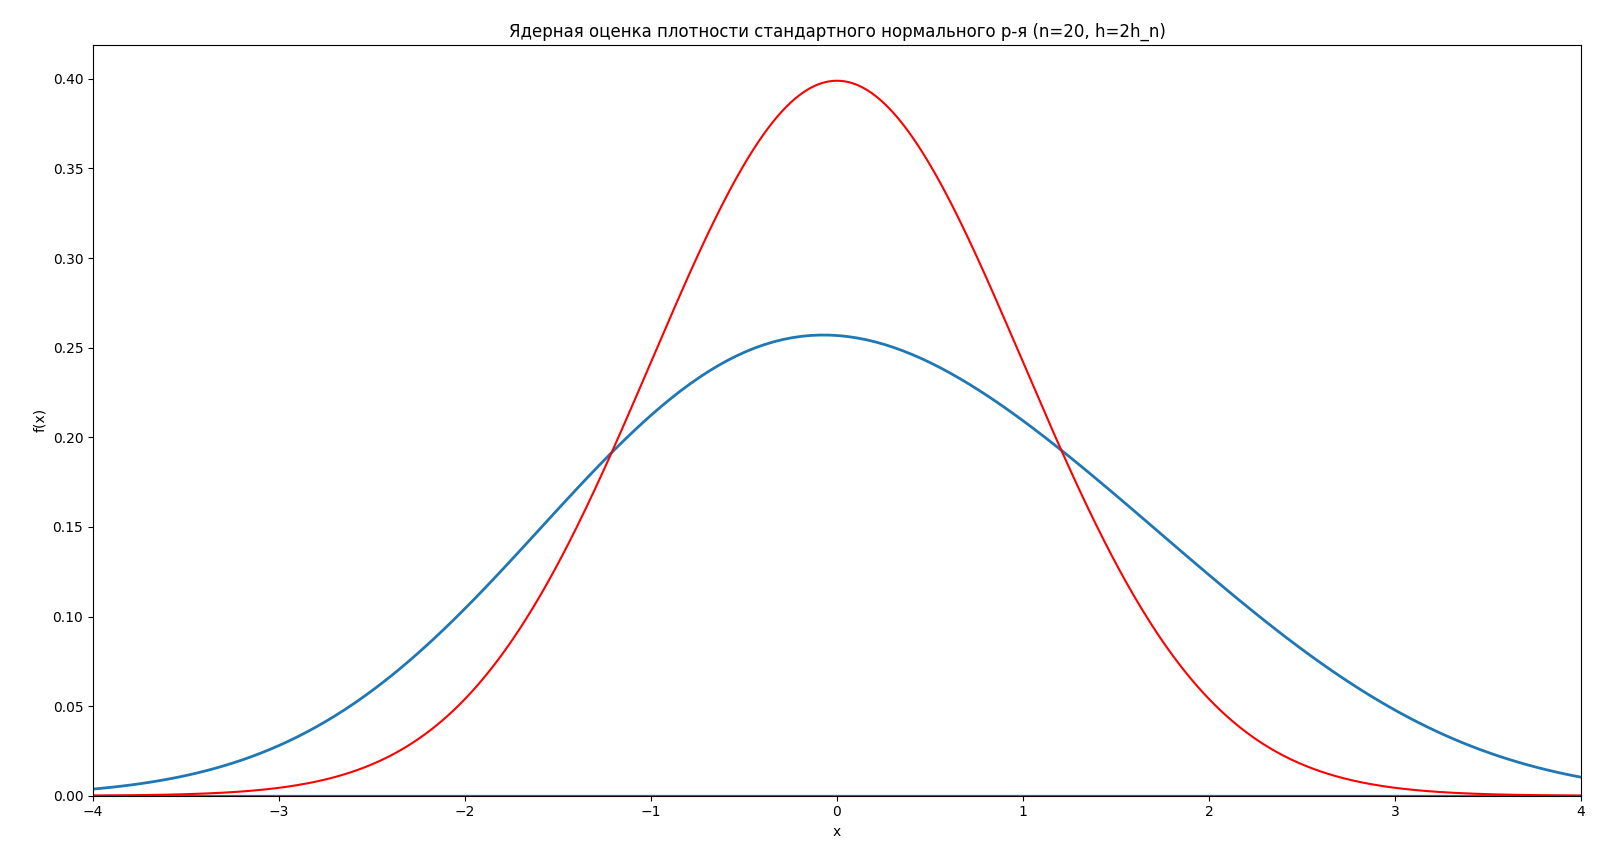
\includegraphics[scale=0.14]{resources/4_gauss_20_two.png}
	\end{tabular}
	\text{\tab \tab $h=h_{n}/2$ \tab \tab \tab \tab \tab $h=h_{n}$ \tab \tab \tab \tab \tab $h=2h_{n}$ \tab \tab }
	\caption{Нормальное распределение, $n=20$}
\end{figure}

\begin{figure}[H]
	\begin{tabular}{ccc}
		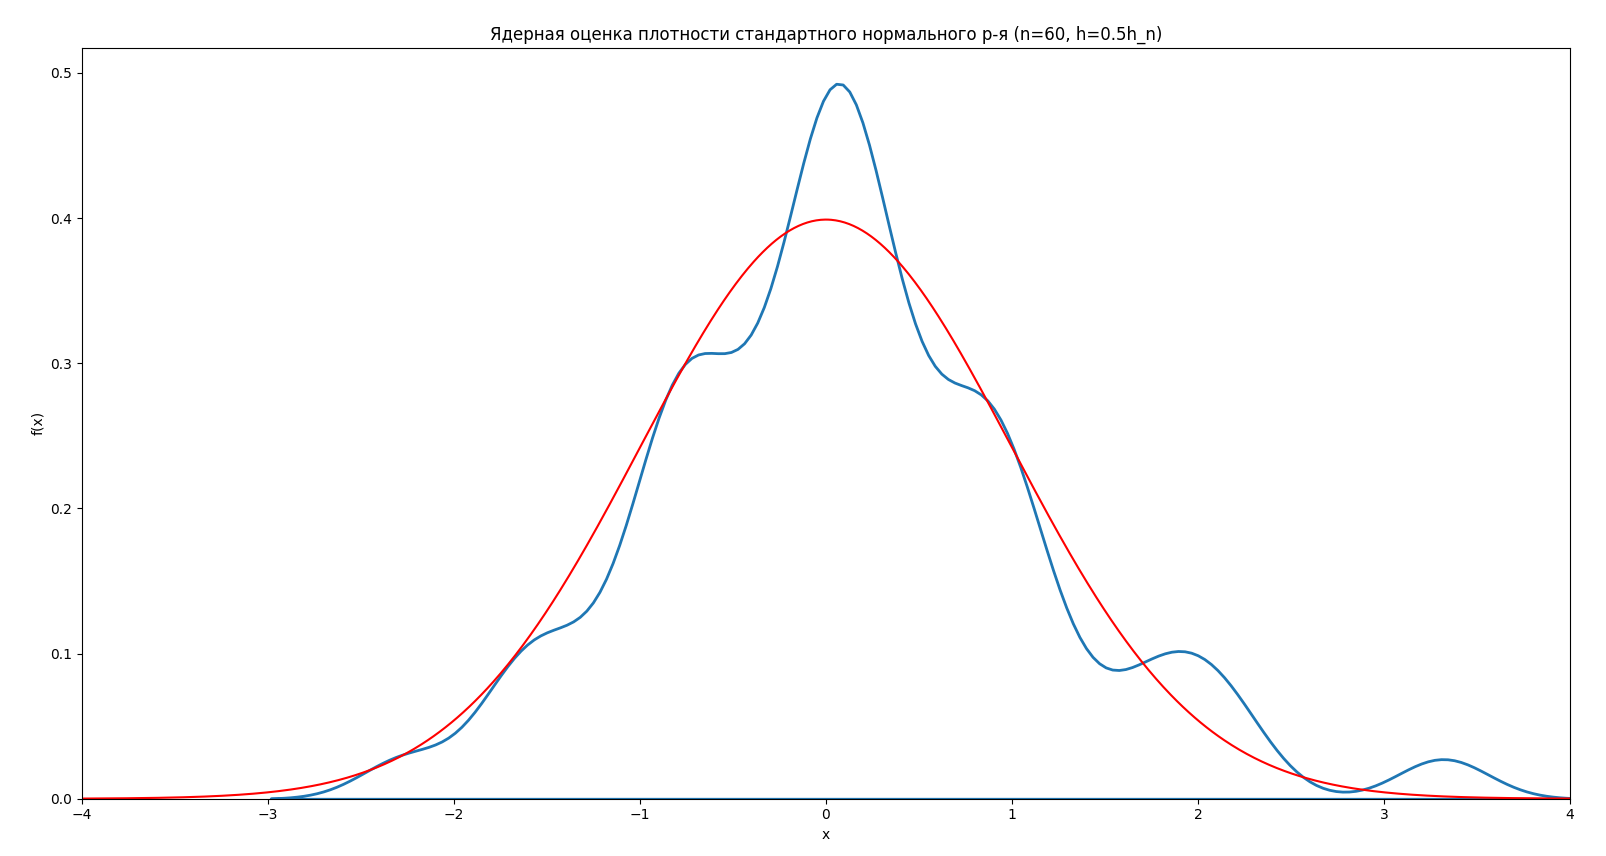
\includegraphics[scale=0.14]{resources/4_gauss_60_half.png}
		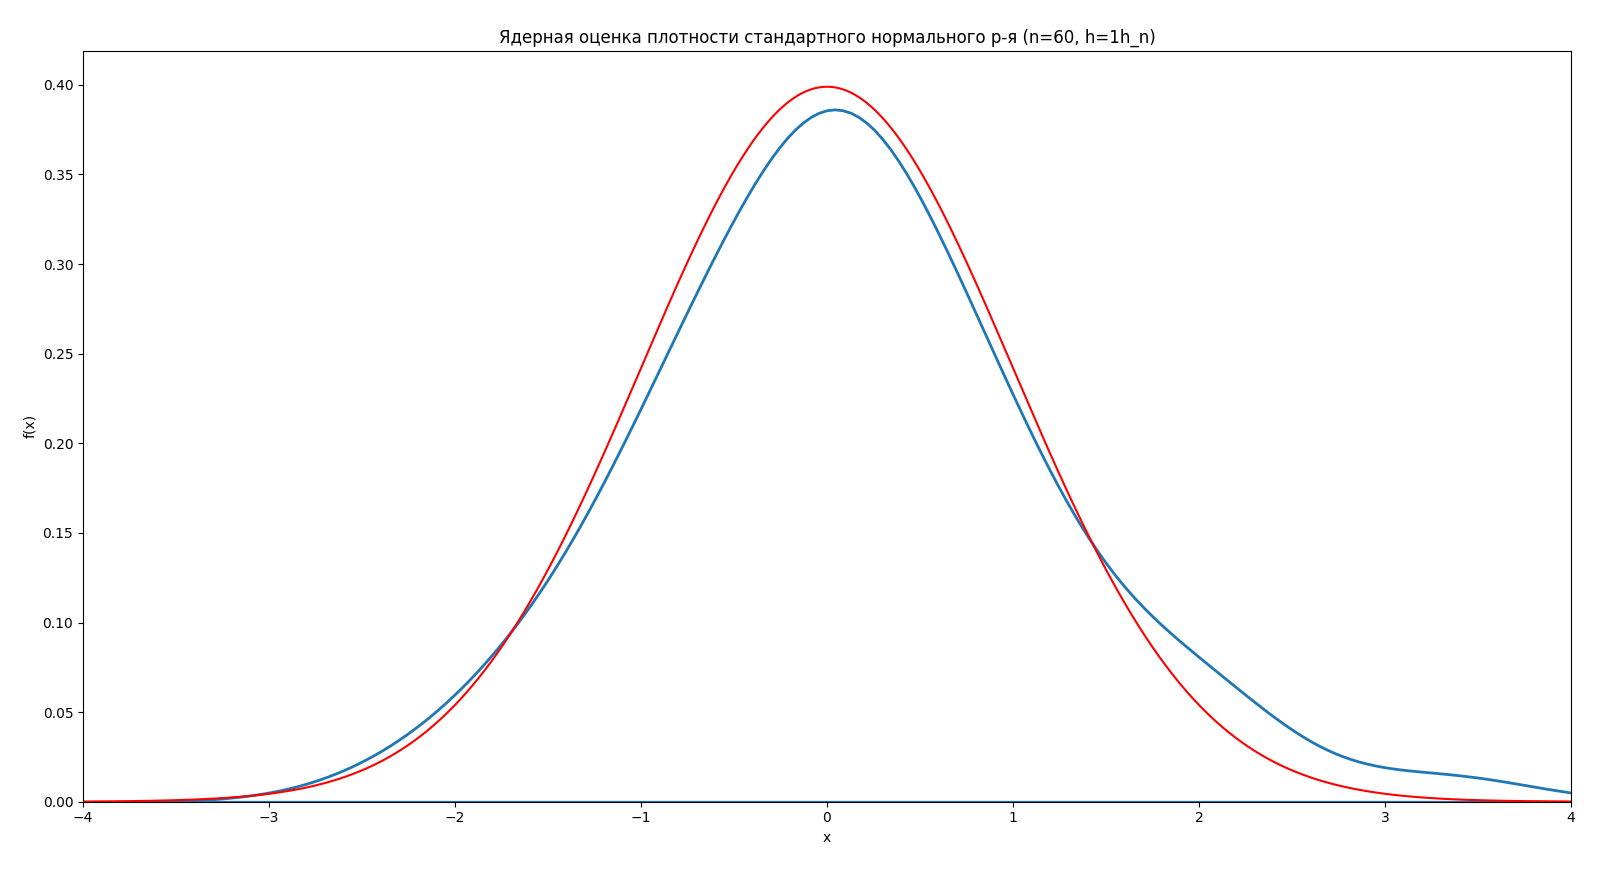
\includegraphics[scale=0.14]{resources/4_gauss_60_one.png}
		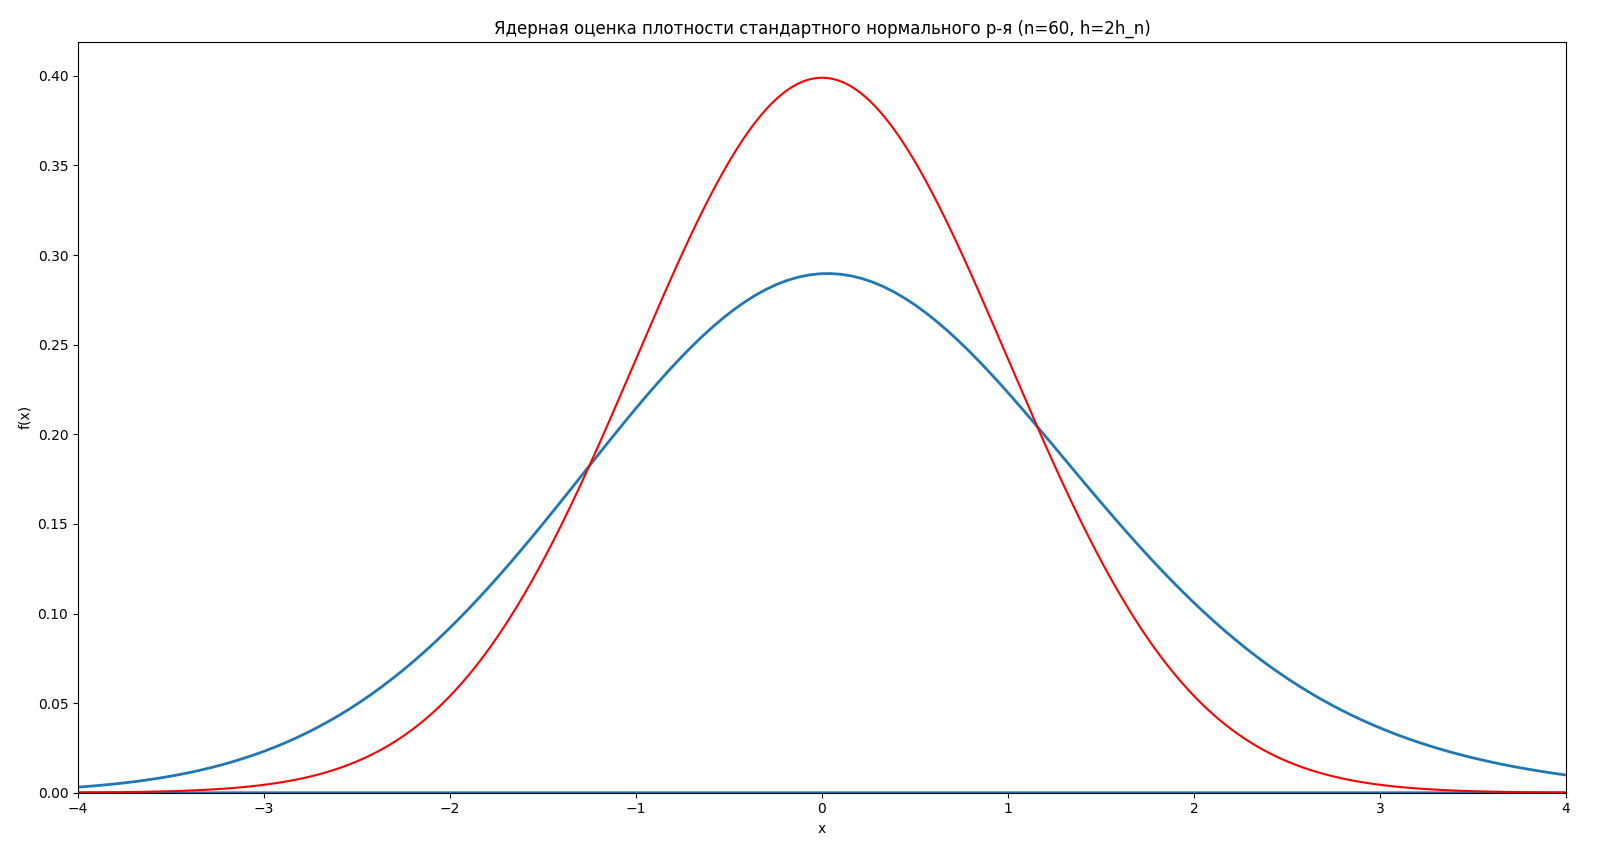
\includegraphics[scale=0.14]{resources/4_gauss_60_two.png}
	\end{tabular}
	\text{\tab \tab $h=h_{n}/2$ \tab \tab \tab \tab \tab $h=h_{n}$ \tab \tab \tab \tab \tab $h=2h_{n}$ \tab \tab }
	\caption{Нормальное распределение, $n=60$}
\end{figure}

\begin{figure}[H]
	\begin{tabular}{ccc}
		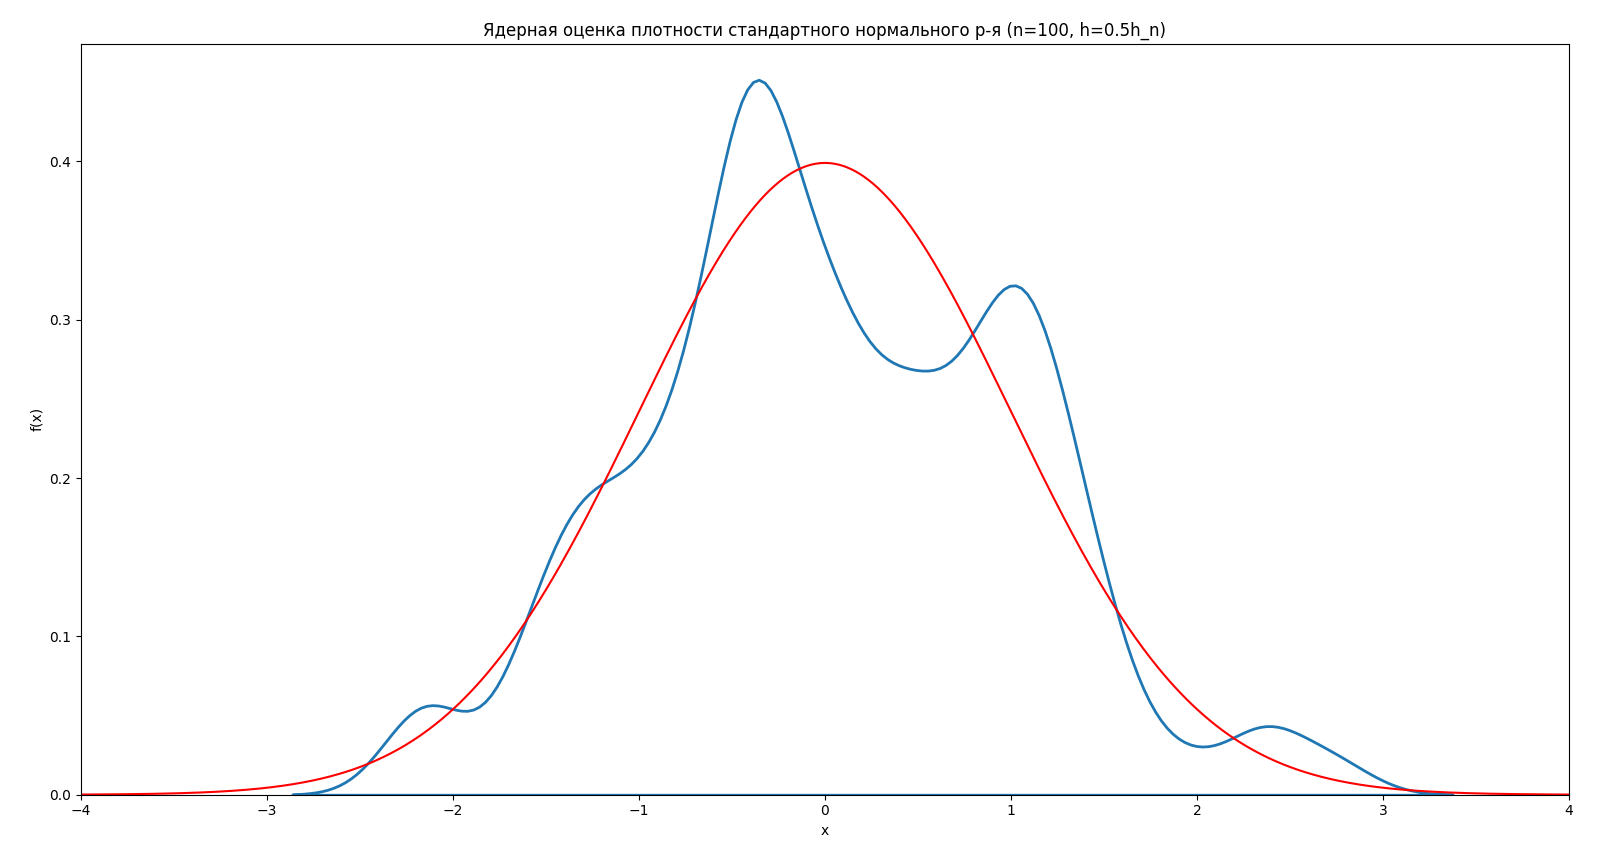
\includegraphics[scale=0.14]{resources/4_gauss_100_half.png}
		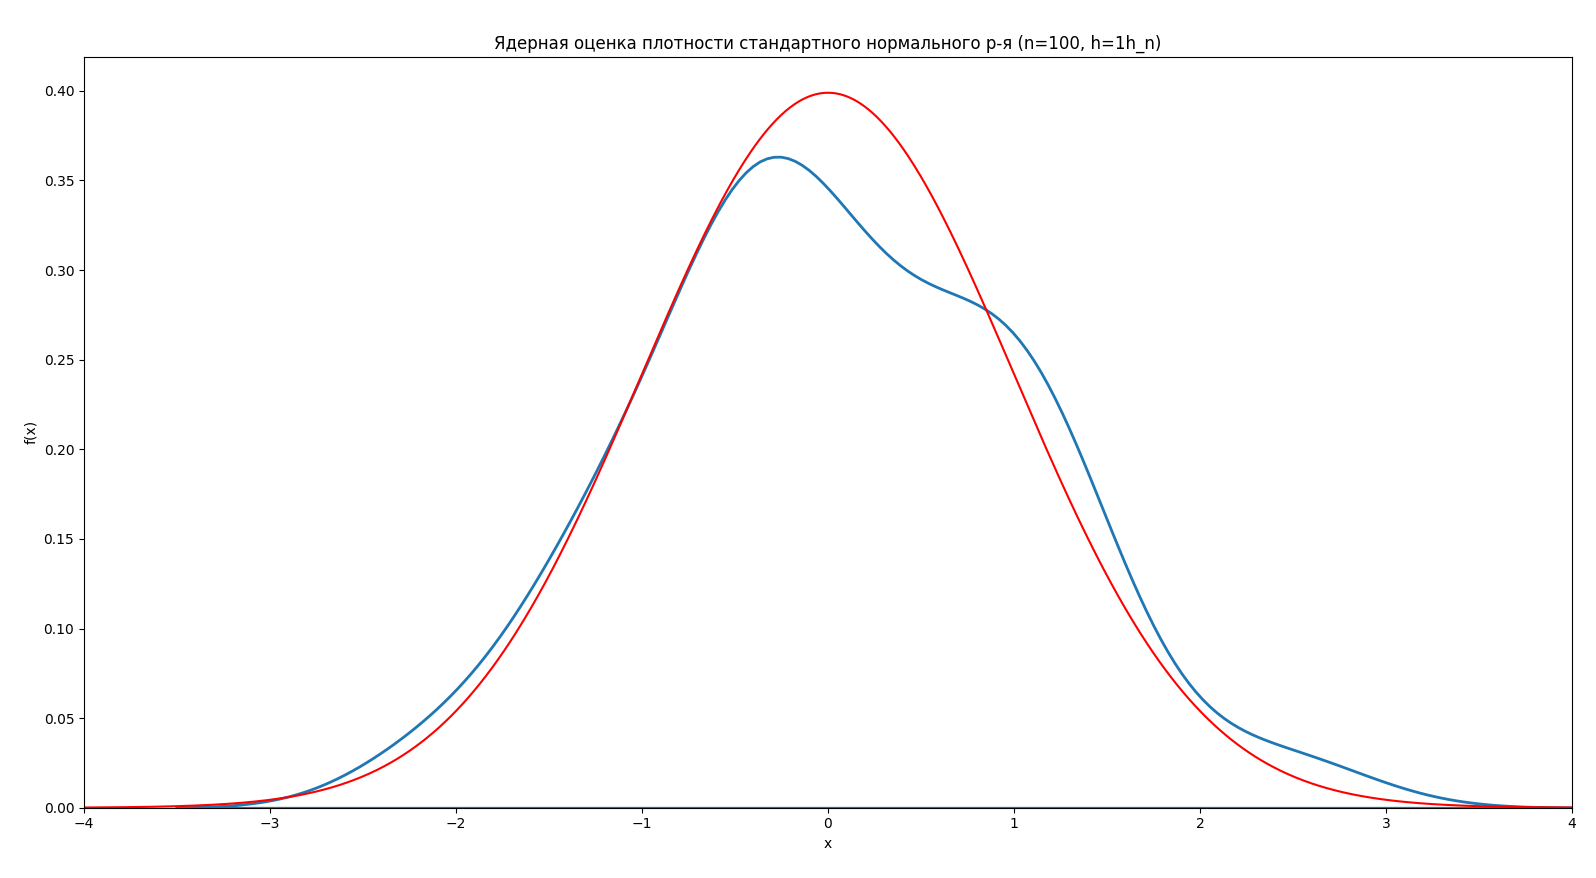
\includegraphics[scale=0.14]{resources/4_gauss_100_one.png}
		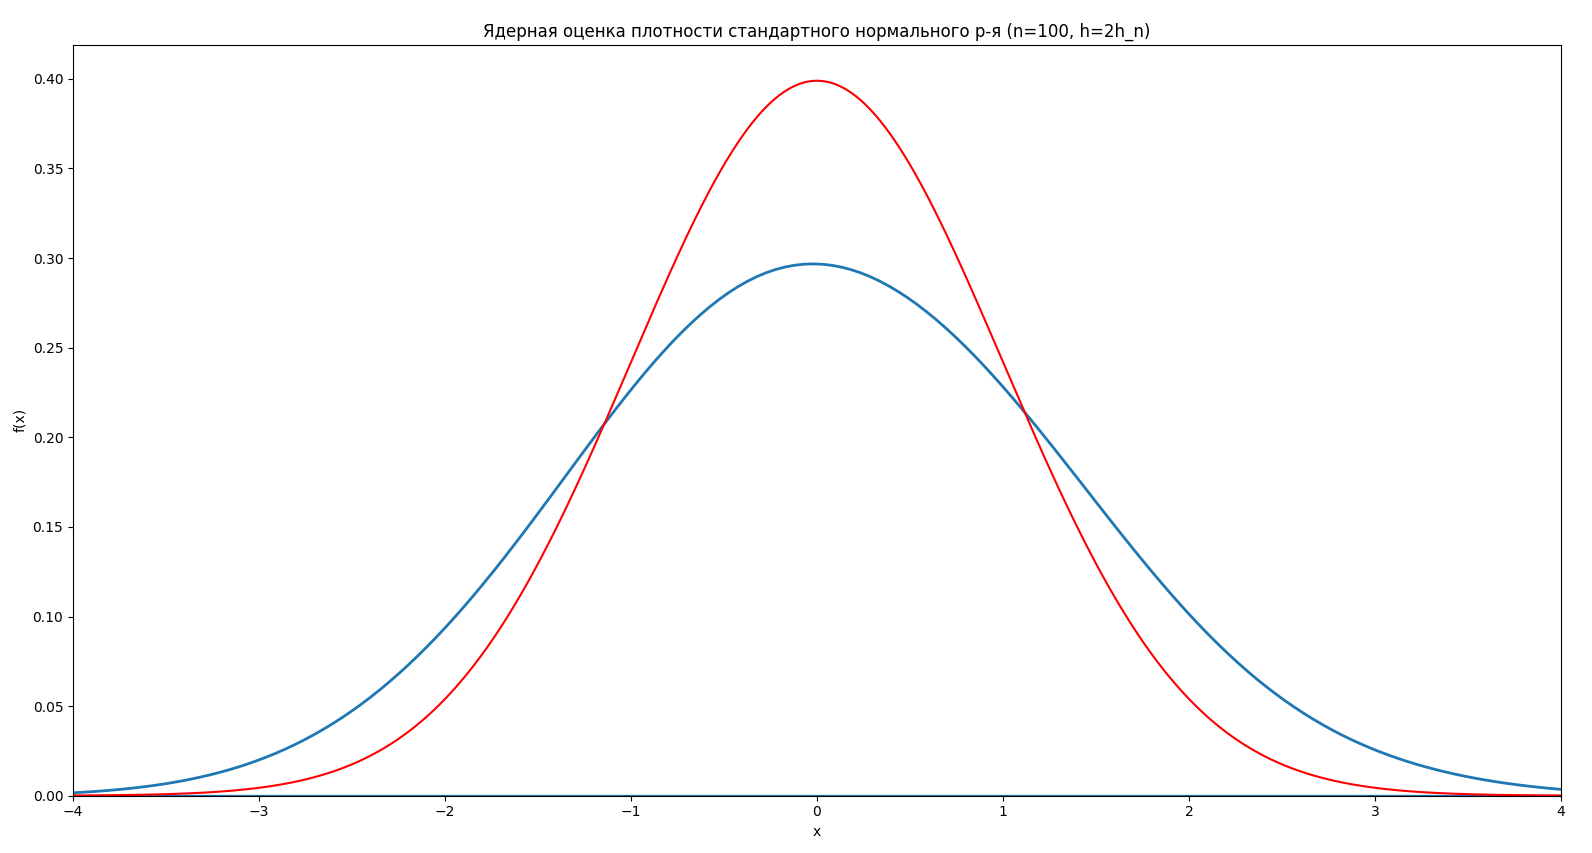
\includegraphics[scale=0.14]{resources/4_gauss_100_two.png}
	\end{tabular}
	\text{\tab \tab $h=h_{n}/2$ \tab \tab \tab \tab \tab $h=h_{n}$ \tab \tab \tab \tab \tab $h=2h_{n}$ \tab \tab }
	\caption{Нормальное распределение, $n=100$}
\end{figure}

\begin{figure}[H]
	\begin{tabular}{ccc}
		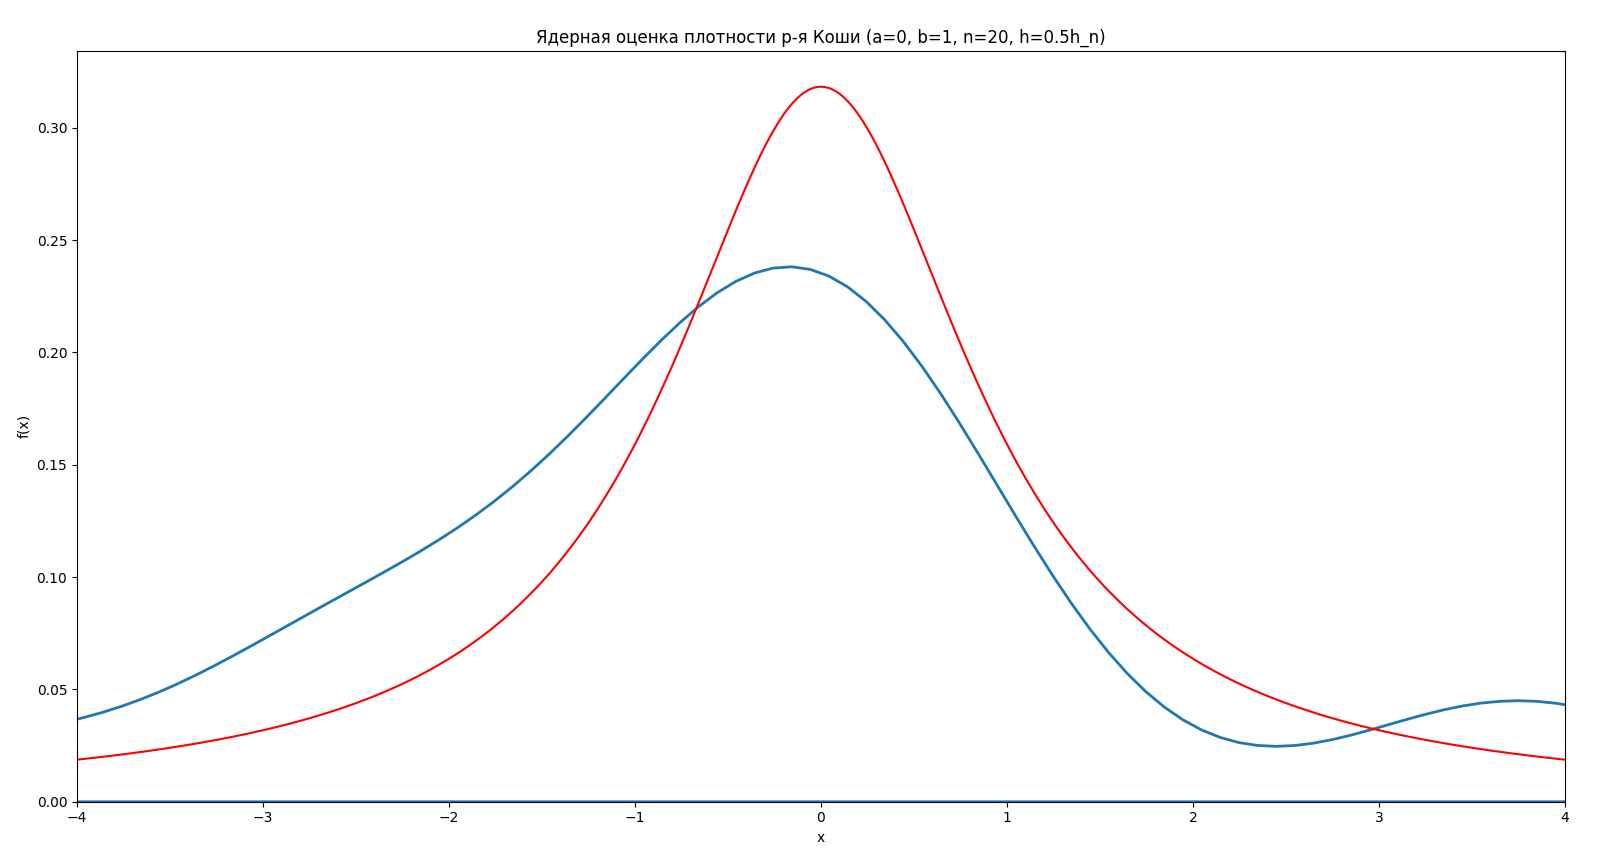
\includegraphics[scale=0.14]{resources/4_cauchy_20_half.png}
		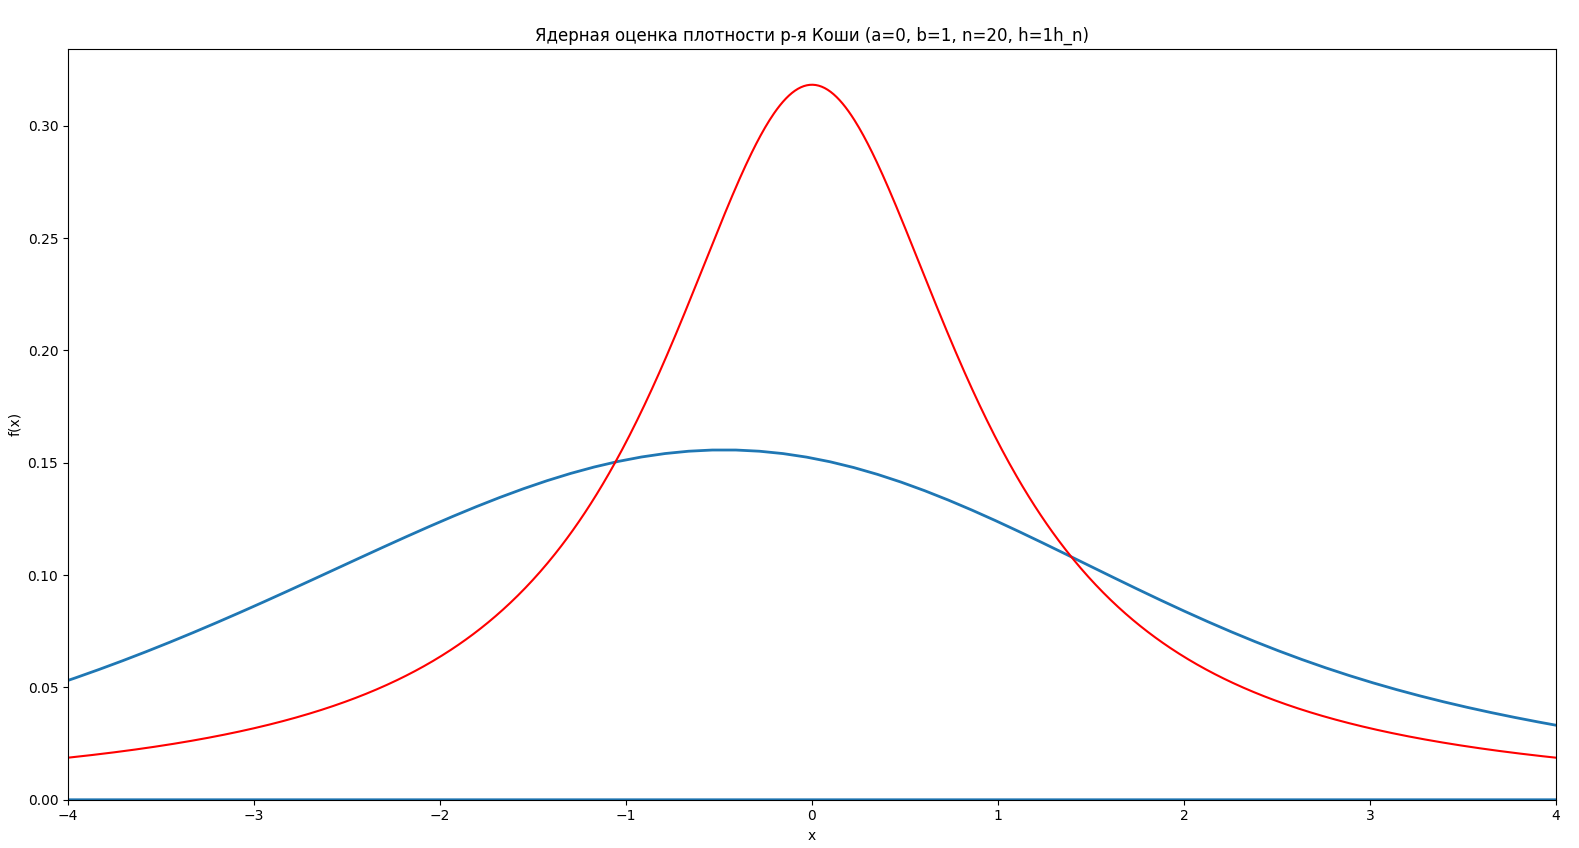
\includegraphics[scale=0.14]{resources/4_cauchy_20_one.png}
		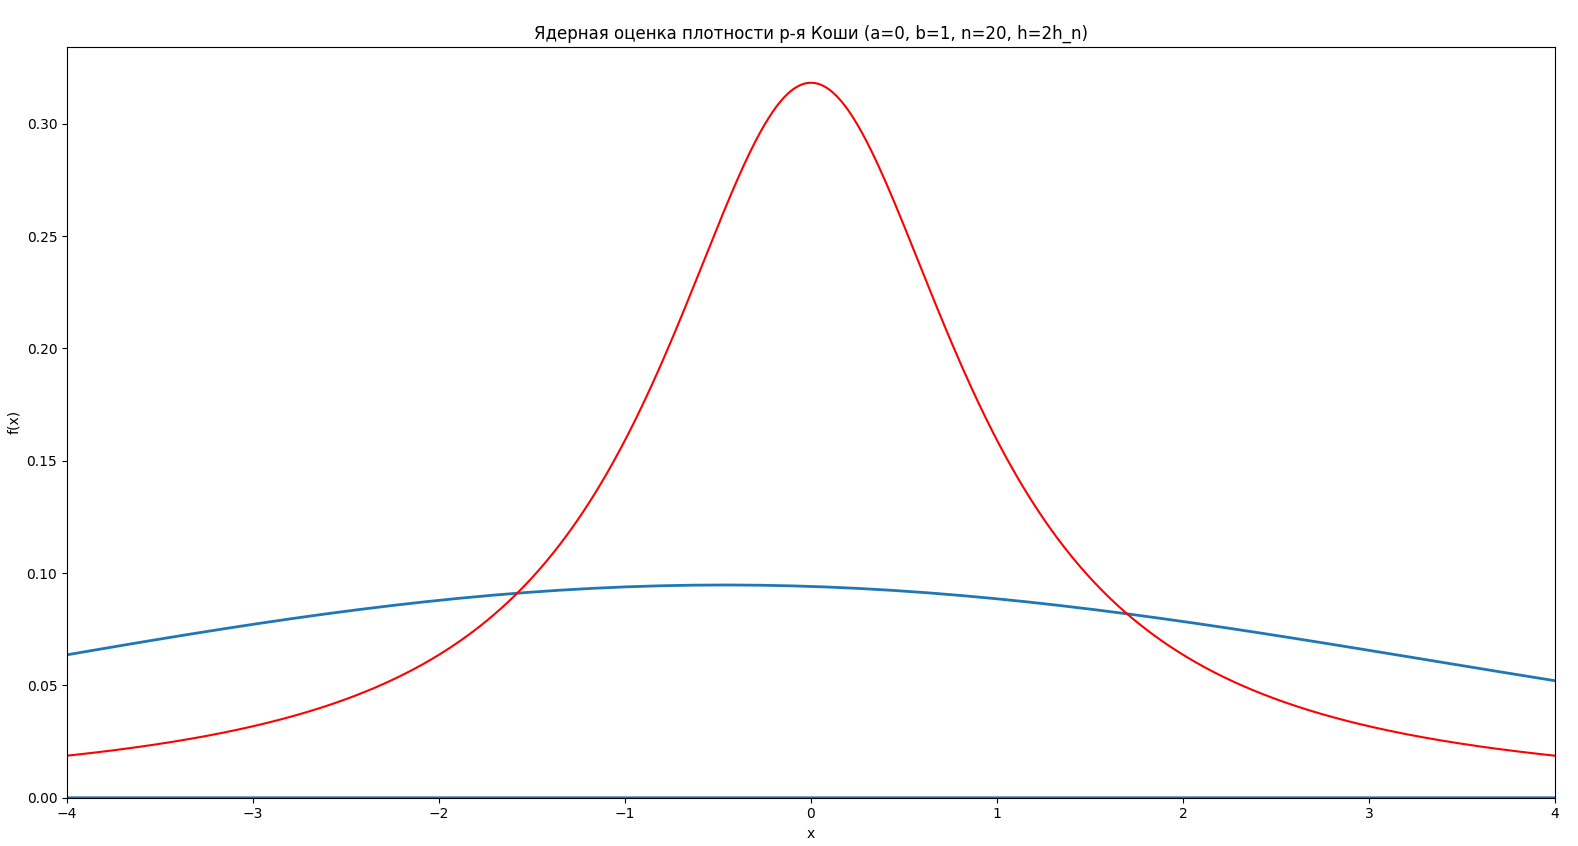
\includegraphics[scale=0.14]{resources/4_cauchy_20_two.png}
	\end{tabular}
	\text{\tab \tab $h=h_{n}/2$ \tab \tab \tab \tab \tab $h=h_{n}$ \tab \tab \tab \tab \tab $h=2h_{n}$ \tab \tab }
	\caption{Распределение Коши, $n=20$}
\end{figure}

\begin{figure}[H]
	\begin{tabular}{ccc}
		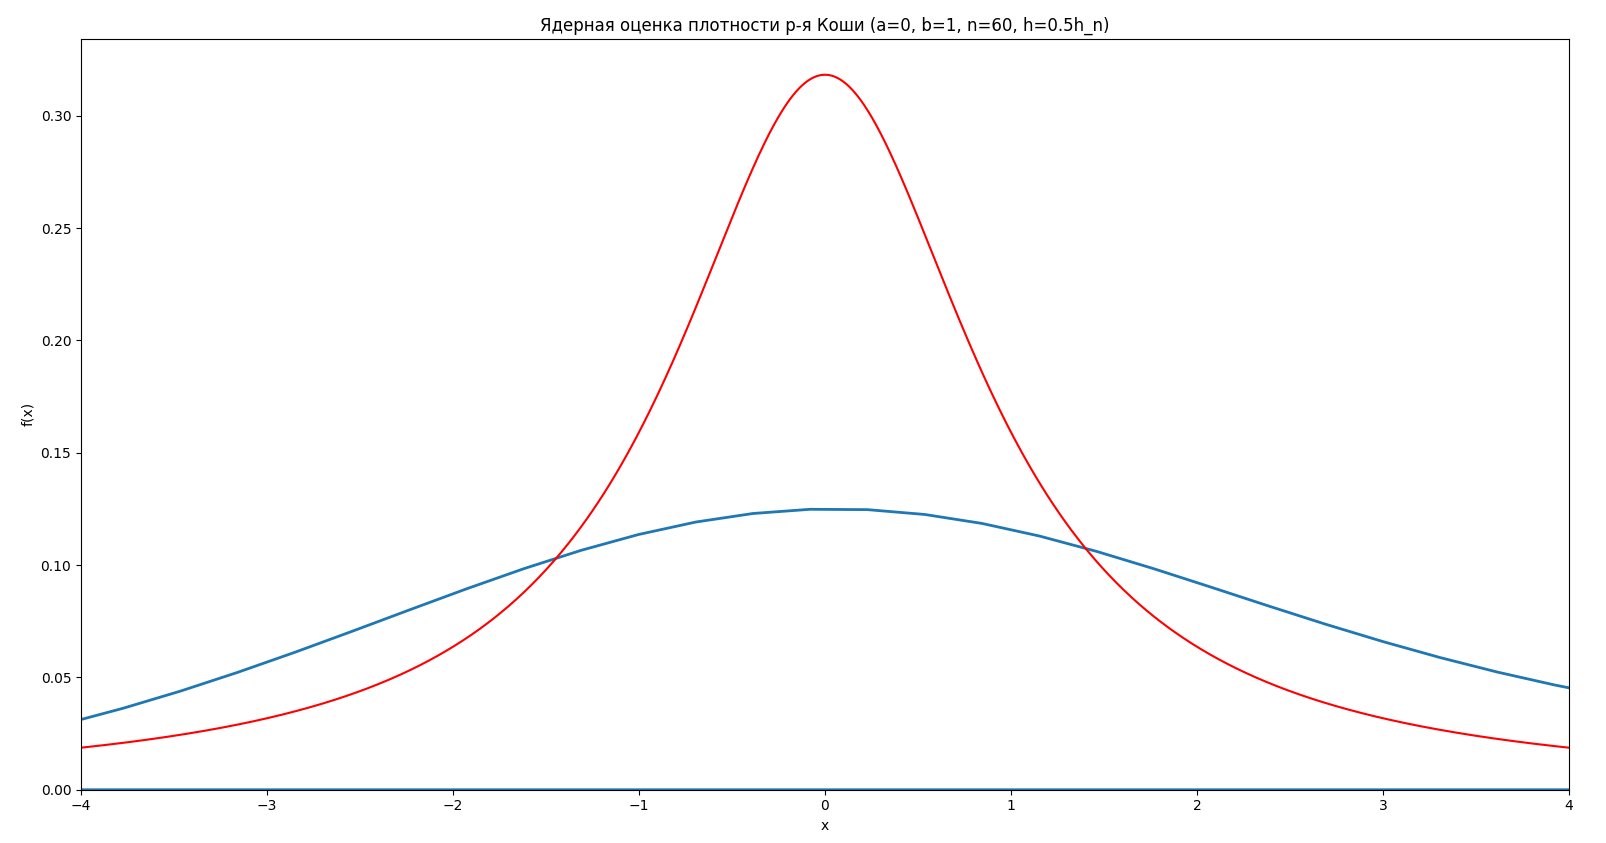
\includegraphics[scale=0.14]{resources/4_cauchy_60_half.png}
		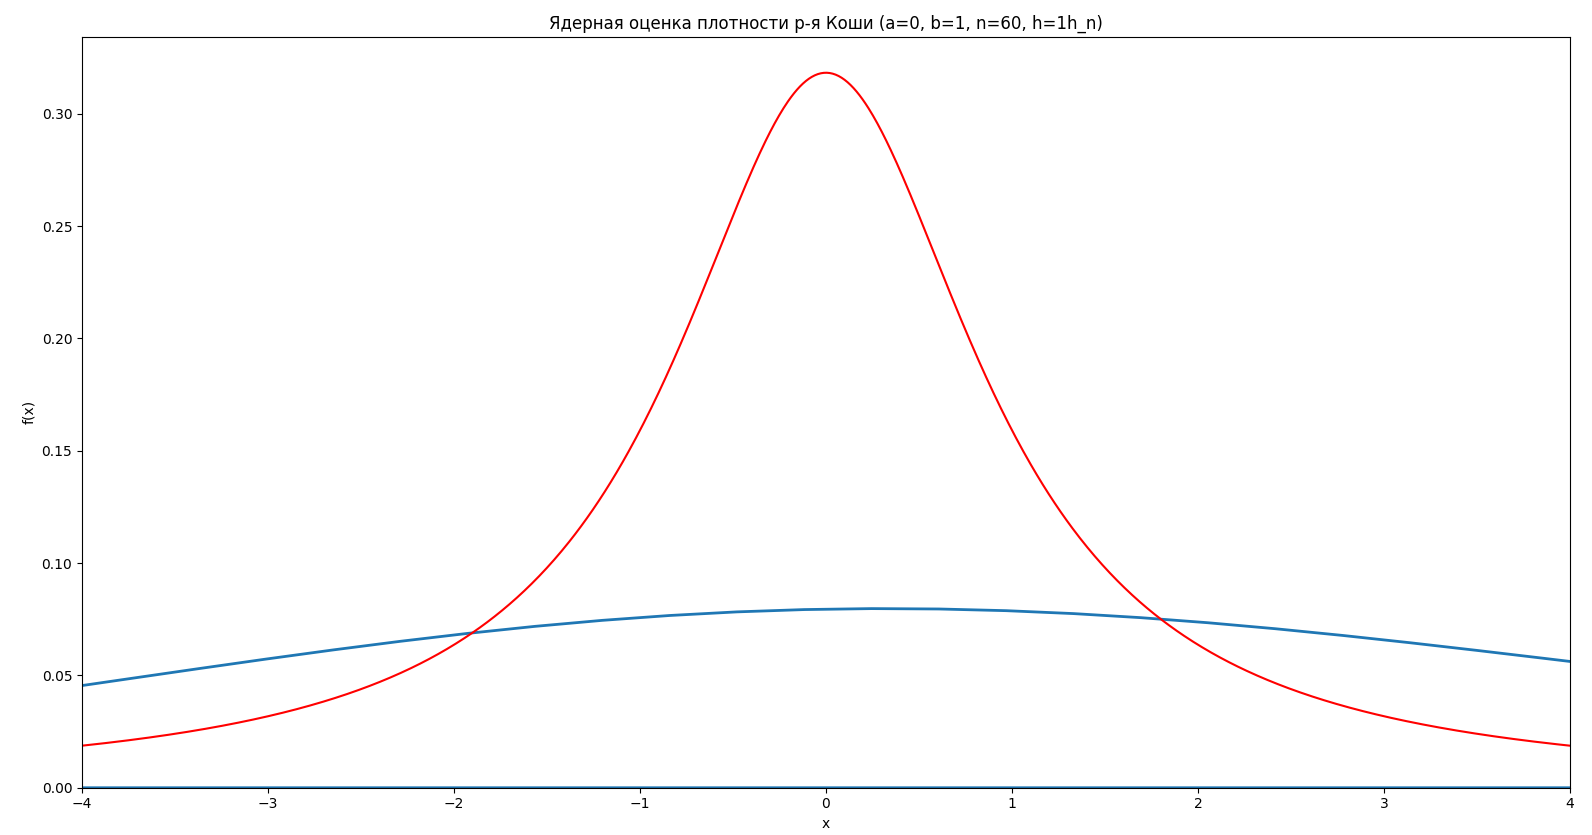
\includegraphics[scale=0.14]{resources/4_cauchy_60_one.png}
		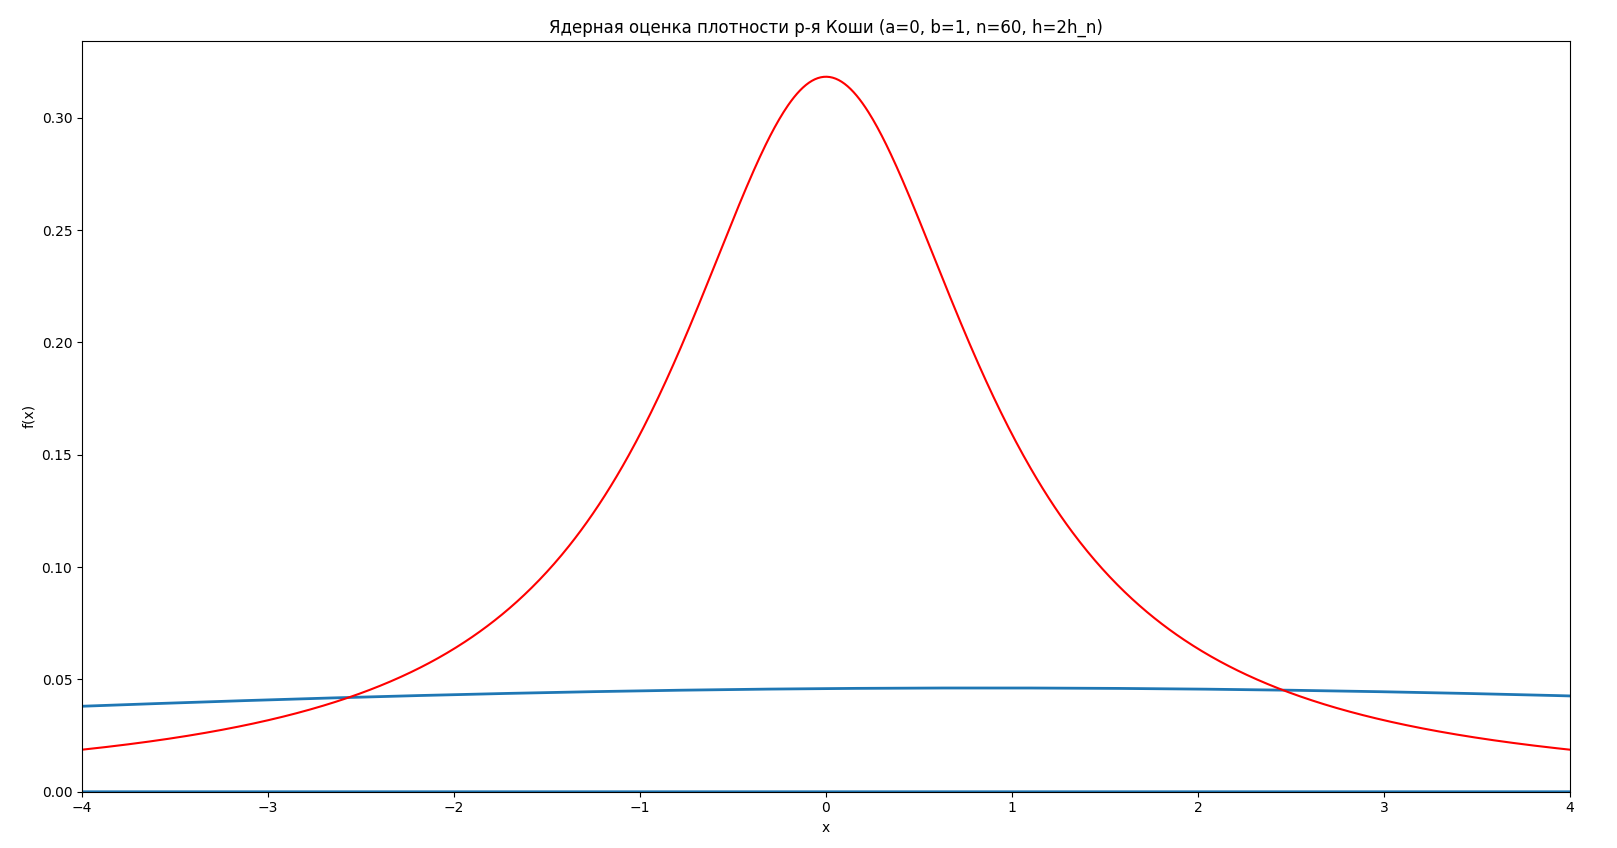
\includegraphics[scale=0.14]{resources/4_cauchy_60_two.png}
	\end{tabular}
	\text{\tab \tab $h=h_{n}/2$ \tab \tab \tab \tab \tab $h=h_{n}$ \tab \tab \tab \tab \tab $h=2h_{n}$ \tab \tab }
	\caption{Распределение Коши, $n=60$}
\end{figure}

\begin{figure}[H]
	\begin{tabular}{ccc}
		\includegraphics[scale=0.14]{resources/4_cauchy_100_half.png}
		\includegraphics[scale=0.14]{resources/4_cauchy_100_one.png}
		\includegraphics[scale=0.14]{resources/4_cauchy_100_two.png}
	\end{tabular}
	\text{\tab \tab $h=h_{n}/2$ \tab \tab \tab \tab \tab $h=h_{n}$ \tab \tab \tab \tab \tab $h=2h_{n}$ \tab \tab }
	\caption{Распределение Коши, $n=100$}
\end{figure}

\begin{figure}[H]
	\begin{tabular}{ccc}
		\includegraphics[scale=0.14]{resources/4_laplace_20_half.png}
		\includegraphics[scale=0.14]{resources/4_laplace_20_one.png}
		\includegraphics[scale=0.14]{resources/4_laplace_20_two.png}
	\end{tabular}
	\text{\tab \tab $h=h_{n}/2$ \tab \tab \tab \tab \tab $h=h_{n}$ \tab \tab \tab \tab \tab $h=2h_{n}$ \tab \tab }
	\caption{Распределение Лапласа, $n=20$}
\end{figure}

\begin{figure}[H]
	\begin{tabular}{ccc}
		\includegraphics[scale=0.14]{resources/4_laplace_60_half.png}
		\includegraphics[scale=0.14]{resources/4_laplace_60_one.png}
		\includegraphics[scale=0.14]{resources/4_laplace_60_two.png}
	\end{tabular}
	\text{\tab \tab $h=h_{n}/2$ \tab \tab \tab \tab \tab $h=h_{n}$ \tab \tab \tab \tab \tab $h=2h_{n}$ \tab \tab }
	\caption{Распределение Лапласа, $n=60$}
\end{figure}

\begin{figure}[H]
	\begin{tabular}{ccc}
		\includegraphics[scale=0.14]{resources/4_laplace_100_half.png}
		\includegraphics[scale=0.14]{resources/4_laplace_100_one.png}
		\includegraphics[scale=0.14]{resources/4_laplace_100_two.png}
	\end{tabular}
	\text{\tab \tab $h=h_{n}/2$ \tab \tab \tab \tab \tab $h=h_{n}$ \tab \tab \tab \tab \tab $h=2h_{n}$ \tab \tab }
	\caption{Распределение Лапласа, $n=100$}
\end{figure}

\begin{figure}[H]
	\begin{tabular}{ccc}
		\includegraphics[scale=0.14]{resources/4_poisson_20_half.png}
		\includegraphics[scale=0.14]{resources/4_poisson_20_one.png}
		\includegraphics[scale=0.14]{resources/4_poisson_20_two.png}
	\end{tabular}
	\text{\tab \tab $h=h_{n}/2$ \tab \tab \tab \tab \tab $h=h_{n}$ \tab \tab \tab \tab \tab $h=2h_{n}$ \tab \tab }
	\caption{Распределение Пуассона, $n=20$}
\end{figure}

\begin{figure}[H]
	\begin{tabular}{ccc}
		\includegraphics[scale=0.14]{resources/4_poisson_60_half.png}
		\includegraphics[scale=0.14]{resources/4_poisson_60_one.png}
		\includegraphics[scale=0.14]{resources/4_poisson_60_two.png}
	\end{tabular}
	\text{\tab \tab $h=h_{n}/2$ \tab \tab \tab \tab \tab $h=h_{n}$ \tab \tab \tab \tab \tab $h=2h_{n}$ \tab \tab }
	\caption{Распределение Пуассона, $n=60$}
\end{figure}

\begin{figure}[H]
	\begin{tabular}{ccc}
		\includegraphics[scale=0.14]{resources/4_poisson_100_half.png}
		\includegraphics[scale=0.14]{resources/4_poisson_100_one.png}
		\includegraphics[scale=0.14]{resources/4_poisson_100_two.png}
	\end{tabular}
	\text{\tab \tab $h=h_{n}/2$ \tab \tab \tab \tab \tab $h=h_{n}$ \tab \tab \tab \tab \tab $h=2h_{n}$ \tab \tab }
	\caption{Распределение Пуассона, $n=100$}
\end{figure}

\begin{figure}[H]
	\begin{tabular}{ccc}
		\includegraphics[scale=0.14]{resources/4_uniform_20_half.png}
		\includegraphics[scale=0.14]{resources/4_uniform_20_one.png}
		\includegraphics[scale=0.14]{resources/4_uniform_20_two.png}
	\end{tabular}
	\text{\tab \tab $h=h_{n}/2$ \tab \tab \tab \tab \tab $h=h_{n}$ \tab \tab \tab \tab \tab $h=2h_{n}$ \tab \tab }
	\caption{Равномерное распределение, $n=20$}
\end{figure}

\begin{figure}[H]
	\begin{tabular}{ccc}
		\includegraphics[scale=0.14]{resources/4_uniform_60_half.png}
		\includegraphics[scale=0.14]{resources/4_uniform_60_one.png}
		\includegraphics[scale=0.14]{resources/4_uniform_60_two.png}
	\end{tabular}
	\text{\tab \tab $h=h_{n}/2$ \tab \tab \tab \tab \tab $h=h_{n}$ \tab \tab \tab \tab \tab $h=2h_{n}$ \tab \tab }
	\caption{Равномерное распределение, $n=60$}
\end{figure}

\begin{figure}[H]
	\begin{tabular}{ccc}
		\includegraphics[scale=0.14]{resources/4_uniform_100_half.png}
		\includegraphics[scale=0.14]{resources/4_uniform_100_one.png}
		\includegraphics[scale=0.14]{resources/4_uniform_100_two.png}
	\end{tabular}
	\text{\tab \tab $h=h_{n}/2$ \tab \tab \tab \tab \tab $h=h_{n}$ \tab \tab \tab \tab \tab $h=2h_{n}$ \tab \tab }
	\caption{Равномерное распределение, $n=100$}
\end{figure}

\newpage
